%12.03%%%%%%%% ICML 2026 EXAMPLE LATEX SUBMISSION FILE %%%%%%%%%%%%%%%%%

\documentclass{article}

% ArXiv-friendly page geometry (wider and taller text area)
\usepackage[letterpaper,margin=0.85in]{geometry}
% Title block styling with rules above and below
\usepackage{titling}

% Recommended, but optional, packages for figures and better typesetting:
\usepackage{microtype}
\usepackage{graphicx}
\usepackage{subcaption}
\usepackage{booktabs} % for professional tables
\usepackage{authblk}
\usepackage{booktabs}
\usepackage{tabularx}
\usepackage{siunitx}
\usepackage{multirow}
\usepackage{tabularx}
\usepackage{booktabs}
\usepackage{siunitx}
\usepackage{threeparttable}
% Keep appendix floats from drifting past section boundaries.
\usepackage{placeins}
% hyperref makes hyperlinks in the resulting PDF.
% If your build breaks (sometimes temporarily if a hyperlink spans a page)
% please comment out the following usepackage line and replace
% \usepackage{icml2026} with \usepackage[nohyperref]{icml2026} above.
\usepackage{hyperref}
\usepackage{tikz}
\usepackage{xcolor}
\usepackage{listings}
\usepackage[most]{tcolorbox}
\usepackage{caption}
\usepackage{algorithm}
\usepackage{algpseudocode}
\usepackage{float}
\setlength{\textfloatsep}{10pt plus 2pt minus 2pt}
\setlength{\floatsep}{8pt plus 2pt minus 2pt}
\setlength{\intextsep}{10pt plus 2pt minus 2pt}
\renewcommand{\topfraction}{0.9}
\renewcommand{\bottomfraction}{0.8}
\renewcommand{\textfraction}{0.07}
\renewcommand{\floatpagefraction}{0.8}
\algnewcommand\algorithmicoutput{\textbf{Output:}}
\algnewcommand\Output{\item[\algorithmicoutput]}
\usetikzlibrary{arrows.meta,positioning}
\usepackage{xcolor}
\usepackage{tikz}   % 提供 tikzpicture 环境
\usepackage{multirow}
\usepackage{tabularx}
\usepackage{booktabs}
\usepackage{siunitx}
% Title rules (top and bottom) for conference-style look on arXiv
\pretitle{\begin{center}\LARGE\bfseries\hrule height 1pt \vspace{0.6em}}
\posttitle{\vspace{0.6em}\hrule height 1pt\end{center}}
\preauthor{\begin{center}\large}
\postauthor{\end{center}}
\predate{\begin{center}\small}
\postdate{\end{center}}

% Listings styles (fix: missing dictstyle)
\lstdefinestyle{dictstyle}{
  basicstyle=\ttfamily\footnotesize,
  columns=fullflexible,
  keepspaces=true,
  breaklines=true,
  breakatwhitespace=false,
  showstringspaces=false,
  frame=single,
  rulecolor=\color{black!20},
  backgroundcolor=\color{black!2},
  xleftmargin=0.5em,
  framexleftmargin=0.5em,
  tabsize=2
}
% Attempt to make hyperref and algorithmic work together better:
\newtcolorbox{promptbox}[2][]{%
  enhanced,
  breakable,                  % 内容过长时自动分页
  colback=blue!5,             % 背景色
  colframe=blue!70!black,     % 边框色
  coltitle=white,             % 标题文字色
  fonttitle=\bfseries,        % 标题字体
  title=#2,                   % 标题内容
  arc=4mm,                    % 圆角
  boxrule=0.8pt,              % 边框宽度
  boxsep=6pt,                 % 内边距（上下左右一致）
  before skip=8pt,            % 框之前的垂直间距
  after skip=8pt,             % 框之后的垂直间距
  #1                          % 允许额外自定义
}
\providecommand{\theHalgorithm}{\arabic{algorithm}}

% Rounded-corner heatmap cell (combinedtable-like palette):
% lower value => light red, mid value => near white, higher value => light green.
% Usage: \heatcell{value}{min}{max}{typeset-text}
\newcommand{\heatcell}[4]{%
  \begingroup
  % normalize to [0,1]
  \pgfmathsetmacro{\t}{(#1-#2)/(#3-#2)}%
  \pgfmathsetmacro{\x}{max(0,min(1,\t))}%

  % endpoints (picked to match combinedtable.tex's soft tints)
  \pgfmathsetmacro{\rR}{0.971} \pgfmathsetmacro{\gR}{0.746} \pgfmathsetmacro{\bR}{0.746}% red-ish
  \pgfmathsetmacro{\rG}{0.55}  \pgfmathsetmacro{\gG}{0.95}  \pgfmathsetmacro{\bG}{0.65}%  green-ish

  % piecewise blend: red -> white -> green
  \pgfmathsetmacro{\u}{min(1,max(0,2*\x))}%
  \pgfmathsetmacro{\v}{min(1,max(0,2*\x-1))}%
  \pgfmathsetmacro{\rr}{(1-\u)*\rR + \u*1}%
  \pgfmathsetmacro{\gr}{(1-\u)*\gR + \u*1}%
  \pgfmathsetmacro{\br}{(1-\u)*\bR + \u*1}%
  \pgfmathsetmacro{\r}{(1-\v)*\rr + \v*\rG}%
  \pgfmathsetmacro{\g}{(1-\v)*\gr + \v*\gG}%
  \pgfmathsetmacro{\b}{(1-\v)*\br + \v*\bG}%
  \definecolor{heatcol}{rgb}{\r,\g,\b}%

  \tikz[baseline=(X.base)]\node[fill=heatcol,rounded corners=1.5pt,inner xsep=2pt,inner ysep=1pt](X){#4};%
  \endgroup
}

% ICML style removed for arXiv single-column article layout.

\usepackage{amsmath}
\usepackage{amssymb}
\usepackage{mathtools}
\usepackage{amsthm}
\usepackage{enumitem}
\usepackage{booktabs} % The only required package for academic table lines

% if you use cleveref..
\usepackage[capitalize,noabbrev]{cleveref}

%%%%%%%%%%%%%%%%%%%%%%%%%%%%%%%%
% THEOREMS
%%%%%%%%%%%%%%%%%%%%%%%%%%%%%%%%
\theoremstyle{plain}
\newtheorem{theorem}{Theorem}[section]
\newtheorem{proposition}[theorem]{Proposition}
\newtheorem{lemma}[theorem]{Lemma}
\newtheorem{corollary}[theorem]{Corollary}
\theoremstyle{definition}
\newtheorem{definition}[theorem]{Definition}
\newtheorem{assumption}[theorem]{Assumption}
\theoremstyle{remark}
\newtheorem{remark}[theorem]{Remark}
\usepackage{booktabs}
\usepackage{pifont}
\newcommand{\cmark}{\ding{51}} % ✓
\newcommand{\xmark}{\ding{55}} % ✗
\makeatletter
\newcommand{\rmnum}[1]{\romannumeral #1}
\newcommand{\Rmnum}[1]{\expandafter\@slowromancap\romannumeral #1@}
\makeatother

% Todonotes is useful during development; simply uncomment the next line
%    and comment out the line below the next line to turn off comments
%\usepackage[disable,textsize=tiny]{todonotes}
\usepackage[textsize=tiny]{todonotes}

% Title/author block for arXiv (article class)
\title{AscendOptimizer: Episodic Agent for Ascend NPU Operator Optimization}
\author[1,\thanks{Equal contribution.}]{Jiehao Wu}
\author[1,$^*$]{Zixiao Huang}
\author[2]{Wenhao Li}
\author[3]{Chuyun Shen}
\author[1,\thanks{Corresponding author.}]{Junjie Sheng}
\author[4,5,6,$^{\dagger}$]{Xiangfeng Wang}
\affil[1]{School of Computer Science and Technology, East China Normal University}
\affil[2]{School of Computer Science and Technology, Tongji University}
\affil[3]{Shanghai University of International Business and Economics}
\affil[4]{Key Lab of Mathematics and Engineering Applications (MoE), East China Normal University}
\affil[5]{School of Mathematical Sciences, East China Normal University}
\affil[6]{Shenzhen Loop Area Institute (SLAI)}
\date{}

\begin{document}
\maketitle
\vspace{-4.8em}
\begin{center}
\IfFileExists{fig/logo_name.png}{
\includegraphics[width=0.22\textwidth]{fig/logo_name.png}\\[-0.1em]}{}
Project Website: \href{https://github.com/KernelHive}{\textcolor{magenta}{https://github.com/KernelHive}}
\end{center}

\begin{abstract}
  % Ascend C operator development suffers from a severe lack of domain expertise, spanning both tiling parameter tuning and kernel code optimization. We present AscendOptimizer, a self-bootstrapped knowledge framework that compensates for missing expert knowledge via a two-stage optimization pipeline. First, to address the absence of explicit hardware constraints and parameter-to-performance mappings, we replace hand-crafted heuristics with an evolutionary-guided tiling search that explores the non-convex, black-box parameter space and directly uses on-device profiling as fitness feedback to discover high-performance configurations for a given operator shape. Second, to mitigate the scarcity of optimization-pattern supervision in the niche Ascend C ecosystem, we propose reverse-degradation based refinement with RAG: starting from high-quality benchmark operators, we generate synthetic inefficient–efficient code pairs by selectively removing optimization directives (e.g., unrolling and pipelining), distill optimization semantics using LLM-based comparison, and store them in an Optimization Memory Bank. During online optimization, a diagnosis LLM identifies bottleneck patterns, retrieves similar cases, and a rewriting LLM applies the retrieved expert patterns to refine the target kernel. Together, AscendOptimizer enables scalable expert-free operator optimization by bootstrapping knowledge for both parameter configuration and code logic.
AscendC (Ascend C) operator optimization on Huawei Ascend neural processing units (NPUs) faces a two-fold knowledge bottleneck: unlike the CUDA ecosystem, there are few public reference implementations to learn from, and performance hinges on a coupled two-part artifact---a host-side tiling program that orchestrates data movement and a kernel program that schedules and pipelines instructions. We present \textbf{AscendOptimizer}, an episodic agent that bootstraps this missing expertise by turning execution into experience.
On the host side, AscendOptimizer performs profiling-in-the-loop evolutionary search to discover \emph{valid} and \emph{high-performing} tiling and data-movement configurations directly from hardware feedback. On the kernel side, it mines transferable optimization motifs by \emph{rewinding} optimized kernels---systematically de-optimizing them to synthesize instructive ``bad-to-good'' trajectories---and distills these motifs into a retrievable experience bank for guided rewriting. By alternating host tuning and kernel rewriting in a closed loop, AscendOptimizer steadily expands feasibility and pushes latency down.
On a benchmark of 127 real AscendC operators, AscendOptimizer achieves a \num{1.19}$\times$ geometric-mean speedup over the open-source baseline, with \SI{49.61}{\percent} of operators outperforming their references, outperforming strong agent and search baselines.

% Developing high-performance operators for Ascend NPUs is hindered by a severe scarcity of domain expertise and training data, which prevents existing Large Language Models (LLMs) from generating efficient code. To address this challenge, we present AscendOptimizer, an  episodic agent framework that automates optimization without human intervention. Our method employs a two-stage pipeline: first, an evolutionary-guided search utilizes on-device profiling as fitness feedback to discover optimal tiling configurations within the black-box parameter space. Second, to mitigate the lack of optimization supervision, we introduce a reverse-degradation strategy that generates synthetic inefficient-efficient code pairs to construct a structured knowledge base for retrieval-augmented refinement. Evaluated on a benchmark of 133 Ascend operators, AscendOptimizer achieves a geometric mean speedup of 1.50$\times$ over reference implementations, significantly outperforming state-of-the-art search-based baselines. These results demonstrate that our framework effectively bridges the knowledge gap in expert-free operator optimization.
\end{abstract} % 太长了

\section{Introduction}
\label{sec:introduction}


As the parameter scale of large language models (LLMs) advances towards the trillion level, the supply of computational resources has become a core factor constraining the development of artificial intelligence. 
In this context, operators, as the atomic execution units of computation graphs, directly determine the training throughput and online inference response latency of models~\cite{dao2022flashattention}. 
Although hardware vendors continuously push the theoretical peak performance of chips, unoptimized operators often fail to exploit the full potential of the hardware due to memory bandwidth walls and complex instruction pipeline constraints. 
The practical bottleneck is that high performance typically requires scarce, hardware-specific expertise, while naive automatic approaches often suffer from low compilation success rates and noisy profiling feedback. 
Therefore, enabling efficient development and aggressive optimization of operators has become a critical bridge connecting algorithmic innovation with underlying hardware performance.

To lower the barrier of writing high-performance operators, the NVIDIA GPU ecosystem has established a relatively mature automated optimization toolchain. 
The technical roadmap has evolved rapidly, from early search-based auto-tuning tools---such as TVM~\cite{chen2018tvm} and Ansor~\cite{zheng2020ansor}---to the recent rise of LLM-driven generative optimization. 
Agent frameworks such as Astra~\cite{wei2025astra} and PRAGMA~\cite{lei2025pragma} leverage LLM code reasoning together with compiler feedback or profiling signals, and have demonstrated expert-level performance for CUDA or Triton~\cite{li2025tritonbench} kernel generation. 
A key driver behind these successes is the abundance of open-source GPU code, which provides rich implicit optimization patterns for model pretraining.

% However, this automation path faces serious challenges on domain-specific accelerators, such as Huawei Ascend NPUs. 
% Ascend adopts the Da Vinci architecture, whose defining feature is an explicitly managed memory hierarchy. 
% Unlike GPUs with implicit caches, AscendC programming requires developers to explicitly orchestrate data movement and synchronization within the on-chip Unified Buffer (UB)~\cite{zhou2025squeezing}. 
% This architectural mismatch makes it difficult for general-purpose LLMs to transfer CUDA-side optimization priors to Ascend.

However, transferring this automation to domain-specific accelerators (DSAs) remains challenging. 
We specifically target the Huawei Ascend NPU, which serves as a critical alternative computational substrate in scenarios where GPU access is constrained. 
Beyond industrial relevance, Ascend represents a distinct class of architectures that use the Da Vinci architecture (Ascend's AI Core microarchitecture) with an explicitly managed memory hierarchy. 
Unlike GPUs with implicit caches, AscendC mandates that developers explicitly orchestrate data movement and synchronization within the on-chip Unified Buffer (UB)~\cite{zhou2025squeezing}. 
This architectural paradigm shift, combined with a lack of open-source references, makes it difficult for general-purpose LLMs to transfer CUDA-based generation/optimization priors to Ascend.

Concretely, an AscendC operator is not a monolithic kernel: it is a \emph{two-part artifact} composed of a host-side \emph{tiling} program (deciding how data are partitioned and moved) and a device-side \emph{kernel} program (deciding how computation is scheduled and pipelined). This split is precisely why porting a kernel is insufficient: performance is co-determined by \emph{where} data move and \emph{how} instructions flow.

Recent benchmarking results from MultiKernelBench~\cite{wen2025multikernelbench} quantitatively reveal a severe \textbf{generalization gap} mentioned above. 
Table~\ref{tab:pass_rate_gap} shows even for SOTA models, the one-shot generation pass rate (Pass@1) for CUDA operators reaches \SIrange{44.2}{52.6}{\percent}, while the pass rate for AscendC operators drops to below \SI{2.1}{\percent}. 
This two-orders-of-magnitude gap is not merely a matter of syntax, but is rooted in \textbf{knowledge scarcity}: due to the lack of high-quality training corpora that encode explicit tiling constraints and pipeline orchestration, LLMs frequently generate code that overflows buffers or calls non-existent APIs. 
Without expert guidance, existing agent frameworks struggle to achieve effective code generation and optimization on Ascend.

\begin{table}[htbp]
\centering
\caption{One-shot operator generation pass rate (Pass@1) across hardware platforms, reported by MultiKernelBench~\cite{wen2025multikernelbench}. The results confirm severe knowledge scarcity on Ascend.}
\label{tab:pass_rate_gap}
\begin{tabular}{lcc}
\toprule
\textbf{Model} & \textbf{CUDA (Pass@1)} & \textbf{AscendC (Pass@1)} \\
\midrule
DeepSeek-R1 & \SI{52.6}{\percent} & \SI{1.4}{\percent}  \\
Claude-Sonnet-4 & \SI{47.0}{\percent} & \SI{2.1}{\percent}  \\
Qwen3-235B (think) & \SI{44.2}{\percent} & \SI{0.7}{\percent}  \\
\bottomrule
\end{tabular}%
\end{table}

To tackle the above knowledge scarcity, we build on a key insight: \textbf{when external data are insufficient, we can bootstrap experience internally by exploiting the structured nature of code}. Crucially, in AscendC the performance object is \emph{already factorized} into two coupled components---the host tiling program and the device kernel program---and each component exposes a different ``handle'' for self-supervision.
On the one hand, the tiling space is notoriously discontinuous: small changes in tile sizes or data-movement schedules can flip a configuration from ``fast'' to ``fails-to-compile.'' Yet this brittleness is also a blessing: hardware execution feedback provides an objective ground truth, allowing us to \emph{evolve} valid high-performance configurations directly from on-device measurements.
On the other hand, kernel-level optimizations (e.g., pipelining, vectorization, and latency hiding) are highly structured and compositional. Even though we lack paired ``bad-to-good'' training data, we can reliably create them by deliberately \emph{rewinding} optimizations---turning ``good'' code into ``bad'' code on purpose. This \textbf{optimization rewind} process is conceptually related to prior ``rewind''-style self-supervision (e.g., ReWiND~\cite{zhang2025rewind}), but we apply it to kernel optimization motifs and distill the resulting trajectories into a retrievable pattern library for RAG-based rewriting under hardware feedback.

Based on this insight, we propose \textbf{AscendOptimizer}, a two-stage operator optimization framework designed for knowledge-scarce settings and targeting expert-free performance bootstrapping. While it is convenient to \emph{name} the stages separately, AscendOptimizer is better viewed as a \emph{block coordinate descent} procedure over a single joint objective: it alternates between optimizing tiling $\mathcal{T}$ with the kernel fixed, and optimizing the kernel $\mathcal{K}$ with the tiling fixed, so improvements in one block reshape the feasible and high-performing region of the other.
Stage \Rmnum{1} performs \textbf{evolution-guided program search} over tiling decisions: using hardware-in-the-loop feedback as a boundary detector, it rapidly converges to high-quality tiling strategies within the implicit feasible region.
Stage \Rmnum{2} performs \textbf{optimization-rewind based experience bootstrapping} for kernel code: by deliberately rewinding (i.e., removing) optimizations in a small set of seed implementations, we construct an optimization pattern library. This library is not merely an offline artifact: during online optimization, AscendOptimizer (i) diagnoses bottlenecks from compilation/profiling signals, (ii) retrieves the most relevant patterns, and (iii) applies them as structured rewrites to produce a new kernel candidate, which is then re-evaluated under the current tiling configuration---closing the loop between ``what we learned'' and ``what actually runs fast.''

The main contributions are threefolds:
\textbf{1)} We introduce \textbf{AscendOptimizer}, an episodic agent framework that treats an AscendC operator as a coupled \emph{host-tiling} and \emph{device-kernel} optimization problem, and alternates between the two to reliably navigate feasibility constraints while continuously improving end-to-end latency.
\textbf{2)} We propose \textbf{optimization rewind} as a practical mechanism to bootstrap kernel-optimization experience under data scarcity: by systematically de-optimizing strong seed kernels, we synthesize ``bad-to-good'' trajectories and distill them into a retrievable pattern library that can be applied as structured rewrites during online optimization.
\textbf{3)} We curate a standardized benchmark of \textbf{127} real AscendC operators and demonstrate that AscendOptimizer delivers consistent gains over the open-source baseline. 
% achieving a \textbf{1.21$\times$} geometric-mean speedup with \textbf{46.62\%} of operators outperforming their references.

\section{Related Work}
\label{sec:related-work}

\begin{table}[t]
\centering
\caption{Comparison of key capability dimensions. AscendOptimizer achieves coverage across all three dimensions, highlighting its unique advantages in addressing the scarcity of knowledge and data for Ascend NPUs. Here, \textit{Optimizes Existing Impl.} indicates that the method takes an existing (e.g., vendor-provided or open-source) operator implementation as input and improves it, rather than generating a kernel entirely from scratch; \textit{Automatic Optimization} indicates no need for manually written hardware-specific optimization rules; \textit{Training-free} indicates no need for additional training or fine-tuning of large models.}
\small
\setlength{\tabcolsep}{4pt}
\begin{tabularx}{\columnwidth}{@{}l *{3}{>{\centering\arraybackslash}X}@{}}
\toprule
\textbf{Method/Work} &
\textbf{Optimizes Existing Impl.} &
\textbf{Automatic Optimization} &
\textbf{Training-free} \\
\midrule
ASPLOS'25~\cite{zhou2025squeezing} & \cmark & \xmark & \cmark \\
Hermes~\cite{zhou2025accelerating} & \cmark & \xmark & \cmark \\
AscendKernelGen~\cite{cao2026ascendkernelgen} & \xmark & \cmark & \xmark  \\
AscendOptimizer (Ours) & \cmark & \cmark & \cmark  \\
\bottomrule
\end{tabularx}
\label{tab:comparison-ascendkbo}
\end{table}

\noindent\textbf{Traditional Operator Compilation and Domain-Specific Architecture Optimization.}
High-performance operator development has long relied on complex compiler infrastructure and expert-level manual tuning. Systems such as TVM~\cite{chen2018tvm}, Halide~\cite{ragan2013halide}, Triton~\cite{tillet2019triton}, and TileLang~\cite{wang2025tilelang} have lowered the barrier to operator development by constructing Domain-Specific Languages (DSLs) and Intermediate Representations (IRs)~\cite{li2020deep}. Polyhedral compilation techniques, including Pluto~\cite{bondhugula2008pluto}, Tiramisu~\cite{baghdadi2019tiramisu}, and the early AKG~\cite{zhao2021akg}, utilize mathematical models to automate loop transformations, while works like Ansor~\cite{zheng2020ansor}, Tenset~\cite{zheng2021tenset}, and Mirage~\cite{wu2025mirage} introduce search algorithms and cost models to explore a broader optimization space~\cite{zhai2023tlp,zhu2020daydream}. 
However, the SOTA operators such as FlashAttention~\cite{dao2022flashattention,shah2024flashattention} demonstrates that general compilation abstractions often fall short of deeply customized manual logic when pursuing extreme performance. 
This contradiction is particularly acute on DSAs (e.g., Ascend NPU): complex memory hierarchies and non-standard instruction sets make it difficult for traditional compilers to balance development efficiency and performance without specific hardware expert knowledge~\cite{zhou2025squeezing,ai2025neutronascend}.

\noindent\textbf{LLM Agent-based Operator Generation and Iterative Optimization.}
The code generation capabilities of Large Language Models (LLMs) have catalyzed a new paradigm of "Generation as Optimization." KernelBench~\cite{ouyang2025kernelbench} and TritonBench~\cite{li2025tritonbench} have verified the foundational capabilities of LLMs in generating CUDA/Triton operators. To address correctness issues and performance bottlenecks in generated code, Multi-Agent collaboration and feedback loops have become mainstream research directions: Astra~\cite{wei2025astra} pioneered a multi-agent system based on Dual-Flow feedback, utilizing compilation feedback for iterative code refinement; Stark~\cite{dong2025stark} and PRAGMA~\cite{lei2025pragma} improved optimization limits through multi-role collaboration mechanisms and profiling-driven inference, respectively; CudaForge~\cite{zhang2025cudaforge}, KernelEvolve~\cite{liao2025kernelevolve}, and Geak~\cite{wang2025geak} introduced Hardware-in-the-loop feedback, using runtime metrics to guide agents in correcting logic; EvoEngineer~\cite{guo2025evoengineer} combined evolutionary algorithms to explore gradient-free optimization paths, while TritonForge~\cite{li2025tritonforge} and GPU Kernel Scientist~\cite{andrews2025gpu} further strengthened optimization capabilities for specific IRs. StitchCUDA~\cite{li2026stitchcuda} presents a rubric-based multi-agent end-to-end GPU programming framework, highlighting automated coordination across kernels, host code, and profiling feedback, which complements these prior GPU-oriented approaches.
Although they perform excellently in the NVIDIA GPU ecosystem, their migration to DSAs faces severe obstacles: due to the closed nature of underlying architectural knowledge (Knowledge Gap) and the extreme scarcity of aligned training corpora, direct migration often results in significantly limited code compilation rates and performance~\cite{wen2025multikernelbench,cao2026ascendkernelgen}.

\noindent\textbf{Internalized Optimization based on Model Training and RL.}
Distinct from the inference-time closed loops of Agents, another category of methods focuses on internalizing optimization experience into model parameters via Reinforcement Learning (RL) or Supervised Fine-Tuning (SFT). Kevin~\cite{baronio2025kevin}, TritonRL~\cite{woo2025tritonrl}, and AutoTriton~\cite{li2025autotriton} employ multi-round RL to train models for generating efficient kernels; the CUDA-L1/L2~\cite{li2025cuda,su2025cuda} series and Seed-Coder~\cite{seed2025seed} utilize large-scale sampling and contrastive learning to enable models to generate matrix multiplication operators that surpass closed-source libraries. While these methods are effective, they rely heavily on high model training costs and massive domain-specific "code-performance" data pairs. This data dependency constitutes an insurmountable barrier in immature hardware ecosystems~\cite{wen2025multikernelbench}, which is the core motivation for this paper's exploration of a Training-free paradigm.

\noindent\textbf{Comparison with Contemporary Ascend Operator Optimization Work.}
We also survey two types of contemporary work directly targeting the Ascend architecture. The first category is optimization based on system-level performance engineering: ASPLOS'25~\cite{zhou2025squeezing} and NeutronAscend~\cite{ai2025neutronascend} analyze performance bottlenecks at the micro-architecture level, relying on expert experience to guide tuning; Hermes~\cite{zhou2025accelerating} from USENIX ATC'25 constructs an industrial-grade "Profiling-Analysis-Suggestion" system, yet its essence remains expert-led diagnostic optimization~\cite{moustafa2023accelerating}. The second category is LLM-driven NPU code generation: AscendKernelGen~\cite{cao2026ascendkernelgen} established a generation-evaluation closed loop for Ascend to improve code compilability; MultiKernelBench~\cite{wen2025multikernelbench} provided a cross-platform generation benchmark, revealing the data scarcity and generalization challenges on NPU targets. 
Unlike the aforementioned trajectories, AscendOptimizer aims to solve the problem of "knowledge scarcity in AscendC development": premised on optimizing existing operator, it adopts an Expert-free and Training-free end-to-end optimization, simultaneously achieving full-stack optimization covering host-side tiling configurations and kernel-side code logic. By circumventing high model training and data construction costs, AscendOptimizer attributes performance gains to the automated completion and reuse of scarce domain knowledge (comparison in Table~\ref{tab:comparison-ascendkbo}).



% 加上循环
\section{The AscendOptimizer Agent}
\label{sec:method}

\begin{figure*}[ht]
  % \vskip 0.2in
  \begin{center}
    \centerline{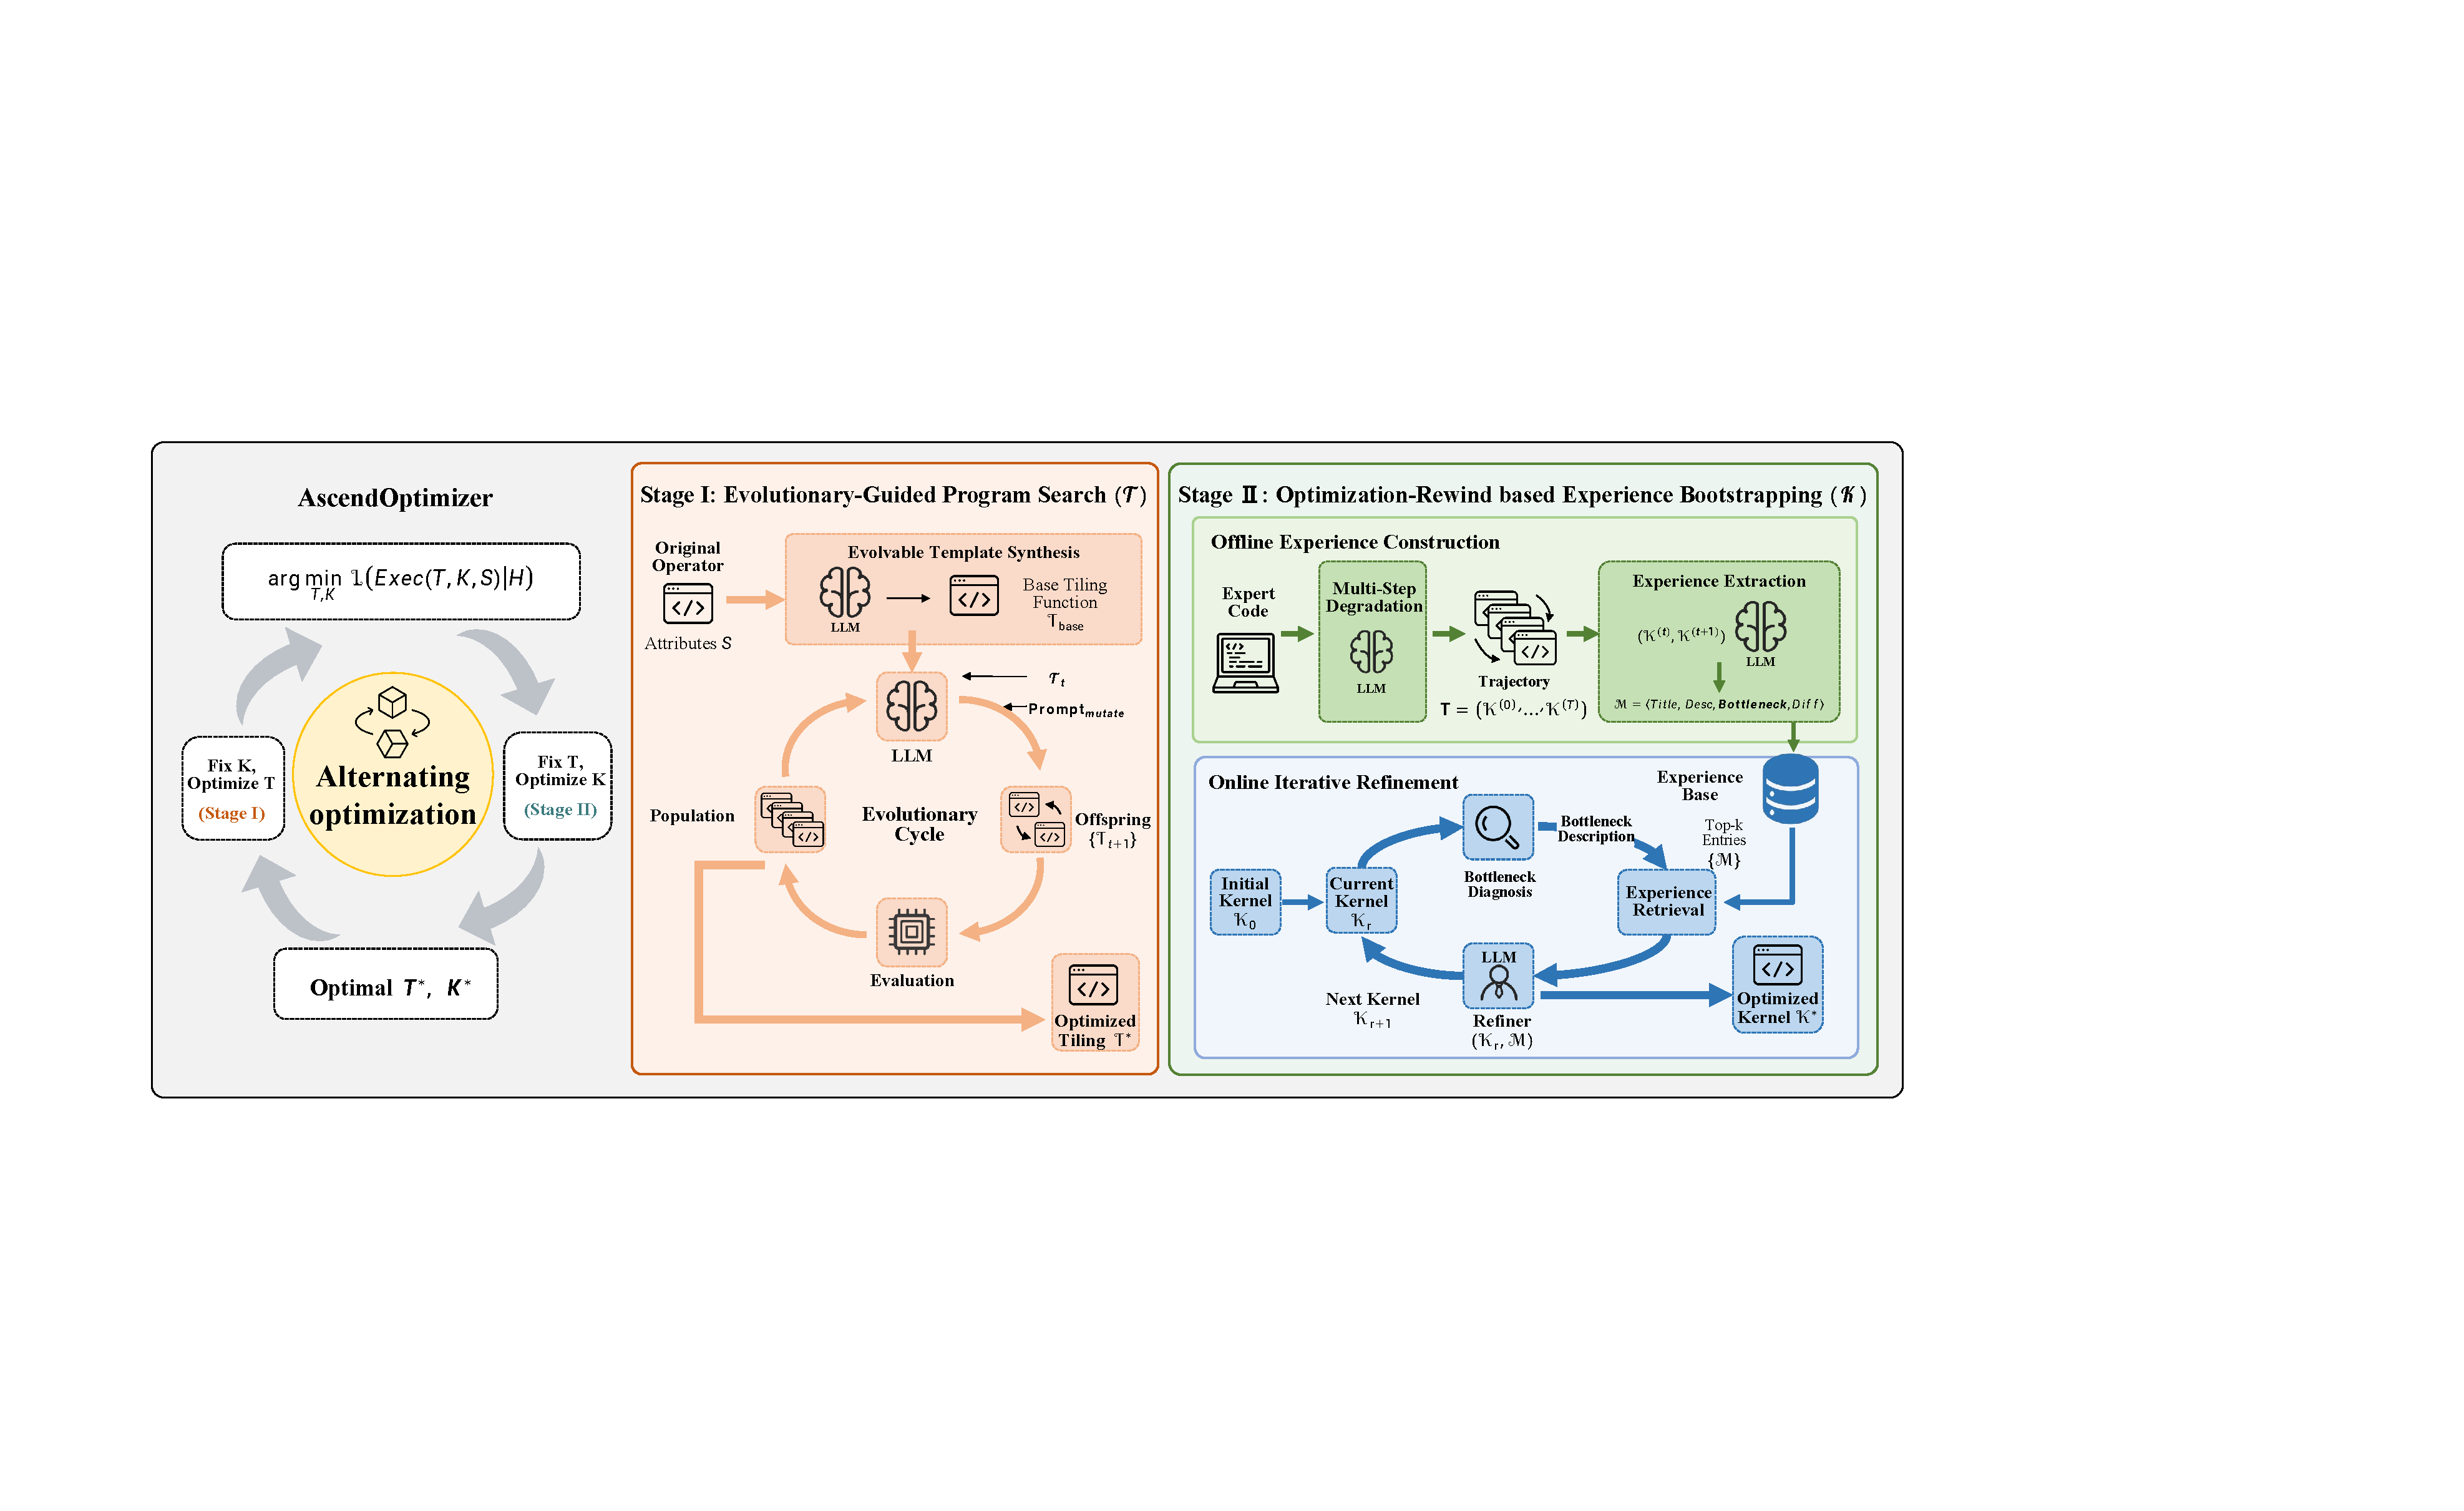
\includegraphics[width=\textwidth]{fig/framework-4.pdf}}
    \caption{Overview of \textbf{AscendOptimizer}. Stage \Rmnum{1} performs evolutionary-guided program search with hardware-in-the-loop profiling feedback to discover valid high-performance configurations; Stage \Rmnum{2} bootstraps optimization experience via optimization rewind and applies retrieval-augmented kernel optimization to address structural bottlenecks. The two stages are executed in an \emph{alternating loop}, where improvements from one stage feed into the other for progressive end-to-end optimization.}
    \label{framework}
  \end{center}
\end{figure*}

We first formalize the optimization of Ascend C operators as a dual search problem under heterogeneous computational constraints. Subsequently, we introduce the \textbf{AscendOptimizer} agent framework
% \footnote{Code and Dataset are available at \url{https://anonymous.4open.science/r/AscendOptimizer-3022/}.}
. Addressing the challenge of scarce expert experience in operator optimization, we design two complementary solving mechanisms tailored to the search space characteristics of the optimization targets: (1) for Tiling parameters, which exhibit strong implicit constraints and a highly discontinuous, fragmented solution landscape, we employ \textbf{Evolutionary-Guided Program Search}; (2) for Kernel code, which possesses high logical degrees of freedom and transferable optimization patterns, we utilize \textbf{Optimization-Rewind based Experience Bootstrapping}.

\subsection{Problem Setup}

In the Ascend NPU heterogeneous computing architecture, we formalize the operator task to be optimized as a tuple $\mathcal{O} = \langle \mathcal{T}, \mathcal{K}, \mathcal{S} \rangle$, where:
\begin{itemize}[leftmargin=*]
    \item $\mathcal{T} \in \mathbb{C}_{tiling}$: The tiling function running on the host side. It calculates data block sizes and movement instructions, directly determining the utilization of the on-chip UB and the saturation of the data movement pipeline.
    \item $\mathcal{K} \in \mathbb{C}_{kernel}$: The Kernel Code running on the AI Core. It governs instruction-level parallelism (ILP), vector unit utilization, and synchronization overhead.
    \item $\mathcal{S}$: The set of static operator attributes (e.g., Input Shape, Data Type, Layout).
\end{itemize}

Given a set of hardware constraints $H$ (e.g., buffer capacity, pipeline stages), our objective is to identify the optimal Tiling function $\mathcal{T}^*$ and Kernel implementation $\mathcal{K}^*$ that minimize the end-to-end execution latency on real hardware:
\begin{equation}
    (\mathcal{T}^*, \mathcal{K}^*) = \mathop{\arg\min}_{\mathcal{T}, \mathcal{K}} \mathcal{L}\left(\text{Exec}(\mathcal{T}, \mathcal{K}, \mathcal{S}) \mid H\right).
\end{equation}
Here, $\text{Exec}(\cdot)$ denotes hardware compilation and execution, and $\mathcal{L}$ denotes the measured latency. For brevity, when $H$ and $\mathcal{S}$ are fixed, we write $\mathcal{L}(\mathcal{K}\mid\mathcal{T}_{\text{curr}})$ as shorthand for $\mathcal{L}\!\left(\text{Exec}(\mathcal{T}_{\text{curr}}, \mathcal{K}, \mathcal{S}) \mid H\right)$ and omit $\text{Exec}(\cdot)$ and $H$. In Stage~\Rmnum{2}, $\mathcal{T}_{\text{curr}}$ is fixed only within one inner refinement loop; across outer alternating rounds, Stage~\Rmnum{1} can update $\mathcal{T}_{\text{curr}}$. Since $H$ contains numerous non-differentiable black-box constraints (e.g., bank conflicts, cache thrashing), and the code space $\mathbb{C}_{tiling} \times \mathbb{C}_{kernel}$ is highly discrete and non-convex, this problem is intractable via direct gradient descent.

\subsection{Overview}

AscendOptimizer optimizes the host-side tiling function $\mathcal{T}$ and the device-side kernel code $\mathcal{K}$ in two stages. While both problems lack reliable expert guidance, their search spaces have very different structures; accordingly, we adopt two complementary strategies:
\paragraph{Stage \Rmnum{1}: Evolutionary-Guided Program Search.} Tiling decisions are highly sensitive to Shape and Layout, exhibiting a discontinuous and fragmented landscape that is difficult to abstract into a general rule library. Consequently, we model Tiling optimization as a program search problem, leveraging LLMs to perform evolutionary search within the function space, implicitly learning hardware constraints via Hardware-in-the-Loop (HIL) feedback.
\paragraph{Stage \Rmnum{2}: Optimization-Rewind based Experience Bootstrapping.} Unlike Tiling, Kernel computation pipelines (e.g., Double Buffering, Vectorization) possess strong structural characteristics and transferability, yet the forward search space is vast. We construct a structured optimization pattern library via "Optimization Rewind" (deliberate de-optimization), transforming infinite code search into finite expert experience retrieval and application; in online optimization, each candidate kernel is still compiled and executed on real NPUs to obtain measured feedback for selection.

\subsection{Stage \Rmnum{1}: Evolutionary-Guided Program Search}

We elevate Tiling optimization to a constrained Program Search process. Distinct from the explicit experience retrieval in Stage \Rmnum{2}, this stage adopts an implicit exploration strategy. Since general Tiling rules cannot be predefined, we utilize hardware execution feedback as a ``boundary detector''. A zero-tolerance mechanism eliminates infeasible solutions, forcing the evolutionary algorithm to converge automatically to optimal configurations within the implicit feasible region of the hardware.

Traditional compiler autotuning usually assumes a relatively smooth parameter landscape. In contrast, our LLM-driven mutation leverages semantic priors to guide code-level exploration and bias candidates toward hardware-feasible regions. Unlike template-bound numerical tuning, it also supports lightweight structural rewrites (e.g., dynamic boundary handling), helping the search escape discontinuous regions where conventional methods often stagnate.

\begin{itemize}
\item \textbf{Evolvable Template Synthesis.}
First, the LLM analyzes the original operator code and attributes $\mathcal{S}$ to identify key logic blocks controlling data partitioning and movement. The system automatically synthesizes a base tiling function $\mathcal{T}_{base}$ containing ``evolution markers'' (see Appendix~\ref{app:methodDet}, Fig.~\ref{fig:appendix_tiling_code}). This process goes beyond parameter extraction by functionalizing loop structures and conditional branches, thereby defining the initial search space for evolution.

\item \textbf{LLM-based Function Mutation.}
We treat each Tiling function as an individual $I = \mathcal{T}$ and employ the LLM as an intelligent mutation operator $\mathcal{M}_{LLM}$. In generation $t$, the LLM generates offspring based on the code structure of the parent individual and historical performance feedback:
\begin{equation}
    \mathcal{T}_{t+1} \sim \mathcal{M}_{LLM}(\mathcal{T}_t, \text{Prompt}_{\text{mutate}}).
\end{equation}
Mutation operations cover two dimensions: 
(1) Parameter Fine-tuning, such as adjusting ``BlockDim''; and 
(2) Logic Rewriting, such as altering the computation logic of ``TilingKey'' or memory alignment strategies. 
This mechanism allows to break through fixed template limitations and explore structural optimization opportunities.

\item \textbf{Rigorous Hardware-in-the-Loop Evaluation.}
To address the difficulty of explicitly formalizing Tiling experience, we directly use NPU execution feedback as the fitness function. We adopt a zero-tolerance strategy to filter invalid individuals:
\begin{equation}
\label{eq:fitness}
f(\mathcal{T})=
\begin{cases}
\dfrac{1}{\mathcal{L}\!\left(\mathrm{Exec}\!\left(\mathcal{T},\mathcal{K}_{\text{base}},\mathcal{S}\right) \mid H\right)},
& \text{Success},\\[15pt] % 增加行间距，防止拥挤
\text{Discard},
& \begin{aligned}
& \text{CompileFail or PrecisionError}.
\end{aligned}
\end{cases}
\end{equation}
Any $\mathcal{T}$ resulting in compilation failure or precision anomalies is immediately removed from the population. This strong constraint mechanism ensures the evolutionary process rapidly filters out invalid search paths, focusing on high-performance regions that satisfy implicit hardware constraints (e.g., address alignment, buffer limits).
\end{itemize}


\subsection{Stage \Rmnum{2}: Optimization-Rewind based Experience Bootstrapping}

% While degradation concepts are theoretically applicable to all code components, Kernel logic (e.g., pipeline masking, instruction scheduling) is more structured and dependent on expert patterns than Tiling parameters. Therefore, we implement Optimization-Rewind based Experience Bootstrapping specifically for the Kernel.

% \noindent\textbf{Self-Supervised Experience Construction.}
% To learn the path from inefficient to efficient implementations, we execute a multi-step degradation process on an expert dataset $\mathcal{C}_{expert}$ to construct the inverse optimization process.

% \textit{Multi-Step Dynamic Degradation.} Leveraging the code understanding capabilities of LLMs, we perform continuous multi-step degradation on expert code $\mathcal{K}_{expert}$ to form a trajectory $\mathbb{T} = (\mathcal{K}^{(0)}, \mathcal{K}^{(1)}, \dots, \mathcal{K}^{(T)})$, where $\mathcal{K}^{(0)} = \mathcal{K}_{expert}$. In step $t$, the LLM analyzes $\mathcal{K}^{(t)}$ and injects performance defects to generate $\mathcal{K}^{(t+1)}$:
% \begin{equation}
%     \mathcal{K}^{(t+1)} = \text{LLM}_{\text{rewind}}(\mathcal{K}^{(t)}, \mathbb{P}_{deg}).
% \end{equation}
% Here, $\mathbb{P}_{deg}$ represents the degradation operator space (e.g., "breaking pipeline masking", "removing vectorized loops"). This simulates the gradual deterioration of code performance as optimization techniques are removed.
% After each degradation step, we benchmark the resulting variant on real hardware. Since such measurements can be noisy, we introduce a preset tolerance threshold $\delta$(chosen empirically) and treat a removal as effective only when the observed performance drop exceeds $\delta$.

% \textit{Differential Threshold Filtering and Tuple Extraction.} Not all degradation steps possess learning value. We select only adjacent node pairs $(\mathcal{K}^{(t+1)}, \mathcal{K}^{(t)})$ with significant performance differences for experience extraction, satisfying $\mathcal{L}(\mathcal{K}^{(t+1)}) - \mathcal{L}(\mathcal{K}^{(t)}) > \delta$. For selected pairs, the LLM compares and extracts a structured optimization experience quadruple $\mathcal{M}$:
% \begin{equation}
%     \mathcal{M} = \langle \text{Title}, \text{Desc}, \text{Bottleneck}, \text{Diff} \rangle,
% \end{equation}
% where $\text{Bottleneck}$ describes the specific performance bottleneck in $\mathcal{K}^{(t+1)}$ (e.g., "Scalar instructions blocking vector pipe"), serving as the index key for subsequent retrieval.

% \noindent\textbf{Iterative Retrieval and Refinement.}
% During inference, we adopt a multi-round optimization loop to progressively improve the target kernel $\mathcal{K}_{\text{target}}$. We initialize $\mathcal{K}_0 = \mathcal{K}_{\text{target}}$ and, at each round $r$, perform three steps: (i) \emph{bottleneck diagnosis}, where a diagnostic model compares static code features of good vs.\ bad kernels together with their measured hardware runtime feedback to infer the bottleneck and form a query $q_{\text{bottleneck}}^{(r)}$; (ii) \emph{experience retrieval}, where we compute similarity between $q_{\text{bottleneck}}^{(r)}$ and the indexed keys $v_{\text{key}}$ to retrieve the Top-$k$ most relevant optimization tuples $\{\mathcal{M}_i\}_{i=1}^k$ from the experience bank; and (iii) \emph{context-aware refinement}, where the Refiner LLM rewrites $\mathcal{K}_r$ guided by the retrieved patterns to obtain the next version, which is then compiled and executed on real NPUs to obtain the measured feedback for selection:
% \begin{equation}
%     \mathcal{K}_{r+1} = \text{Refiner}(\mathcal{K}_r, \{\mathcal{M}_i\}_{i=1}^k).
% \end{equation}

% We repeat this loop until reaching a preset number of rounds or observing performance convergence. The round-wise structure encourages hierarchical debugging and optimization (e.g., fixing memory access conflicts before tuning instruction scheduling), enabling deeper improvements than single-shot rewriting.



While Stage \Rmnum{1} identifies the optimal parameters for a fixed code structure, it cannot overcome fundamental architectural bottlenecks (e.g., pipeline stalls or missing double-buffering). To address the chronic scarcity of expert-level data in the Ascend ecosystem, we propose \textbf{Optimization-Rewind}, a self-supervised mechanism that transforms a small set of high-performance seed kernels into a retrievable experience bank.

\subsubsection{Inverse Experience Distillation via Rewind}
Instead of searching for optimizations in a vacuum, we perform a systematic \textit{reverse-engineering} on a seed set of expert-level kernels $\mathcal{K}_{expert}$. 

\begin{enumerate}[leftmargin=*]
    \item \textbf{Stepwise De-optimization (Rewind):} Starting from $\mathcal{K}_{expert}$, an LLM acts as an ``inverse agent'' that identifies and systematically removes specific optimization motifs---such as unrolling loops, breaking pipeline masking, or reverting vectorized intrinsics to scalar implementations. This generates a trajectory of decreasing performance: $\mathbb{T} = (\mathcal{K}^{(0)}, \mathcal{K}^{(1)}, \dots, \mathcal{K}^{(T)})$, where $\mathcal{K}^{(0)} = \mathcal{K}_{expert}$.
    \item \textbf{Hardware-Grounded Validation:} Each variant is executed on the NPU. We only retain pairs $(\mathcal{K}^{(t+1)}, \mathcal{K}^{(t)})$ where the observed latency $\mathcal{L}(\mathcal{K}^{(t+1)})$ significantly exceeds $\mathcal{L}(\mathcal{K}^{(t)})$. This ensures that each rewound feature is a verified performance driver under real hardware constraints.
    \item \textbf{Semantic Distillation:} For each validated pair, the LLM analyzes the code diff alongside hardware profiling signals to distill a structured \textbf{Optimization Tuple} $\mathcal{M}$:
    \begin{equation}
        \mathcal{M} = \langle \text{Title, Description, Bottleneck, Code Diff} \rangle.
    \end{equation}
    Here, \textit{Bottleneck} is used as the primary retrieval key (via embedding), while \textit{Description} and \textit{Code Diff} provide the actionable context for rewriting. This converts raw code deltas into semantic expertise (e.g., identifying that a specific synchronization removal caused an MTE2 pipeline stall), forming a retrievable \textbf{Experience Bank}.
\end{enumerate}

\subsubsection{Retrieval-Augmented Kernel Refinement}
During the online optimization of a target operator, the agent treats refinement as an episodic retrieval-and-apply task:

\begin{itemize}[leftmargin=*]
    \item \textbf{Bottleneck Diagnosis:} The agent analyzes the target kernel $\mathcal{K}_{curr}$ and its profiling traces to formulate a diagnostic query $q$.
    \item \textbf{Experience Retrieval:} A dense retriever fetches the Top-$k$ tuples $\{\mathcal{M}_i\}_{i=1}^k$ from the Experience Bank whose symptoms best match the current bottleneck.
    \item \textbf{Knowledge-Guided Rewriting:} A Refiner LLM applies the retrieved expert patterns to rewrite $\mathcal{K}_{curr}$. Each rewritten candidate is then compiled and evaluated on real hardware; only variants that pass compilation and improve measured latency are retained for the next iteration.
\end{itemize}

\subsection{Alternating Optimization of Tiling and Kernel}

Tiling and kernel optimizations often target different hardware constraints (e.g., data layout and on-chip resource limits), so applying them simultaneously can create conflicting behaviors. To prevent local gains from introducing new bottlenecks, we adopt an alternating strategy with explicit time scales: in each Stage~\Rmnum{2} inner loop, $\mathcal{T}$ is fixed while $\mathcal{K}$ is refined; after that inner loop, Stage~\Rmnum{1} resumes and may update $\mathcal{T}$ for the next outer round. This iterative handoff keeps updates feasible and makes the two optimizers synergistic within the execution environment (see Algorithm~\ref{alg:alternating_optimization}).

\begin{algorithm}[!t]
\small
\setlength{\abovecaptionskip}{2pt}
\setlength{\belowcaptionskip}{2pt}
\caption{AscendOptimizer}
\label{alg:alternating_optimization}
\begin{algorithmic}[1]
\Require Initial tiling program $\mathcal{T}^{(0)}$, initial kernel $\mathcal{K}^{(0)}$;
\Require Evaluation function $\mathcal{L}(\cdot)$, outer rounds $R$, Stage~\Rmnum{1} steps $U$, Stage~\Rmnum{2} steps $S$;
\Output Best pair $(\mathcal{T}^{\dagger}, \mathcal{K}^{\dagger})$;
\State $(\mathcal{T}^{\dagger}, \mathcal{K}^{\dagger}) \gets (\mathcal{T}^{(0)}, \mathcal{K}^{(0)})$;
\State $\ell^{\dagger} \gets \mathcal{L}(\mathcal{T}^{\dagger}, \mathcal{K}^{\dagger})$;
\For{$r = 1$ to $R$}
    \State \textbf{Inherit current best:} $(\mathcal{T}^{(r,0)}, \mathcal{K}^{(r,0)}) \gets (\mathcal{T}^{\dagger}, \mathcal{K}^{\dagger})$

    \State \textbf{(Stage \Rmnum{1})} Optimize $\mathcal{T}$ with $\mathcal{K}^{\dagger}$ fixed:
    \State $\mathcal{T}_{\text{best}}^{(r)} \gets \mathcal{T}^{(r,0)}$, $\ell_{T,\text{best}}^{(r)} \gets \mathcal{L}(\mathcal{T}_{\text{best}}^{(r)}, \mathcal{K}^{\dagger})$
    \For{$u = 1$ to $U$}
        \State $\tilde{\mathcal{T}} \gets \textsc{TilingSearchStep}(\mathcal{T}_{\text{best}}^{(r)}, \mathcal{K}^{\dagger})$;
        \If{$\tilde{\mathcal{T}}$ compiles and passes correctness}
            \State $\tilde{\ell}_T \gets \mathcal{L}(\tilde{\mathcal{T}}, \mathcal{K}^{\dagger})$;
            \If{$\tilde{\ell}_T < \ell_{T,\text{best}}^{(r)}$}
                \State $\mathcal{T}_{\text{best}}^{(r)} \gets \tilde{\mathcal{T}}$, $\ell_{T,\text{best}}^{(r)} \gets \tilde{\ell}_T$;
            \EndIf
        \EndIf
    \EndFor

    \State \textbf{(Stage \Rmnum{2})} Optimize $\mathcal{K}$ with inherited $\mathcal{T}_{\text{best}}^{(r)}$ fixed:
    \State $\mathcal{K}_{\text{best}}^{(r)} \gets \mathcal{K}^{\dagger}$, $\ell_{K,\text{best}}^{(r)} \gets \mathcal{L}(\mathcal{T}_{\text{best}}^{(r)}, \mathcal{K}_{\text{best}}^{(r)})$;
    \For{$s = 1$ to $S$}
        \State $\tilde{\mathcal{K}} \gets \textsc{KernelRefine}(\mathcal{T}_{\text{best}}^{(r)}, \mathcal{K}_{\text{best}}^{(r)})$;
        \If{$\tilde{\mathcal{K}}$ compiles and passes correctness}
            \State $\tilde{\ell}_K \gets \mathcal{L}(\mathcal{T}_{\text{best}}^{(r)}, \tilde{\mathcal{K}})$;
            \If{$\tilde{\ell}_K < \ell_{K,\text{best}}^{(r)}$}
                \State $\mathcal{K}_{\text{best}}^{(r)} \gets \tilde{\mathcal{K}}$, $\ell_{K,\text{best}}^{(r)} \gets \tilde{\ell}_K$;
            \EndIf
        \EndIf
    \EndFor

    \State \textbf{Round inheritance:} $(\mathcal{T}^{\dagger}, \mathcal{K}^{\dagger}) \gets (\mathcal{T}_{\text{best}}^{(r)}, \mathcal{K}_{\text{best}}^{(r)})$;
    \State $\ell^{\dagger} \gets \ell_{K,\text{best}}^{(r)}$;
\EndFor
\State \Return $(\mathcal{T}^{\dagger}, \mathcal{K}^{\dagger})$.
\end{algorithmic}
%\vspace{-0.5em}
\end{algorithm}





\section{Experiments}
\label{sec:experiments}

% We build our benchmark from Huawei's open-source AscendC operator repository \texttt{cann-ops}\footnote{\url{https://gitee.com/ascend/cann-ops}}, using its implementations as performance baselines. We (i) validate compilability and numerical correctness, (ii) adjust input shapes for a subset of operators to reduce measurement noise, and (iii) filter out invalid cases; this yields a final set of 133 operators for evaluation.

We construct our benchmark using the Huawei official AscendC repository, \texttt{cann-ops}\footnote{\url{https://gitee.com/ascend/cann-ops}}, adopting its implementations as performance baselines. The preparation process involves verifying compilability and numerical correctness against a CPU reference, followed by removing operators that fail to execute or meet accuracy standards. This filtering process results in a final evaluation set of 127 operators.

\subsection{Hardware and Metrics}
\label{sec:hardware_metrics}


\paragraph{Hardware and Software Stack.}

Experiments are performed on Huawei Ascend 910B4 NPUs using the CANN 8.3 software stack. To ensure reproducibility, we maintain a unified configuration across all operators, including identical toolchains, stream settings, and synchronization mechanisms.

\paragraph{Correctness.}

Numerical accuracy is verified by comparing NPU outputs with CPU references through an elementwise tolerance check. We apply both absolute and relative tolerances, which are adjusted based on the specific operator and data type. An operator is marked as correct if the proportion of elements exceeding these thresholds remains below a predefined limit. This protocol follows the standard tolerance policies provided in official CANN examples.



\paragraph{Performance.}
We report latency and relative speedup over the \texttt{cann-ops} baseline:
\begin{equation}
\mathrm{speedup}(op) = \frac{T_{\mathrm{baseline}}(op)}{T_{\mathrm{gen}}(op)}.
\end{equation}
Each operator is warmed up before measurement and timed for multiple repetitions.
We additionally report $\mathrm{fast}_p$, the fraction of operators with speedup greater than $p$:
\begin{equation}
\mathrm{fast}_p = \frac{\left|\left\{ op \mid \mathrm{speedup}(op) > p \right\}\right|}{\left|\mathcal{O}\right|}.
\end{equation}

% \noindent\textbf{Input Shapes and Operator Filtering.}
% To reduce measurement noise, we moderately increase input sizes for some operators while preserving semantics.
% We filter out operators that fail to compile/run or violate correctness, and retain 133 operators for evaluation.
\paragraph{Benchmark construction and filtering.}
We start from the \texttt{cann-ops} AscendC operator repository and use the provided implementations as our baseline.
During preparation, we (i) verify compilability, (ii) check numerical correctness against a CPU reference, and (iii) remove operators that fail compilation/execution or violate correctness.

\paragraph{Input-shape adjustment (noise reduction).}
Because hardware-level timing can be noisy for small workloads, we moderately increase the input shapes for a subset of operators to improve runtime stability and make performance differences more observable. To minimize threats to validity, we follow three safeguards: (i) we only apply shape changes that preserve operator semantics (e.g., scaling batch/sequence/spatial dimensions without changing the computation type); (ii) for each affected operator, we evaluate \emph{both} the baseline and all optimized variants under the \emph{same} adjusted shape (so reported speedups remain comparable); and (iii) we keep the scaling factor small and report the original and adjusted shapes in this appendix.
 
\paragraph{Clarification on Evaluation Paradigm and Data Overlap.}
It is important to note that the seed kernels used to construct the offline experience bank in Stage II are derived from the same set of 127 benchmark operators. Unlike standard predictive machine learning tasks where overlapping train and test sets cause data leakage and undermine zero-shot generalization, AscendOptimizer follows the classical system auto-tuning paradigm. Our framework operates as a training-free episodic agent that uses Retrieval-Augmented Generation (RAG); no model weights are updated. The objective is transductive: to discover the absolute lowest latency for a given target workload on specific hardware. Therefore, "overfitting" the optimization strategies to the target operators and the Ascend architecture is the explicit goal of the system, rather than a methodological flaw.
% \begin{table*}[h]
% \centering
% \small
% \renewcommand{\arraystretch}{1.2}
% % \resizebox{\linewidth}{!}{%
% \begin{tabularx}{\columnwidth}{|l|c|c|c|c|c|}
% \hline
% Method & GM & Fast$_{1.0}$ & Fast$_{1.2}$ & Fast$_{1.4}$ & Fast$_{2.0}$ \\
% \hline
% \multicolumn{6}{|l|}{\textbf{Best-of-N baselines}} \\
% \hline
% BoN@5 (DeepSeek-Chat) & 1.17 & 4.51\% & 3.01\% & 1.50\% & 1.50\% \\
% BoN@40 (DeepSeek-Chat) & 1.20 & 18.05\% & 6.77\% & 4.51\% & 1.5\% \\
% \hline

% \multicolumn{6}{|l|}{\textbf{Agent / Search baselines}} \\
% \hline
% OpenEvolve & -- & -- & -- & -- & -- \\
% \hline

% \multicolumn{6}{|l|}{\textbf{Ours}} \\
% \hline
% EvoAscend & 1.50 & 46.62\% & 16.54\% & 12.78\% & 9.02\% \\
% \hline

% \end{tabularx}%
% % }
% \caption{Main Performance.BoN@N: sample N complete kernels and pick the fastest based on measured duration.GM denotes geometric mean speedup over the reference implementation.}
% \label{tab:main_performance}
% \end{table*}

% Suggested packages:
% \usepackage{booktabs}
% \usepackage{tabularx}

% Suggested packages:
% \usepackage{booktabs}

% Suggested packages:
% \usepackage{booktabs}
% \usepackage{tabularx}

% Suggested packages:
% \usepackage{booktabs}
% \usepackage{tabularx}
\subsection{Main Results}

We adopt a heterogeneous model deployment strategy to balance high-level code reasoning with iterative inference efficiency. For structural initialization and offline tasks—specifically, Evolvable Template Synthesis in Stage \Rmnum{1} and Self-Supervised Experience Construction in Stage \Rmnum{2}—we utilize GPT-5.2. Conversely, for the dynamic online optimization loops, we employ DeepSeek-V3.2 to drive both the LLM-based Function Mutation in Stage \Rmnum{1} and the Iterative Retrieval and Refinement in Stage \Rmnum{2}. Consequently, the Stage \Rmnum{2} evaluation relies on an experience bank built during the offline rewind phase by GPT-5.2, which contains 412 distinct optimization tuples.

% \begin{figure}[!t]
%   \centering
%   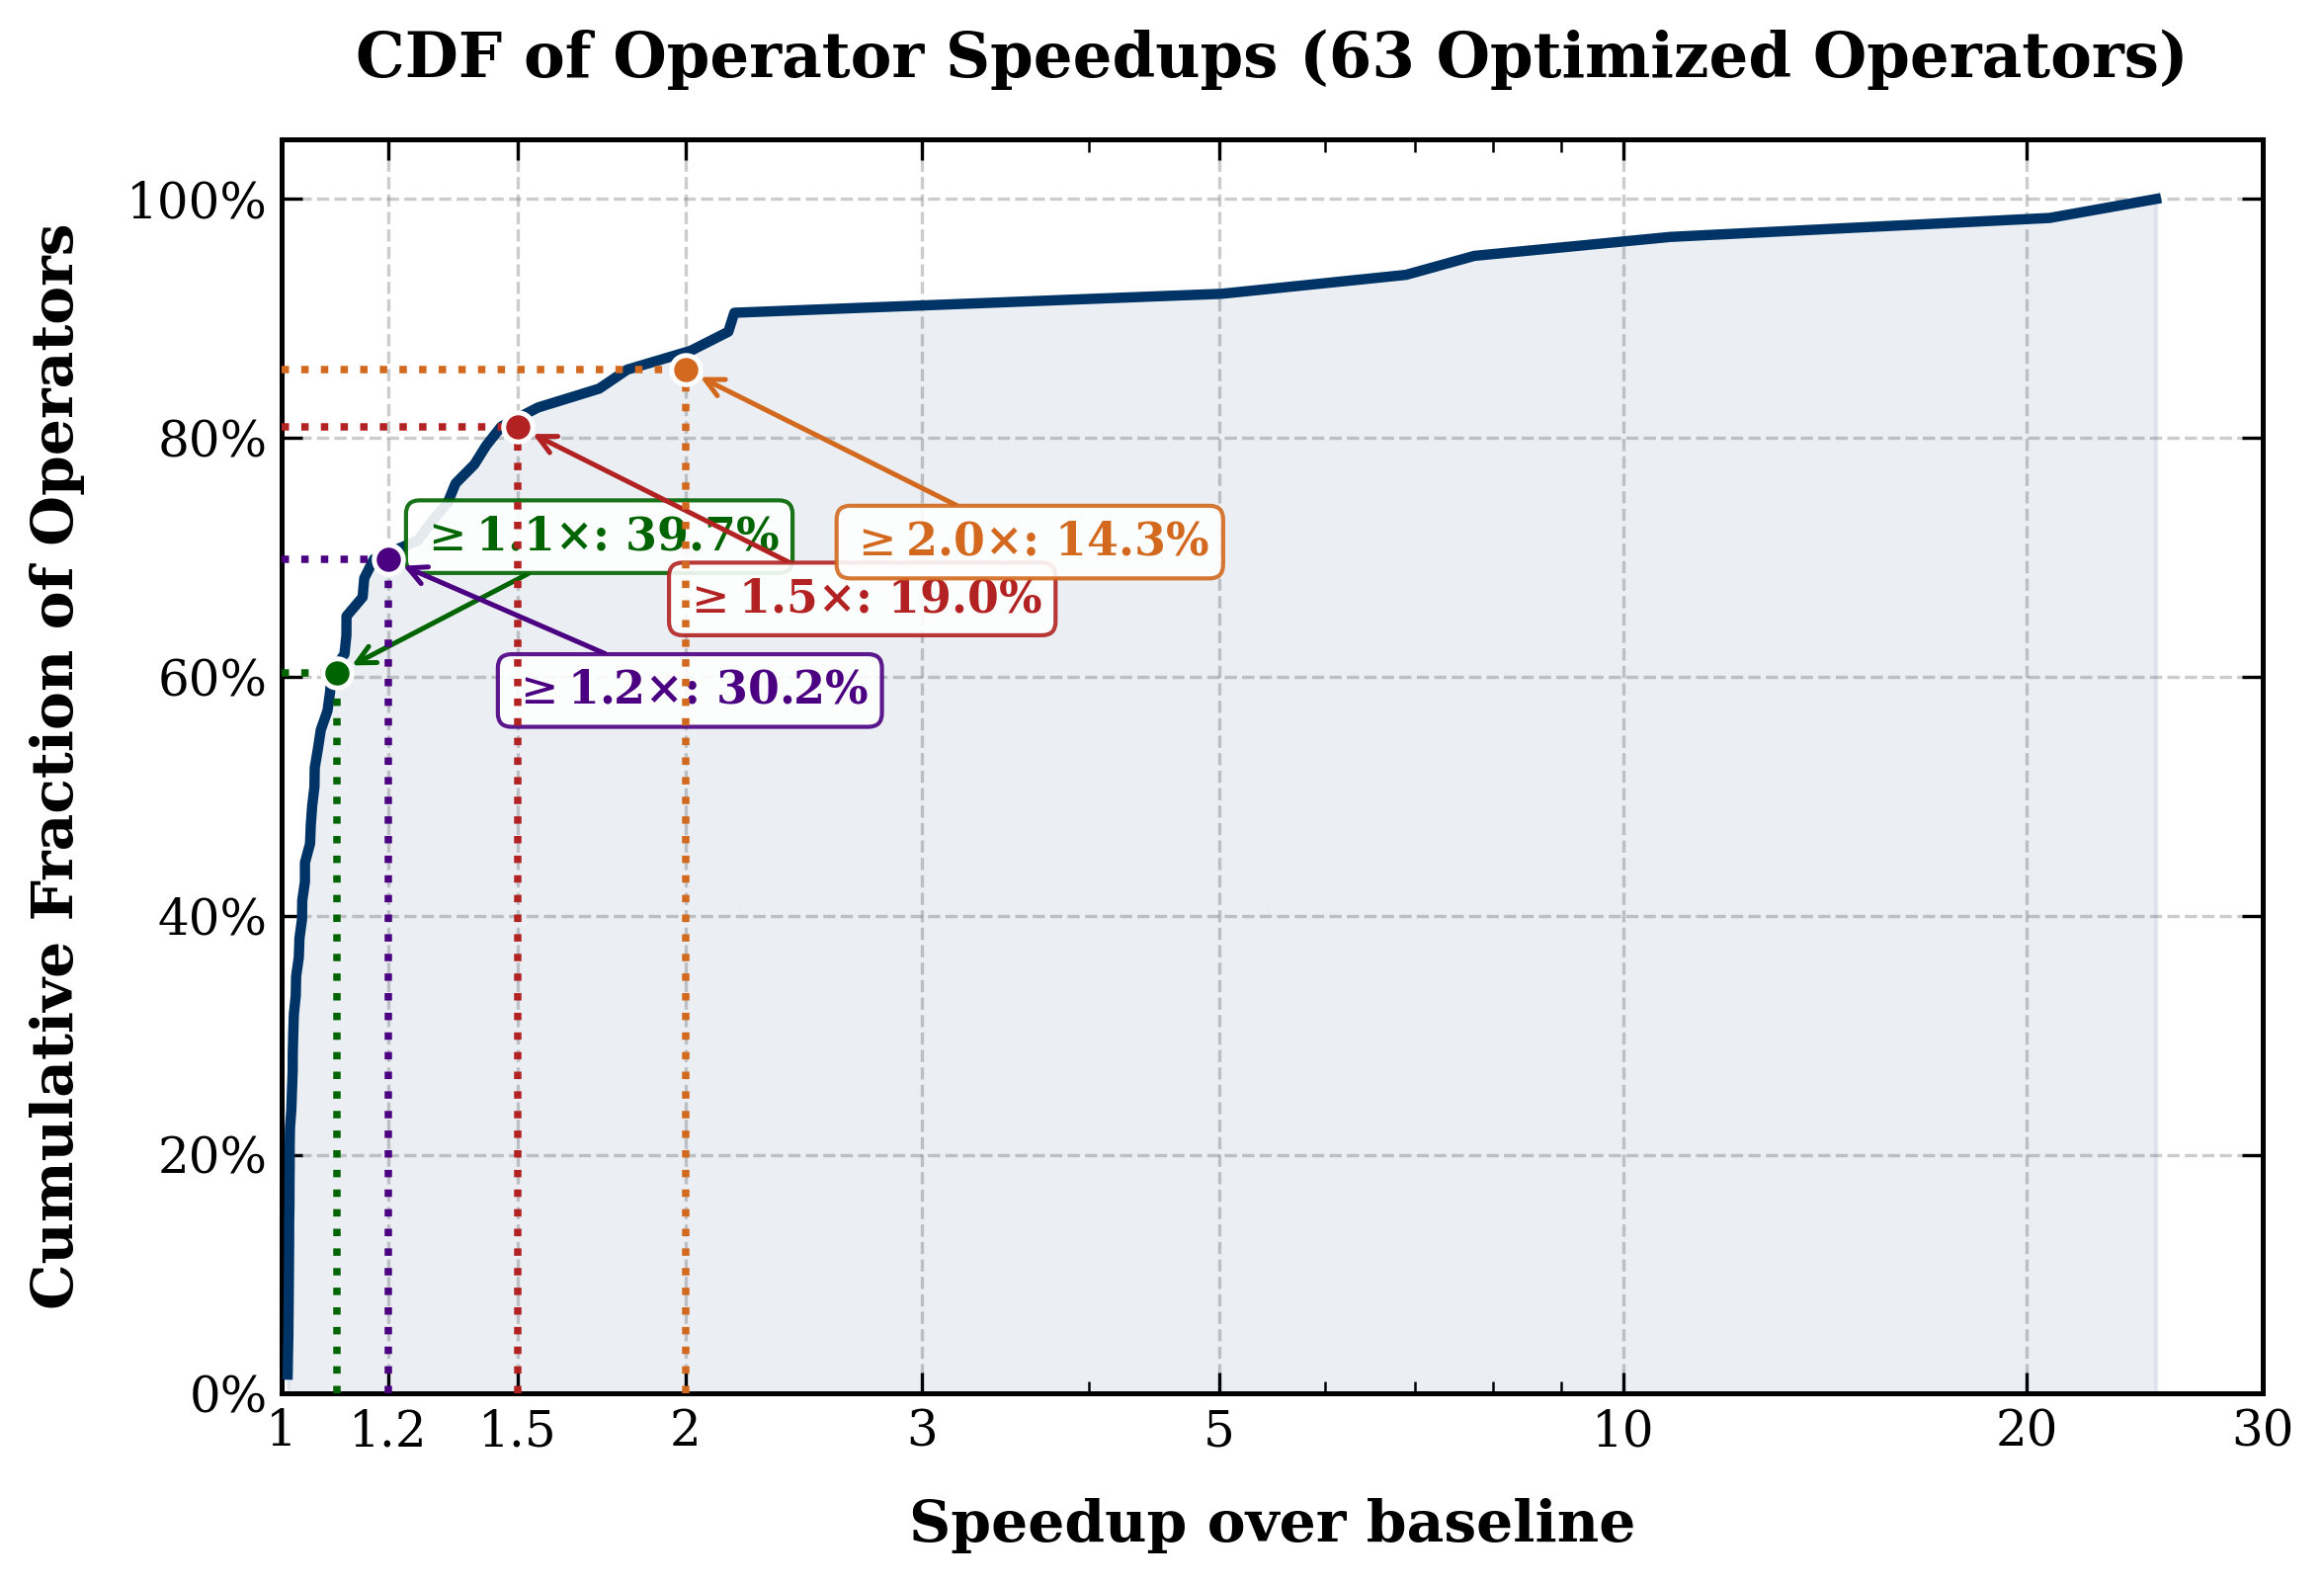
\includegraphics[width=0.64\linewidth]{fig/speedup_distribution.png}
%   \caption{CDF of per-operator speedups achieved by \textbf{AscendOptimizer} on 63 optimized operators. The x-axis is the speedup over the baseline and the y-axis is the cumulative fraction of operators. Dashed markers highlight the corresponding tail ratios: \SI{39.7}{\percent} of operators achieve at least $1.1\times$, \SI{30.2}{\percent} achieve at least $1.2\times$, \SI{19.0}{\percent} achieve at least $1.5\times$, and \SI{14.3}{\percent} achieve at least $2.0\times$.}
%   \label{fig:improvement}
% \end{figure}


Table~\ref{tab:main_performance} reports level-wise results with explicit sample counts (level1/level2/level3 contain 43/77/7 operators, respectively). For each level, we report the geometric-mean speedup (GM) and the $\text{fast}_x$ ratios for $x \in \{1.0, 1.2, 1.4, 2.0\}$, where higher is better.
Across all three levels, increasing pure sampling from BoN@5 to BoN@40 yields only modest gains. OpenEvolve~\cite{openevolve} generally outperforms BoN, supporting the benefit of iterative refinement over one-shot sampling.
\textbf{AscendOptimizer} achieves the best overall results, with GM values of 1.08/1.21/1.81 on level1/level2/level3 and fast$_{1.0}$ ratios of \SI{46.51}{\percent}/\SI{49.35}{\percent}/\SI{71.43}{\percent}. On level3, fast$_{1.2}$, fast$_{1.4}$, and fast$_{2.0}$ reach \SI{28.57}{\percent}; compared with OpenEvolve, this corresponds to ties on fast$_{1.2}$ and fast$_{1.4}$ and a clear lead on fast$_{2.0}$.

% \begin{table}[t]
% \centering
% \caption{\textbf{Main performance.} \textbf{GM} denotes the geometric-mean speedup relative to the reference implementation (higher is better). \textbf{$fast_p$} denotes the fraction of test cases that achieve at least an $x\times$ speedup. BoN@$N$ samples $N$ complete kernels and selects the fastest candidate according to measured runtime. For the BoN and OpenEvolve baselines, we expose the complete operator implementation (host and kernel code) to the optimizer.All methods are given the same compilation/profiling interface and the same optimization budget (40 iterations and DeepSeek-V3.2)}
% \label{tab:main_performance}
% \setlength{\tabcolsep}{3pt}
% \small
% \begin{tabularx}{\columnwidth}{@{}l l *{5}{>{\centering\arraybackslash}X}@{}}
% \toprule
% \textbf{Category} & \textbf{Method} & \textbf{GM} $\uparrow$ & \textbf{fast$_{1.0}$} $\uparrow$ & \textbf{fast$_{1.2}$} $\uparrow$ & \textbf{fast$_{1.4}$} $\uparrow$ & \textbf{fast$_{2.0}$} $\uparrow$ \\
% \midrule
% \textit{Best-of-$N$} & BoN@5  & \heatcell{1.02}{1.02}{1.21}{1.02} & \heatcell{4.51}{4.51}{46.62}{\SI{4.51}{\percent}} & \heatcell{3.01}{3.01}{15.79}{\SI{3.01}{\percent}} & \heatcell{1.50}{1.50}{12.03}{\SI{1.50}{\percent}} & \heatcell{1.50}{1.50}{8.27}{\SI{1.50}{\percent}} \\
% \textit{Best-of-$N$} & BoN@40 & \heatcell{1.05}{1.02}{1.21}{1.05} & \heatcell{18.05}{4.51}{46.62}{\SI{18.05}{\percent}} & \heatcell{6.77}{3.01}{15.79}{\SI{6.77}{\percent}} & \heatcell{4.51}{1.50}{12.03}{\SI{4.51}{\percent}} & \heatcell{1.50}{1.50}{8.27}{\SI{1.50}{\percent}} \\
% \midrule
% \textit{Agent/Search} & OpenEvolve & \heatcell{1.10}{1.02}{1.21}{1.10} & \heatcell{27.07}{4.51}{46.62}{\SI{27.07}{\percent}} & \heatcell{7.52}{3.01}{15.79}{\SI{7.52}{\percent}} & \heatcell{6.02}{1.50}{12.03}{\SI{6.02}{\percent}} & \heatcell{4.51}{1.50}{8.27}{\SI{4.51}{\percent}} \\
% \midrule
% \textit{Ours} & \textbf{AscendOptimizer} & \heatcell{1.34}{1.02}{1.34 }{\textbf{1.34}} & \heatcell{51.88}{4.51}{51.88}{\textbf{\SI{51.88}{\percent}}} & \heatcell{19.55}{3.01}{19.55}{\textbf{\SI{19.55}{\percent}}} & \heatcell{15.79}{1.50}{15.79}{\textbf{\SI{15.79}{\percent}}} & \heatcell{12.03}{1.50}{12.03}{\textbf{\SI{12.03}{\percent}}} \\
% \bottomrule
% \end{tabularx}
% \end{table}


\begin{table}[htbp]
\centering
\caption{\textbf{Main performance.} \textbf{GM} denotes the geometric-mean speedup relative to the reference implementation (higher is better). \textbf{$fast_p$} denotes the fraction of test cases that achieve at least an $x\times$ speedup. BoN@$N$ samples $N$ complete kernels and selects the fastest candidate according to measured runtime. For the BoN and OpenEvolve baselines, we expose the complete operator implementation (host and kernel code) to the optimizer. All methods are given the same compilation/profiling interface and the same optimization budget (40 iterations and DeepSeek-V3.2).}
\label{tab:main_performance}
\setlength{\tabcolsep}{3pt}
\small
\begin{tabularx}{\columnwidth}{@{}l c l *{5}{>{\centering\arraybackslash}X}@{}}
\toprule
\textbf{Level} & \textbf{Tasks} & \textbf{Method} & \textbf{GM} $\uparrow$ & \textbf{fast$_{1.0}$} $\uparrow$ & \textbf{fast$_{1.2}$} $\uparrow$ & \textbf{fast$_{1.4}$} $\uparrow$ & \textbf{fast$_{2.0}$} $\uparrow$ \\
\midrule

\multirow{4}{*}{level1}
& \multirow{4}{*}{43} & BoN@5 & \heatcell{1.01}{1.01}{1.22}{1.01} & \heatcell{9.09}{8.89}{48.89}{9.09\%} & \heatcell{2.27}{2.22}{13.33}{2.27\%} & \heatcell{0.00}{0.00}{13.33}{0.00\%} & \heatcell{0.00}{0.00}{8.89}{0.00\%} \\
& & BoN@40 & \heatcell{1.02}{1.01}{1.22}{1.02} & \heatcell{11.63}{8.89}{48.89}{11.63\%} & \heatcell{2.33}{2.22}{13.33}{2.33\%} & \heatcell{2.33}{0.00}{13.33}{2.33\%} & \heatcell{0.00}{0.00}{8.89}{0.00\%} \\
& & OpenEvolve & \heatcell{1.02}{1.01}{1.22}{1.02} & \heatcell{16.28}{8.89}{48.89}{16.28\%} & \heatcell{4.65}{2.22}{13.33}{4.65\%} & \heatcell{2.33}{0.00}{13.33}{2.33\%} & \heatcell{0.00}{0.00}{8.89}{0.00\%} \\
& & \textbf{AscendOptimizer} & \heatcell{1.08}{1.01}{1.08}{1.08} & \heatcell{45.45}{8.89}{45.45}{46.51\%} & \heatcell{6.82}{2.22}{6.82}{6.98\%} & \heatcell{6.82}{0.00}{6.82}{6.98\%} & \heatcell{2.27}{0.00}{2.27}{2.33\%} \\

\midrule

\multirow{4}{*}{level2}
& \multirow{4}{*}{77} & BoN@5 & \heatcell{1.02}{1.02}{1.29}{1.02} & \heatcell{12.99}{12.66}{50.63}{12.99\%} & \heatcell{2.60}{2.53}{20.25}{2.60\%} & \heatcell{2.60}{2.53}{13.92}{2.60\%} & \heatcell{2.60}{2.53}{10.13}{2.60\%} \\
& & BoN@40 & \heatcell{1.04}{1.02}{1.29}{1.04} & \heatcell{19.48}{12.66}{50.63}{19.48\%} & \heatcell{6.49}{2.53}{20.25}{6.49\%} & \heatcell{3.90}{2.53}{13.92}{3.90\%} & \heatcell{1.30}{2.53}{10.13}{1.30\%} \\
& & OpenEvolve & \heatcell{1.08}{1.02}{1.29}{1.08} & \heatcell{28.57}{12.66}{50.63}{28.57\%} & \heatcell{5.19}{2.53}{20.25}{5.19\%} & \heatcell{3.90}{2.53}{13.92}{3.90\%} & \heatcell{3.90}{2.53}{10.13}{3.90\%} \\
& & \textbf{AscendOptimizer} & \heatcell{1.21}{1.02}{1.21}{1.21} & \heatcell{49.35}{12.66}{49.35}{49.35\%} & \heatcell{18.18}{2.53}{18.18}{18.18\%} & \heatcell{11.69}{2.53}{11.69}{11.69\%} & \heatcell{7.79}{2.53}{7.79}{7.79\%} \\

\midrule

\multirow{4}{*}{level3}
& \multirow{4}{*}{7} & BoN@5 & \heatcell{0.00}{0.00}{2.88}{0.00} & \heatcell{0.00}{0.00}{77.78}{0.00\%} & \heatcell{0.00}{0.00}{44.44}{0.00\%} & \heatcell{0.00}{0.00}{44.44}{0.00\%} & \heatcell{0.00}{0.00}{44.44}{0.00\%} \\
& & BoN@40 & \heatcell{1.03}{0.00}{2.88}{1.03} & \heatcell{14.29}{0.00}{77.78}{14.29\%} & \heatcell{14.29}{0.00}{44.44}{14.29\%} & \heatcell{0.00}{0.00}{44.44}{0.00\%} & \heatcell{0.00}{0.00}{44.44}{0.00\%} \\
& & OpenEvolve & \heatcell{1.63}{0.00}{2.88}{1.63} & \heatcell{57.14}{0.00}{77.78}{57.14\%} & \heatcell{28.57}{0.00}{44.44}{28.57\%} & \heatcell{28.57}{0.00}{44.44}{28.57\%} & \heatcell{14.29}{0.00}{44.44}{14.29\%} \\
& & \textbf{AscendOptimizer} & \heatcell{1.81}{0.00}{1.81}{\textbf{1.81}} & \heatcell{71.43}{0.00}{71.43}{\textbf{71.43\%}} & \heatcell{28.57}{0.00}{28.57}{\textbf{28.57\%}} & \heatcell{28.57}{0.00}{28.57}{\textbf{28.57\%}} & \heatcell{28.57}{0.00}{28.57}{\textbf{28.57\%}} \\

\bottomrule
\end{tabularx}
\end{table}

% \begin{table}[t]
% \centering
% \caption{\textbf{Main performance.} \textbf{GM} denotes the geometric-mean speedup relative to the reference implementation (higher is better). \textbf{$fast_p$} denotes the fraction of test cases that achieve at least an $x\times$ speedup. BoN@$N$ samples $N$ complete kernels and selects the fastest candidate according to measured runtime. For the BoN and OpenEvolve baselines, we expose the complete operator implementation (host and kernel code) to the optimizer. All methods are given the same compilation/profiling interface and the same optimization budget (40 iterations and DeepSeek-V3.2).}
% \label{tab:main_performance}
% \setlength{\tabcolsep}{3pt}
% \small
% \begin{tabularx}{\columnwidth}{@{}l l l *{5}{>{\centering\arraybackslash}X}@{}}
% \toprule
% \textbf{Category} & \textbf{Method} & \textbf{Level} & \textbf{GM} $\uparrow$ & \textbf{fast$_{1.0}$} $\uparrow$ & \textbf{fast$_{1.2}$} $\uparrow$ & \textbf{fast$_{1.4}$} $\uparrow$ & \textbf{fast$_{2.0}$} $\uparrow$ \\
% \midrule

% \multirow{6}{*}{\textit{Best-of-$N$}}
% & \multirow{3}{*}{BoN@5}
% & level1 & \heatcell{0}{1.02}{1.34}{1.01} & \heatcell{0}{4.51}{51.88}{8.89\%} & \heatcell{0}{3.01}{19.55}{2.22\%} & \heatcell{0}{1.50}{15.79}{0.00\%} & \heatcell{0}{1.50}{12.03}{0.00\%} \\
% & & level2 & \heatcell{0}{1.02}{1.34}{1.02} & \heatcell{0}{4.51}{51.88}{12.66\%} & \heatcell{0}{3.01}{19.55}{2.53\%} & \heatcell{0}{1.50}{15.79}{2.53\%} & \heatcell{0}{1.50}{12.03}{2.53\%} \\
% & & level3 & \heatcell{0}{1.02}{1.34}{0.00} & \heatcell{0}{4.51}{51.88}{0.00\%} & \heatcell{0}{3.01}{19.55}{0.00\%} & \heatcell{0}{1.50}{15.79}{0.00\%} & \heatcell{0}{1.50}{12.03}{0.00\%} \\
% \cmidrule(lr){2-8}

% & \multirow{3}{*}{BoN@40}
% & level1 & \heatcell{0}{1.02}{1.34}{1.05} & \heatcell{0}{4.51}{51.88}{13.33\%} & \heatcell{0}{3.01}{19.55}{4.44\%} & \heatcell{0}{1.50}{15.79}{4.44\%} & \heatcell{0}{1.50}{12.03}{2.22\%} \\
% & & level2 & \heatcell{0}{1.02}{1.34}{1.05} & \heatcell{0}{4.51}{51.88}{20.25\%} & \heatcell{0}{3.01}{19.55}{7.59\%} & \heatcell{0}{1.50}{15.79}{5.06\%} & \heatcell{0}{1.50}{12.03}{2.53\%} \\
% & & level3 & \heatcell{0}{1.02}{1.34}{1.03} & \heatcell{0}{4.51}{51.88}{22.22\%} & \heatcell{0}{3.01}{19.55}{11.11\%} & \heatcell{0}{1.50}{15.79}{0.00\%} & \heatcell{0}{1.50}{12.03}{0.00\%} \\

% \midrule

% \multirow{3}{*}{\textit{Agent/Search}}
% & \multirow{3}{*}{OpenEvolve}
% & level1 & \heatcell{0}{1.02}{1.34}{1.02} & \heatcell{0}{4.51}{51.88}{15.56\%} & \heatcell{0}{3.01}{19.55}{4.44\%} & \heatcell{0}{1.50}{15.79}{2.22\%} & \heatcell{0}{1.50}{12.03}{0.00\%} \\
% & & level2 & \heatcell{0}{1.02}{1.34}{1.10} & \heatcell{0}{4.51}{51.88}{29.11\%} & \heatcell{0}{3.01}{19.55}{6.33\%} & \heatcell{0}{1.50}{15.79}{5.06\%} & \heatcell{0}{1.50}{12.03}{5.06\%} \\
% & & level3 & \heatcell{0}{1.02}{1.34}{1.68} & \heatcell{0}{4.51}{51.88}{66.67\%} & \heatcell{0}{3.01}{19.55}{33.33\%} & \heatcell{0}{1.50}{15.79}{33.33\%} & \heatcell{0}{1.50}{12.03}{22.22\%} \\

% \midrule

% \multirow{3}{*}{\textit{Ours}}
% & \multirow{3}{*}{\textbf{AscendOptimizer}}
% & level1 & \heatcell{0}{1.02}{1.34}{1.22} & \heatcell{0}{4.51}{51.88}{48.89\%} & \heatcell{0}{3.01}{19.55}{13.33\%} & \heatcell{0}{1.50}{15.79}{13.33\%} & \heatcell{0}{1.50}{12.03}{8.89\%} \\
% & & level2 & \heatcell{0}{1.02}{1.34}{1.29} & \heatcell{0}{4.51}{51.88}{50.63\%} & \heatcell{0}{3.01}{19.55}{20.25\%} & \heatcell{0}{1.50}{15.79}{13.92\%} & \heatcell{0}{1.50}{12.03}{10.13\%} \\
% & & level3 & \heatcell{0}{1.02}{1.34}{\textbf{2.88}} & \heatcell{0}{4.51}{51.88}{\textbf{77.78\%}} & \heatcell{0}{3.01}{19.55}{\textbf{44.44\%}} & \heatcell{0}{1.50}{15.79}{\textbf{44.44\%}} & \heatcell{0}{1.50}{12.03}{\textbf{44.44\%}} \\

% \bottomrule
% \end{tabularx}
% \end{table}

\begin{figure}[!t]
  \centering
  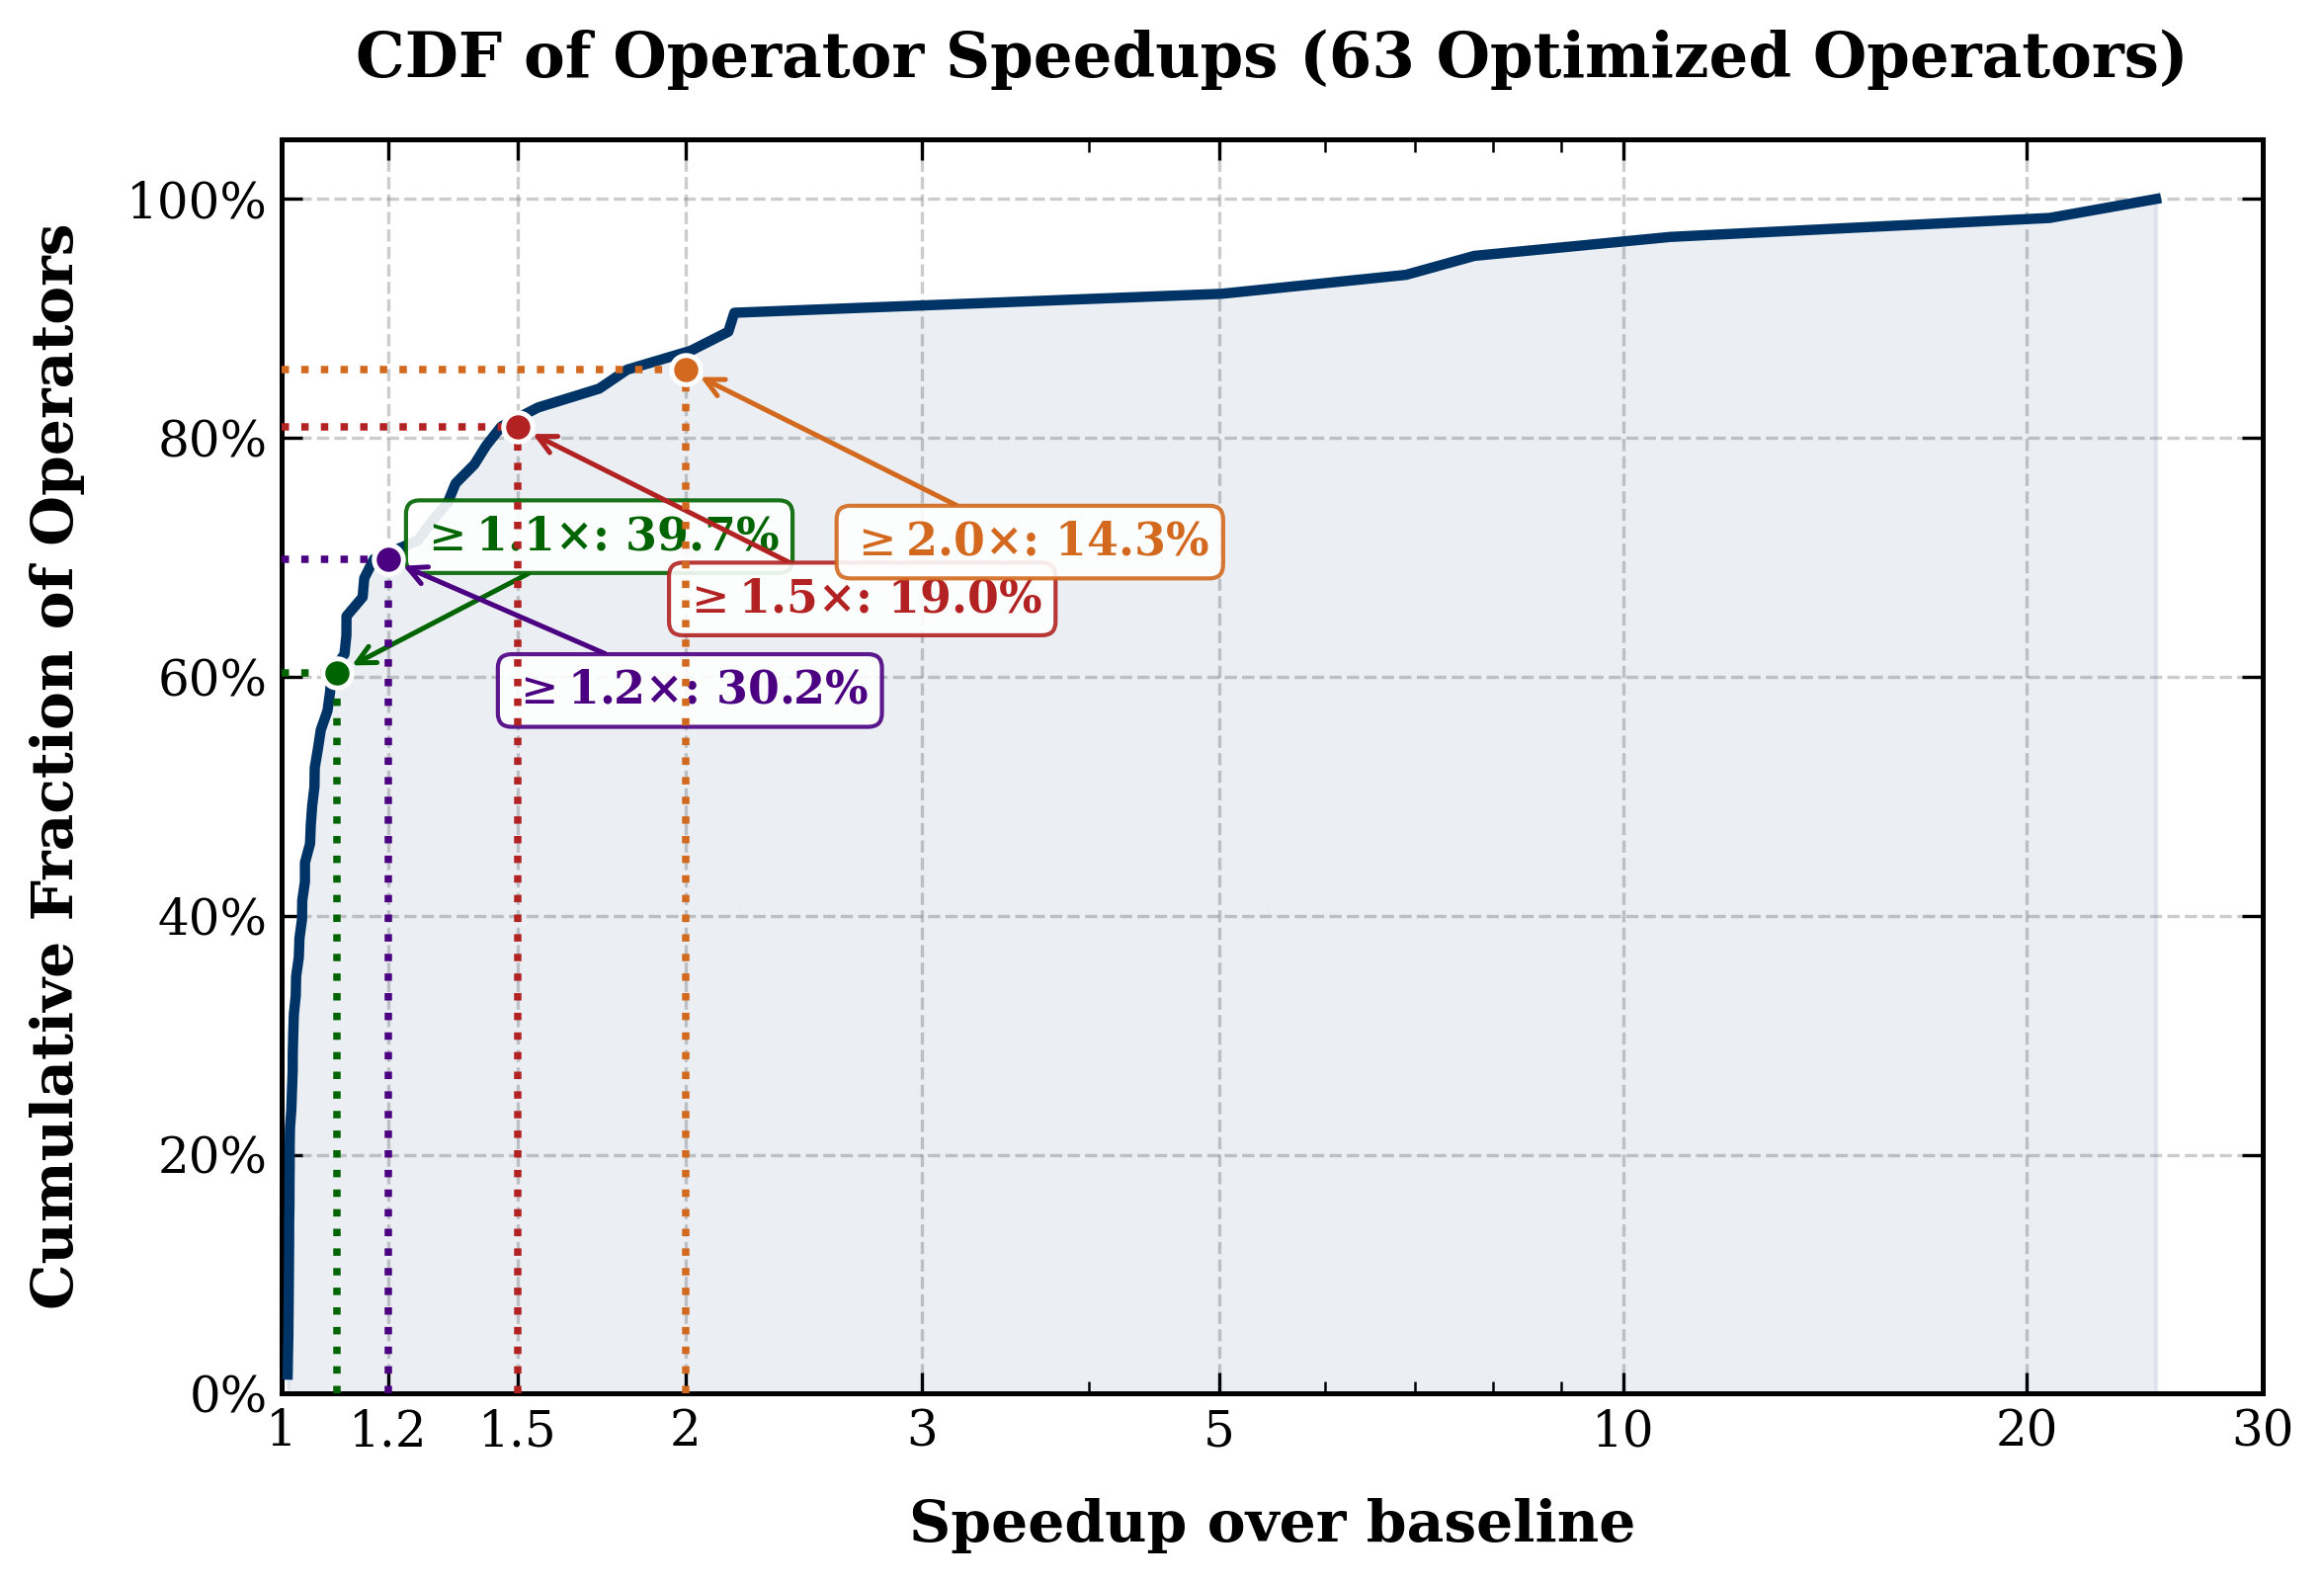
\includegraphics[width=0.64\linewidth]{fig/speedup_distribution.png}
  \caption{CDF of per-operator speedups achieved by \textbf{AscendOptimizer} on 63 optimized operators. The x-axis is the speedup over the baseline and the y-axis is the cumulative fraction of operators. Dashed markers highlight the corresponding tail ratios: \SI{39.7}{\percent} of operators achieve at least $1.1\times$, \SI{30.2}{\percent} achieve at least $1.2\times$, \SI{19.0}{\percent} achieve at least $1.5\times$, and \SI{14.3}{\percent} achieve at least $2.0\times$.}
  \label{fig:improvement}
\end{figure}


\noindent\textbf{Speedup distribution.}
Figure~\ref{fig:improvement} complements the aggregate metrics in Table~\ref{tab:main_performance} by showing the full distribution of improvements. The curve rises rapidly near $1.0\times$--$1.2\times$, indicating that many operators obtain reliable moderate gains, while the long right tail shows that a non-trivial subset benefits from large improvements (up to above $20\times$). In particular, \SI{30.2}{\percent} and \SI{14.3}{\percent} of operators surpass the stricter $1.2\times$ and $2.0\times$ thresholds, respectively, confirming that the method improves both broad coverage and high-end acceleration.

% \noindent\textbf{Optimization dynamics.}
% Figure~\ref{fig:improvement} tracks the evolution of $\mathrm{fast}_p$ over 40 optimization steps, where we alternate every 10 iterations between Stage \Rmnum{1} (tiling/execution parameter tuning) and Stage \Rmnum{2}(experience-bank-driven kernel rewriting).
% The results suggest that Stage \Rmnum{1} primarily improves \emph{coverage}: it quickly increases the number of operators surpassing the baseline, producing higher-quality candidate implementations and providing a stronger starting point for subsequent optimization.
% In contrast, Stage \Rmnum{2} alleviates structural bottlenecks via semantic rewrites and more steadily pushes higher-threshold metrics (e.g., $\mathrm{fast}_{1.2}$, $\mathrm{fast}_{1.4}$, and $\mathrm{fast}_{2.0}$).
% Moreover, the periodic return to Stage \Rmnum{1} further squeezes the remaining tuning headroom and helps converge and validate configurations for the rewritten implementations.
% Figure~\ref{fig:improvement} illustrates the evolution of $\mathrm{fast}_p$ over 40 steps. The results indicate that Stage \Rmnum{1} (tiling and parameter tuning) primarily enhances coverage by quickly identifying implementations that surpass the baseline. Stage \Rmnum{2} (experience-driven rewriting) addresses structural bottlenecks through semantic changes, steadily improving the higher-threshold metrics. The periodic alternation between these stages allows the system to exhaust remaining tuning potential while validating rewritten code, creating a continuous improvement loop rather than a simple additive effect.


% \begin{figure*}[htbp]
% \centering
% 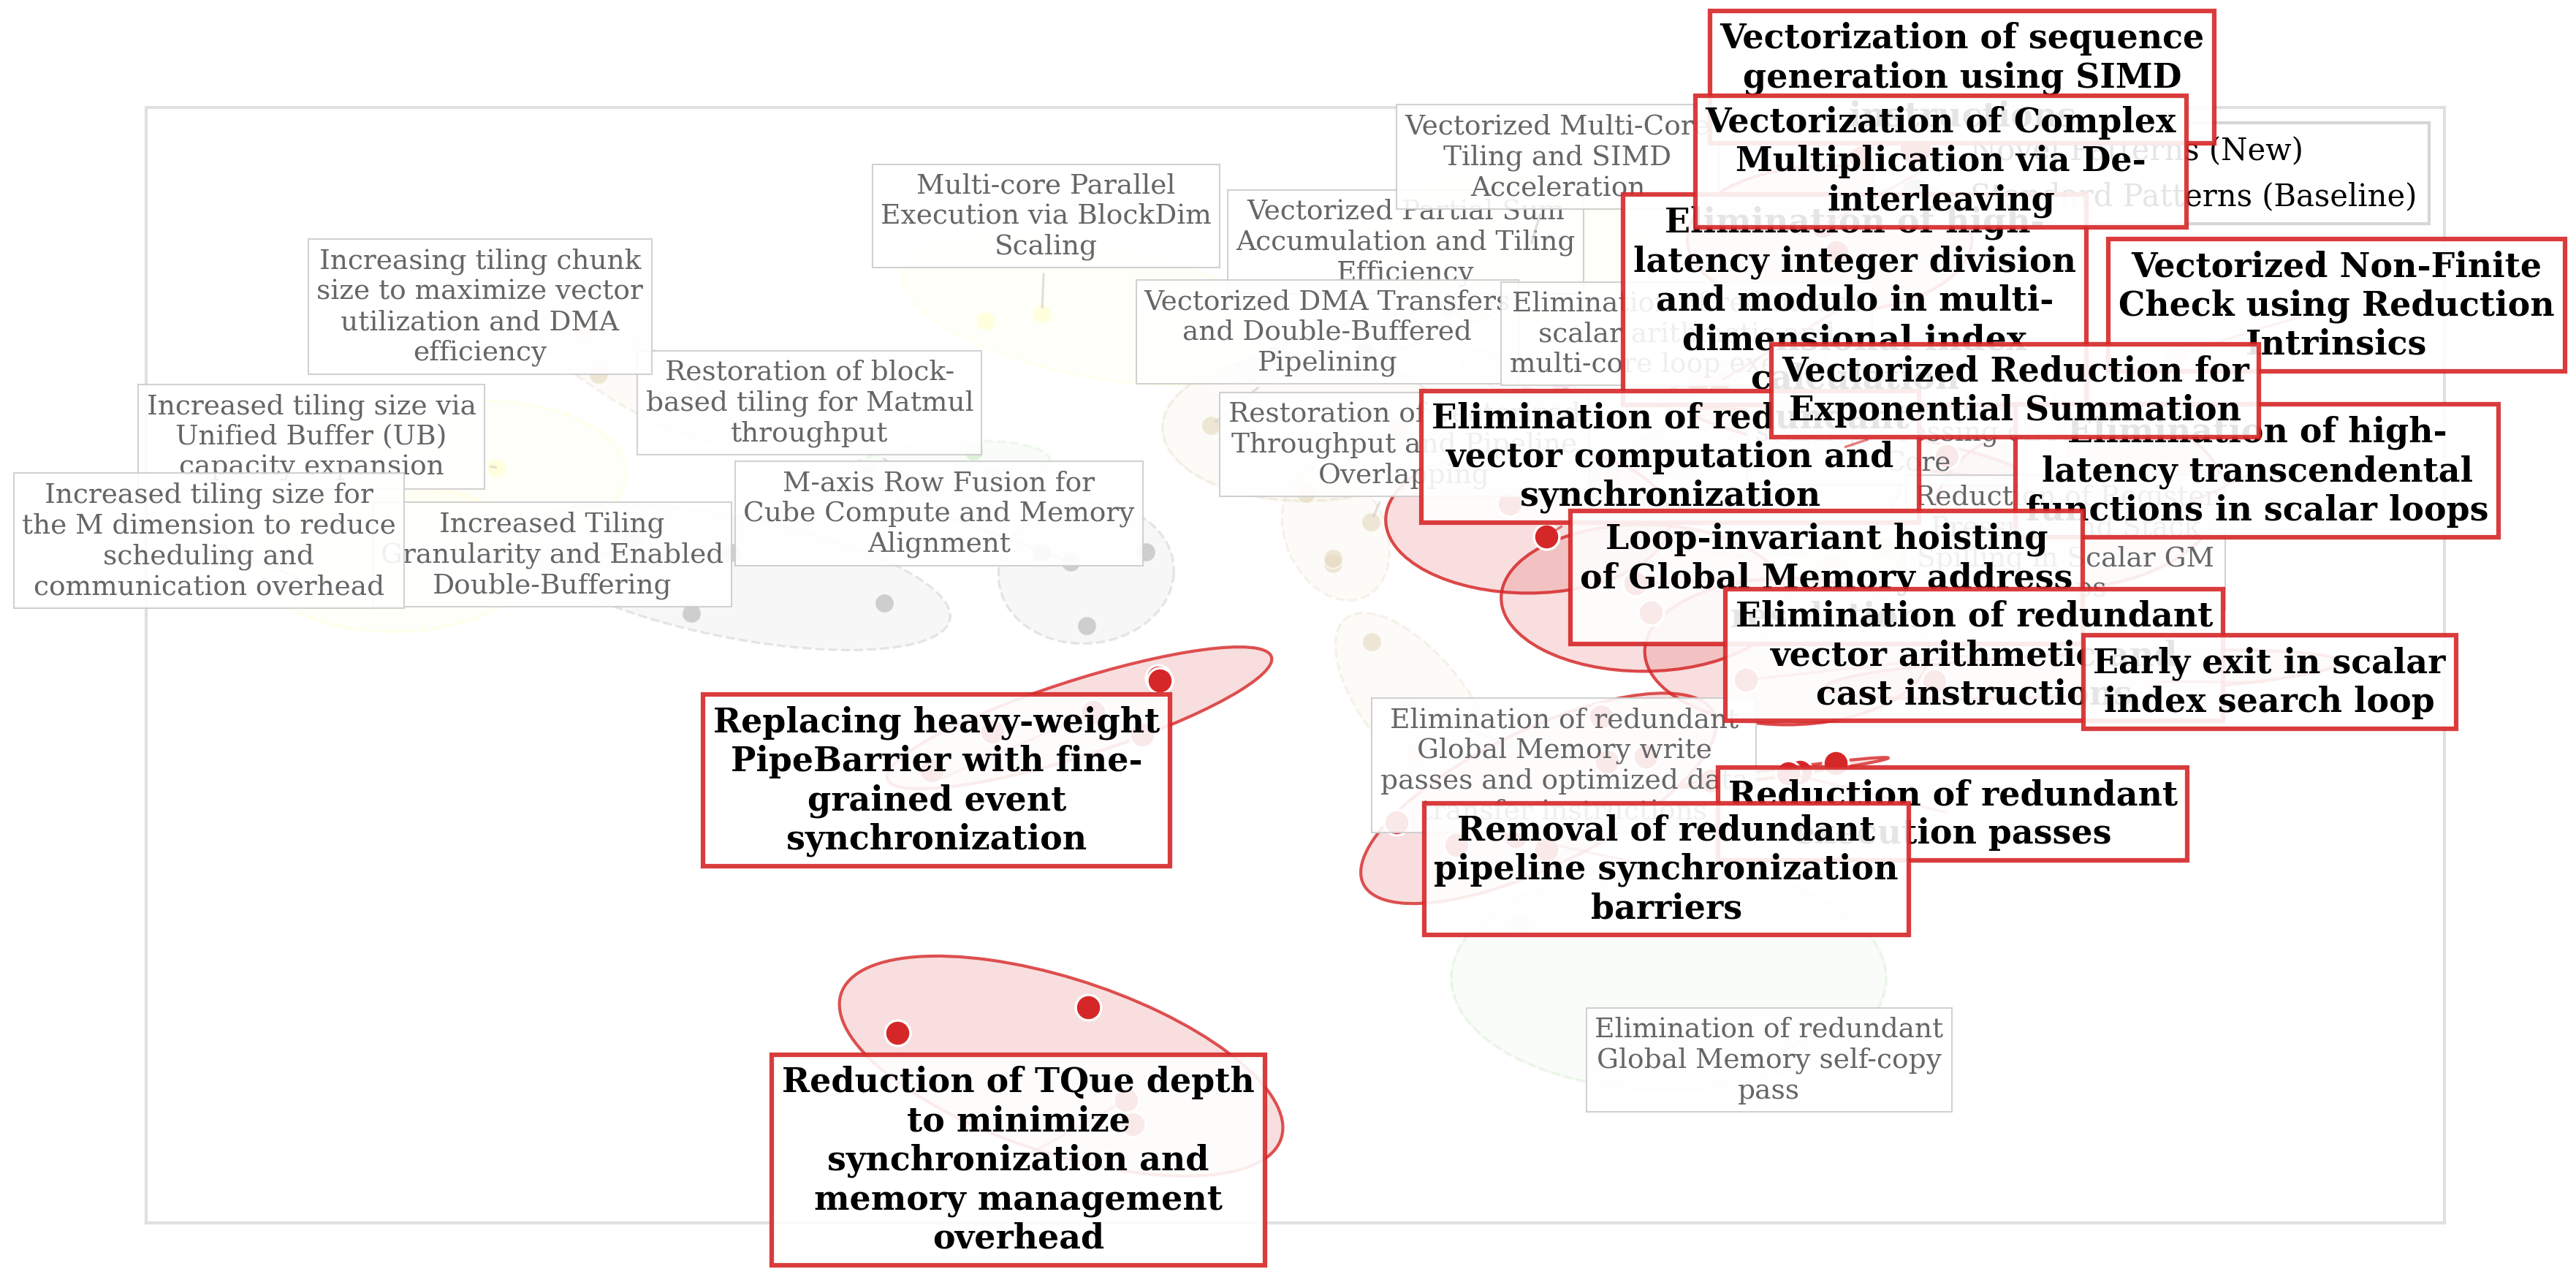
\includegraphics[width=0.65\textwidth]{fig/cluster_scatter_llm.png}
% \caption{Semantic landscape of optimization strategies via embedding clustering.
% Each optimization record (Title \& Description) is embedded using an embedding model, projected to 2D for visualization with PCA, and clustered with K-Means.
% Grey/light regions denote clusters aligned with categories described in the official documentation, while red regions denote clusters that do not directly correspond to the documentation’s explicit taxonomy.}
% \label{fig:semantic_landscape}
% \end{figure*}
% Overall, the figure indicates that the alternating strategy is not a simple additive combination of two techniques: Stage \Rmnum{1} provides stable and efficient low-level tuning, while Stage \Rmnum{2} enables structural rewrites that break performance ceilings, and their alternation forms a continuously progressing optimization loop.
% \begin{figure}[htbp]
%   \centering
%   \includegraphics[width=\linewidth]{fig/optimization_improvement_curve.png}
%   \caption{Optimization dynamics over 40 steps: alternating Stage \Rmnum{1} tiling/execution tuning and Stage \Rmnum{2} experience-bank-driven kernel optimization, tracked by $\mathrm{fast}_p$ across thresholds.}
%   \label{fig:improvement}
% \end{figure}



% TODO:Add real shape optimization
% \begin{figure}[htbp]
%   \centering
%   \begin{tikzpicture}
%     % 柱状图
%   \end{tikzpicture}
%   \caption{TODO:Flash Infer Bench Shape Optimization}
%   \label{fig:placeholder}
% \end{figure}


\subsection{Ablation Study}

% We conduct an ablation study to quantify the contribution of each component in \textsc{AscendOptimizer}, with all baselines implemented as \textsc{EvoAscend} variants (\Cref{tab:ablation_performance}). Stage \Rmnum{1} (low-level tiling/execution tuning) already improves the coarse metric fast$_{1.0}$ to \SI{40.60}{\percent} but struggles on higher-threshold metrics (e.g., fast$_{2.0}$=\SI{5.26}{\percent}), indicating limited ability to break structural performance ceilings. Stage \Rmnum{2} introduces semantic kernel rewrites and achieves a clear gain on mid-threshold speedups (fast$_{1.2}$=\SI{18.80}{\percent} vs.\ \SI{9.02}{\percent} in Stage \Rmnum{1}), while its high-threshold improvement remains limited in this setting (fast$_{2.0}$=\SI{6.02}{\percent}). Combining both stages via the full \textsc{AscendOptimizer} achieves the best overall performance, improving GM to 1.34 and fast$_{1.0}$ to \SI{51.88}{\percent}, while also retaining strong high-threshold results (fast$_{2.0}$=\SI{12.03}{\percent}). Overall, the results suggest that Stage \Rmnum{1} provides robust low-level efficiency, Stage \Rmnum{2} contributes complementary semantic rewrites that raise higher-threshold metrics, and their alternation yields cumulative gains beyond either stage alone.
We evaluate the contribution of each component within \textsc{AscendOptimizer}, as shown in \Cref{tab:ablation_performance}. To ensure a fair comparison, all configurations are evaluated under the same optimization budget. Stage \Rmnum{1} alone yields a GM of 1.09, with fast$_{1.0}$ at \SI{38.58}{\percent} and fast$_{2.0}$ at \SI{3.15}{\percent}, indicating that tiling/execution tuning improves robustness but has limited headroom at stricter speedup thresholds. Stage \Rmnum{2} alone improves GM to 1.12 and achieves the best mid-threshold metrics (fast$_{1.2}$=\SI{15.75}{\percent}, fast$_{1.4}$=\SI{11.81}{\percent}), showing the benefit of semantic kernel rewriting. The full \textsc{AscendOptimizer} obtains the best overall trade-off, with the highest GM (1.19), the highest fast$_{1.0}$ (\SI{49.61}{\percent}), and the highest fast$_{2.0}$ (\SI{7.09}{\percent}). These results suggest that Stage \Rmnum{1} and Stage \Rmnum{2} are complementary, and alternating them is important for jointly improving average gains and high-threshold acceleration.

\begin{table}[!t]
\centering

\caption{Ablation results of \textsc{AscendOptimizer}. All rows are \textsc{EvoAscend} variants. Higher is better ($\uparrow$). Fast is reported in \% (shown once in the header).}
\label{tab:ablation_performance}
\setlength{\tabcolsep}{3pt}
\begin{tabular}{@{}l c c c c c@{}}
\toprule
\textbf{Variant} & \textbf{GM} $\uparrow$ &
\multicolumn{4}{c}{\textbf{fast$_p$} (\%, $\uparrow$)} \\
\cmidrule(l){3-6}
 &  & \textbf{p=1.0} & \textbf{p=1.2} & \textbf{p=1.4} & \textbf{p=2.0} \\
\midrule
stage \Rmnum{1}  & 1.09 & 38.58    & 7.09  & 4.72    & 3.15   \\
% stage \Rmnum{2} w/o Skill  & 1.20   & 35.34    & 16.54    & 15.79    & 12.03   \\
stage \Rmnum{2}     & 1.12    & 37.80   & \textbf{15.75}   & \textbf{11.81}    & 4.72
\\
\midrule
\textbf{AscendOptimizer (Ours)} & \textbf{1.19} & \textbf{49.61} & 14.96 & 11.02 & \textbf{7.09} \\
\bottomrule
\end{tabular}
\end{table}

% \subsubsection{Without Thought}
% TODO:加没有优化经验、不使用tiling搜索的消融结果.
% TODO: The ablation results without optimization experience and without using tiling search.
% \begin{table}[htbp]
% \centering
% \renewcommand{\arraystretch}{1.5}
% \renewcommand{\arraystretch}{1.2}
% \begin{tabularx}{\columnwidth}{|c|c|c|c|c|c|c|}
% \hline
% Method & GM & Fast$_{1.0}$ & Fast$_{1.2}$ & Fast$_{1.4}$ &  Fast$_{2.0}$ \\ \hline
% EvoAscend w/o tiling &   &  &  &  &  \\ \hline
% EvoAscend w/o thought &   &  &  &  &  \\ \hline
% EvoAscend w/o rag &   &  &  &  &  \\ \hline
% EvoAscend & 1.50 & 46.62\% & 16.54\% & 12.78\% & 9.02\% \\ \hline
% \end{tabularx}
% \caption{ ablation\_performance}
% \end{table}

% Suggested packages:
% \usepackage{booktabs}
% \usepackage{tabularx}

% Suggested packages:
% \usepackage{booktabs}
% \usepackage{tabularx}

% Suggested packages:
% \usepackage{booktabs}
% \usepackage{tabularx}

% Suggested packages:
% \usepackage{booktabs}
% \usepackage{tabularx}

% \begin{table}[t]
% \centering

% \caption{Ablation results of \textsc{EvoAscend}. All rows are \textsc{EvoAscend} variants. Higher is better ($\uparrow$). Fast is reported in \% (shown once in the header).}
% \label{tab:ablation_performance}
% \begin{tabularx}{\columnwidth}{@{}l c c c c c@{}}
% \toprule
% \textbf{Variant} & \textbf{GM} $\uparrow$ &
% \multicolumn{4}{c}{\textbf{fast$_p$} (\%, $\uparrow$)} \\
% \cmidrule(l){3-6}
%  &  & \textbf{p=1.0} & \textbf{p=1.2} & \textbf{p=1.4} & \textbf{p=2.0} \\
% \midrule
% % w/o tiling  & --   & --    & --    & --    & --   \\
% % w/o thought & --   & --    & --    & --    & --   \\
% w/o Skill     & 1.80    & 42.11    & 18.80    & 15.04    & 13.53
% \\
% \midrule
% \textbf{Full (Ours)} & \textbf{1.50} & \textbf{46.62} & \textbf{16.54} & \textbf{12.78} & \textbf{9.02} \\
% \bottomrule
% \end{tabularx}
% \end{table}





\subsection{Case Study}
\subsubsection{Semantic Analysis of the Experience Bank}


% \paragraph{Semantic organization of optimization strategies.}
To further analyze how optimization experience is organized in the experience bank, Figure~\ref{fig:semantic_landscape} visualizes the semantic distribution of optimization instances extracted from the bank.
Concretely, we encode each optimization record (Title and Description) into a vector representation, and apply dimensionality reduction and clustering to reveal how different strategy families group in the semantic space.


\begin{figure}[htbp]
\centering
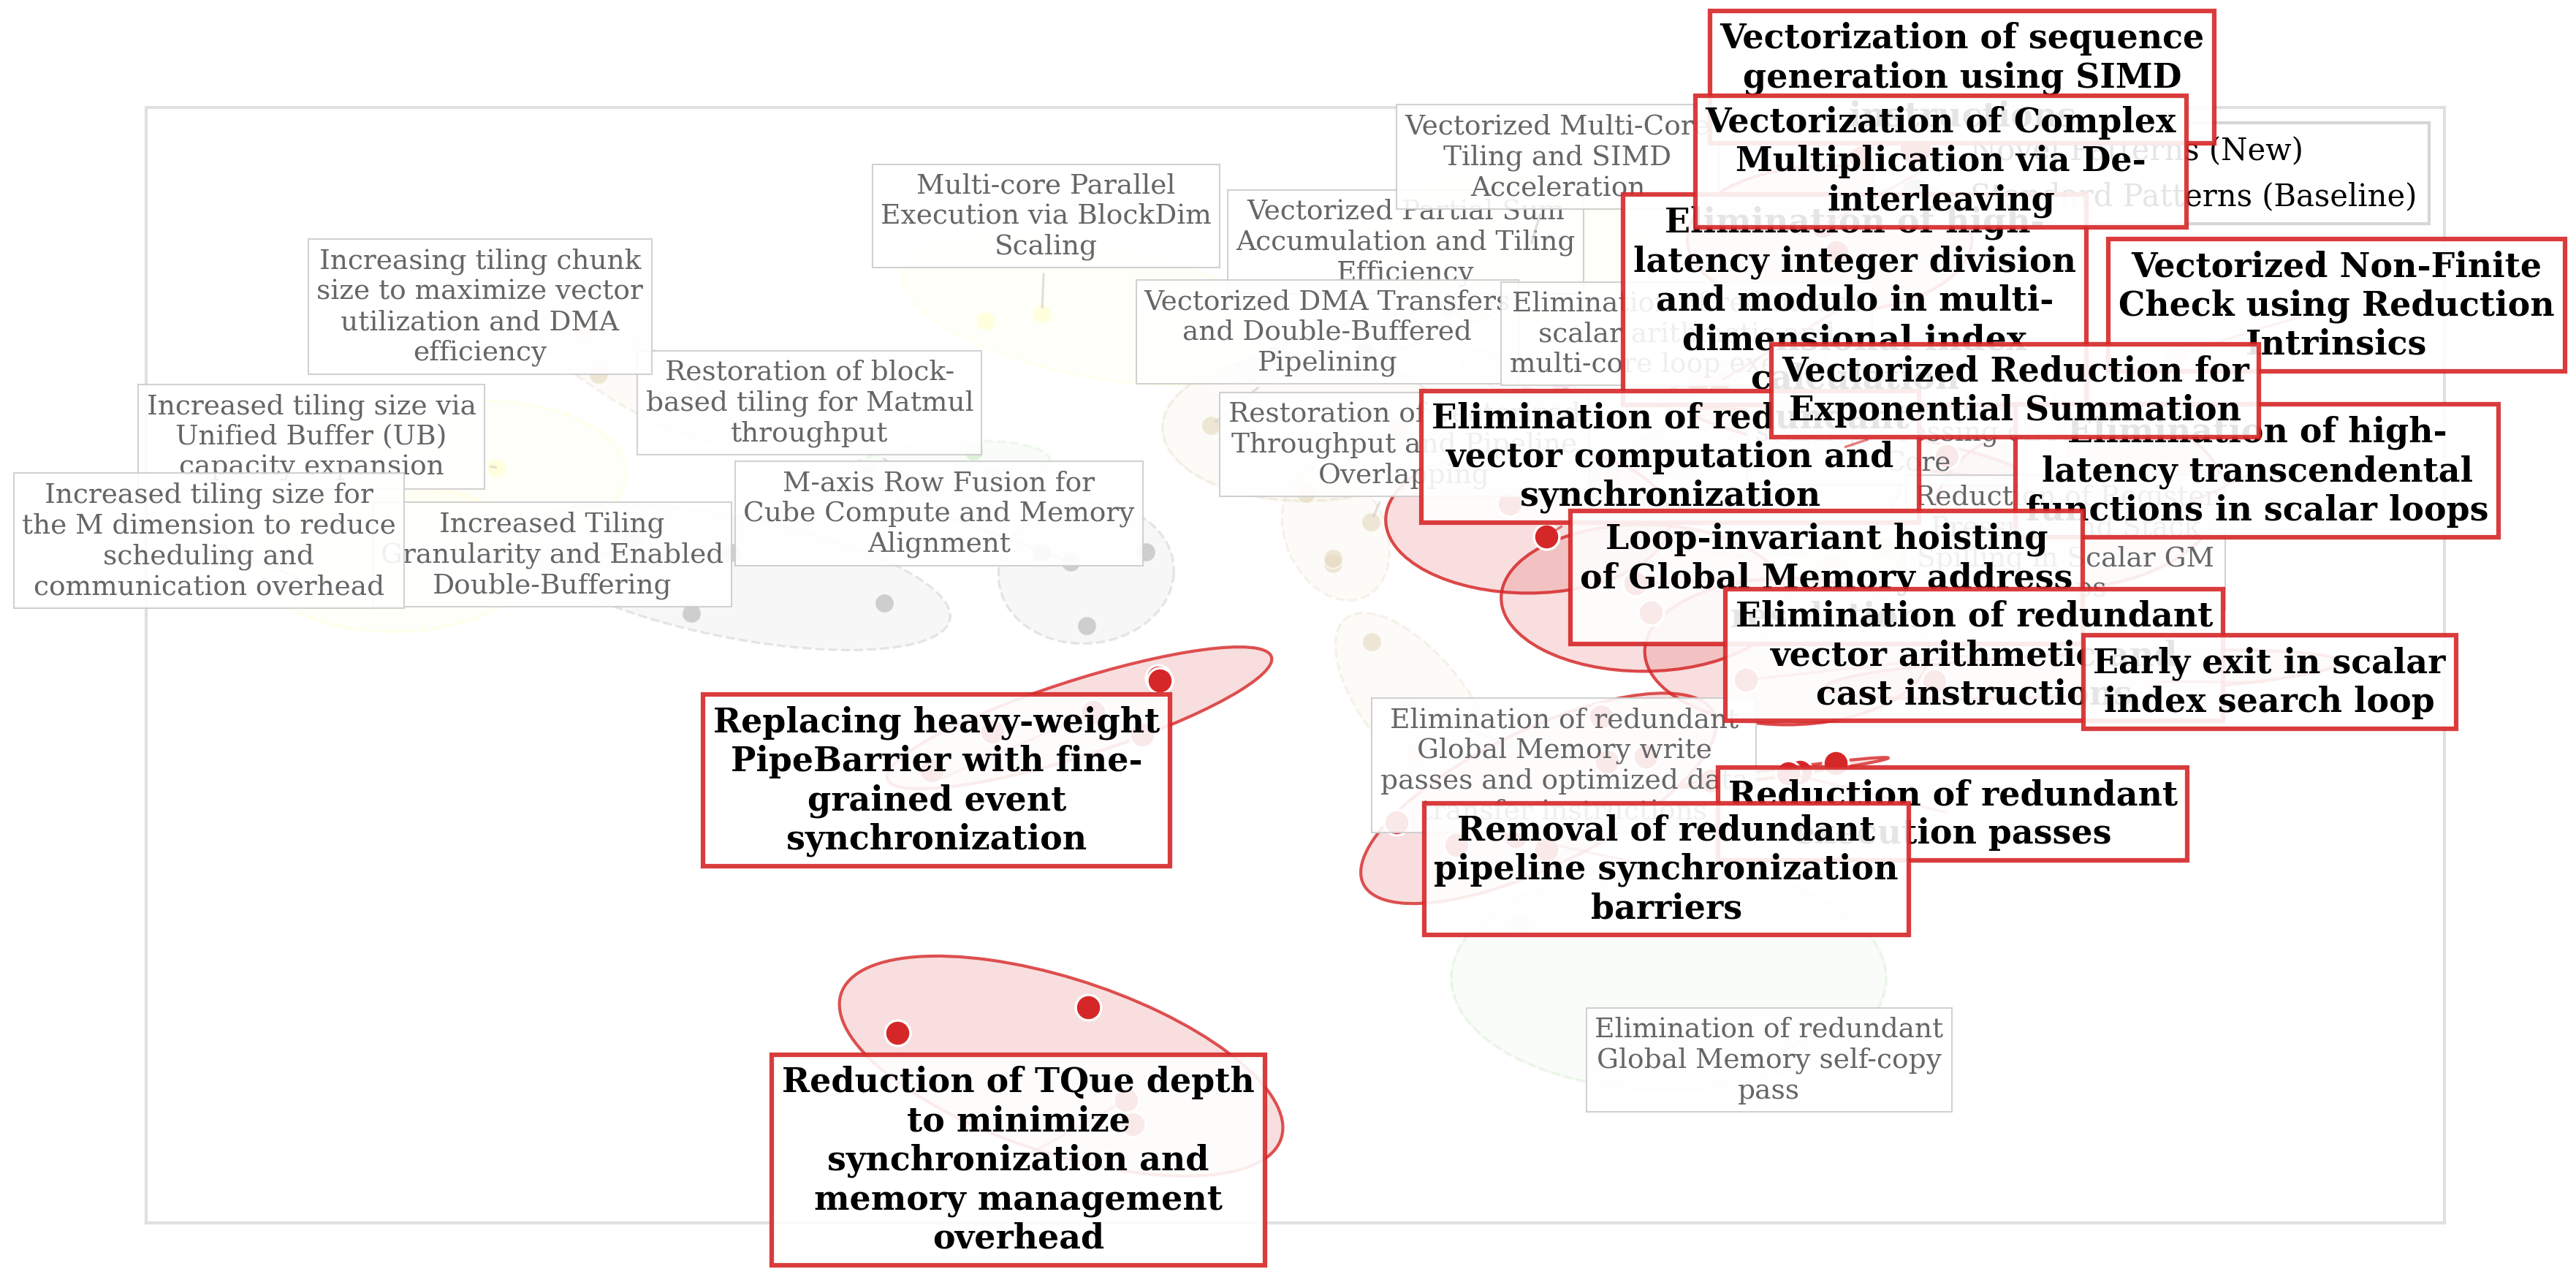
\includegraphics[width=0.88\linewidth]{fig/cluster_scatter_llm.png}
\caption{Semantic landscape of optimization strategies via embedding clustering.
Each optimization record (Title \& Description) is embedded using an embedding model, projected to 2D for visualization with PCA, and clustered with K-Means.
Grey/light regions denote clusters aligned with categories described in the official documentation, while red regions denote clusters that do not directly correspond to the documentation’s explicit taxonomy.}
\label{fig:semantic_landscape}
\end{figure}

As shown in Figure~\ref{fig:semantic_landscape}, the strategies produced by AscendOptimizer form compact and separable clusters in the embedding space.
Some clusters align with best-practice categories described in the official documentation (e.g., tiling adjustments and double buffering; shaded in grey).
Meanwhile, we also observe several clusters that do not map cleanly to the documentation’s explicit taxonomy (highlighted in red).
These clusters include patterns such as finer-grained event synchronization, vectorized non-finite checks, and elimination of high-latency scalar instructions.
The figure suggests that the experience bank captures not only common, standard optimization strategies, but also recurring patterns that emerge in practice yet are not explicitly categorized in the official documentation.





% \begin{table*}[t]
% \centering
% \caption{Validation and Extension of Official Ascend C Best Practices by the Optimization Experience Bank}
% \label{tab:validation_extension}
% \begin{tabular}{p{3.6cm} p{2.6cm} p{2.6cm} p{5.0cm} p{2.4cm}}
% \toprule
% % \samll
% \textbf{Optimization Category}
% & \textbf{Covered in Docs}
% & \textbf{Doc Granularity}
% & \textbf{Observed Optimization Behavior}
% & \textbf{Relation} \\
% \midrule
% Tiling granularity and arithmetic intensity
% & Yes
% & High-level principle
% & Dimension-aware tiling adjustments under Unified Buffer capacity constraints
% & Validation + refinement \\

% Double buffering and pipeline parallelism
% & Yes
% & Mechanism-level
% & Conditional enabling of double buffering coordinated with tile size
% & Validation + conditionalization \\

% Reduction of GM--UB redundant transfers
% & Yes
% & Qualitative
% & Elimination of redundant data transfers and consolidation of memory operations
% & Validation + structuring \\

% Vectorization and SIMD utilization
% & Yes
% & Principle-level
% & Vectorized reduction, SIMD branch elimination, and replacement of scalar loops
% & Validation + extension \\

% Synchronization and barrier overhead reduction
% & Partial
% & Scattered
% & Fine-grained synchronization replacement and queue depth tuning
% & Supplementing implicit experience \\

% Scalar arithmetic and index computation optimization
% & No
% & --
% & Elimination of high-latency scalar arithmetic and simplification of index computation
% & Undocumented \\

% Elimination of scalar-path interference on AI Core
% & No
% & --
% & Removal of serial scalar execution and early termination of scalar search paths
% & Undocumented \\
% \bottomrule
% \end{tabular}
% \end{table*}
\subsubsection{Operator Optimization Trajectory}
In Stage \Rmnum{2}, the system diagnoses bottlenecks, retrieves relevant patterns, and applies semantic rewrites (e.g., pipelining/synchronization and mapping changes). \Cref{fig:code_diff} illustrates a representative rewrite: we replace the remainder-based per-core quota assignment with block-level load balancing and a nested scan across tensors, which reduces tail imbalance and improves core utilization. Correspondingly, a major jump at iteration 33 (within a Stage \Rmnum{2} period) introduces a more effective heterogeneous core mapping and reaches $\num{2.31}\times$.

\begin{figure}[H]
  \centering
  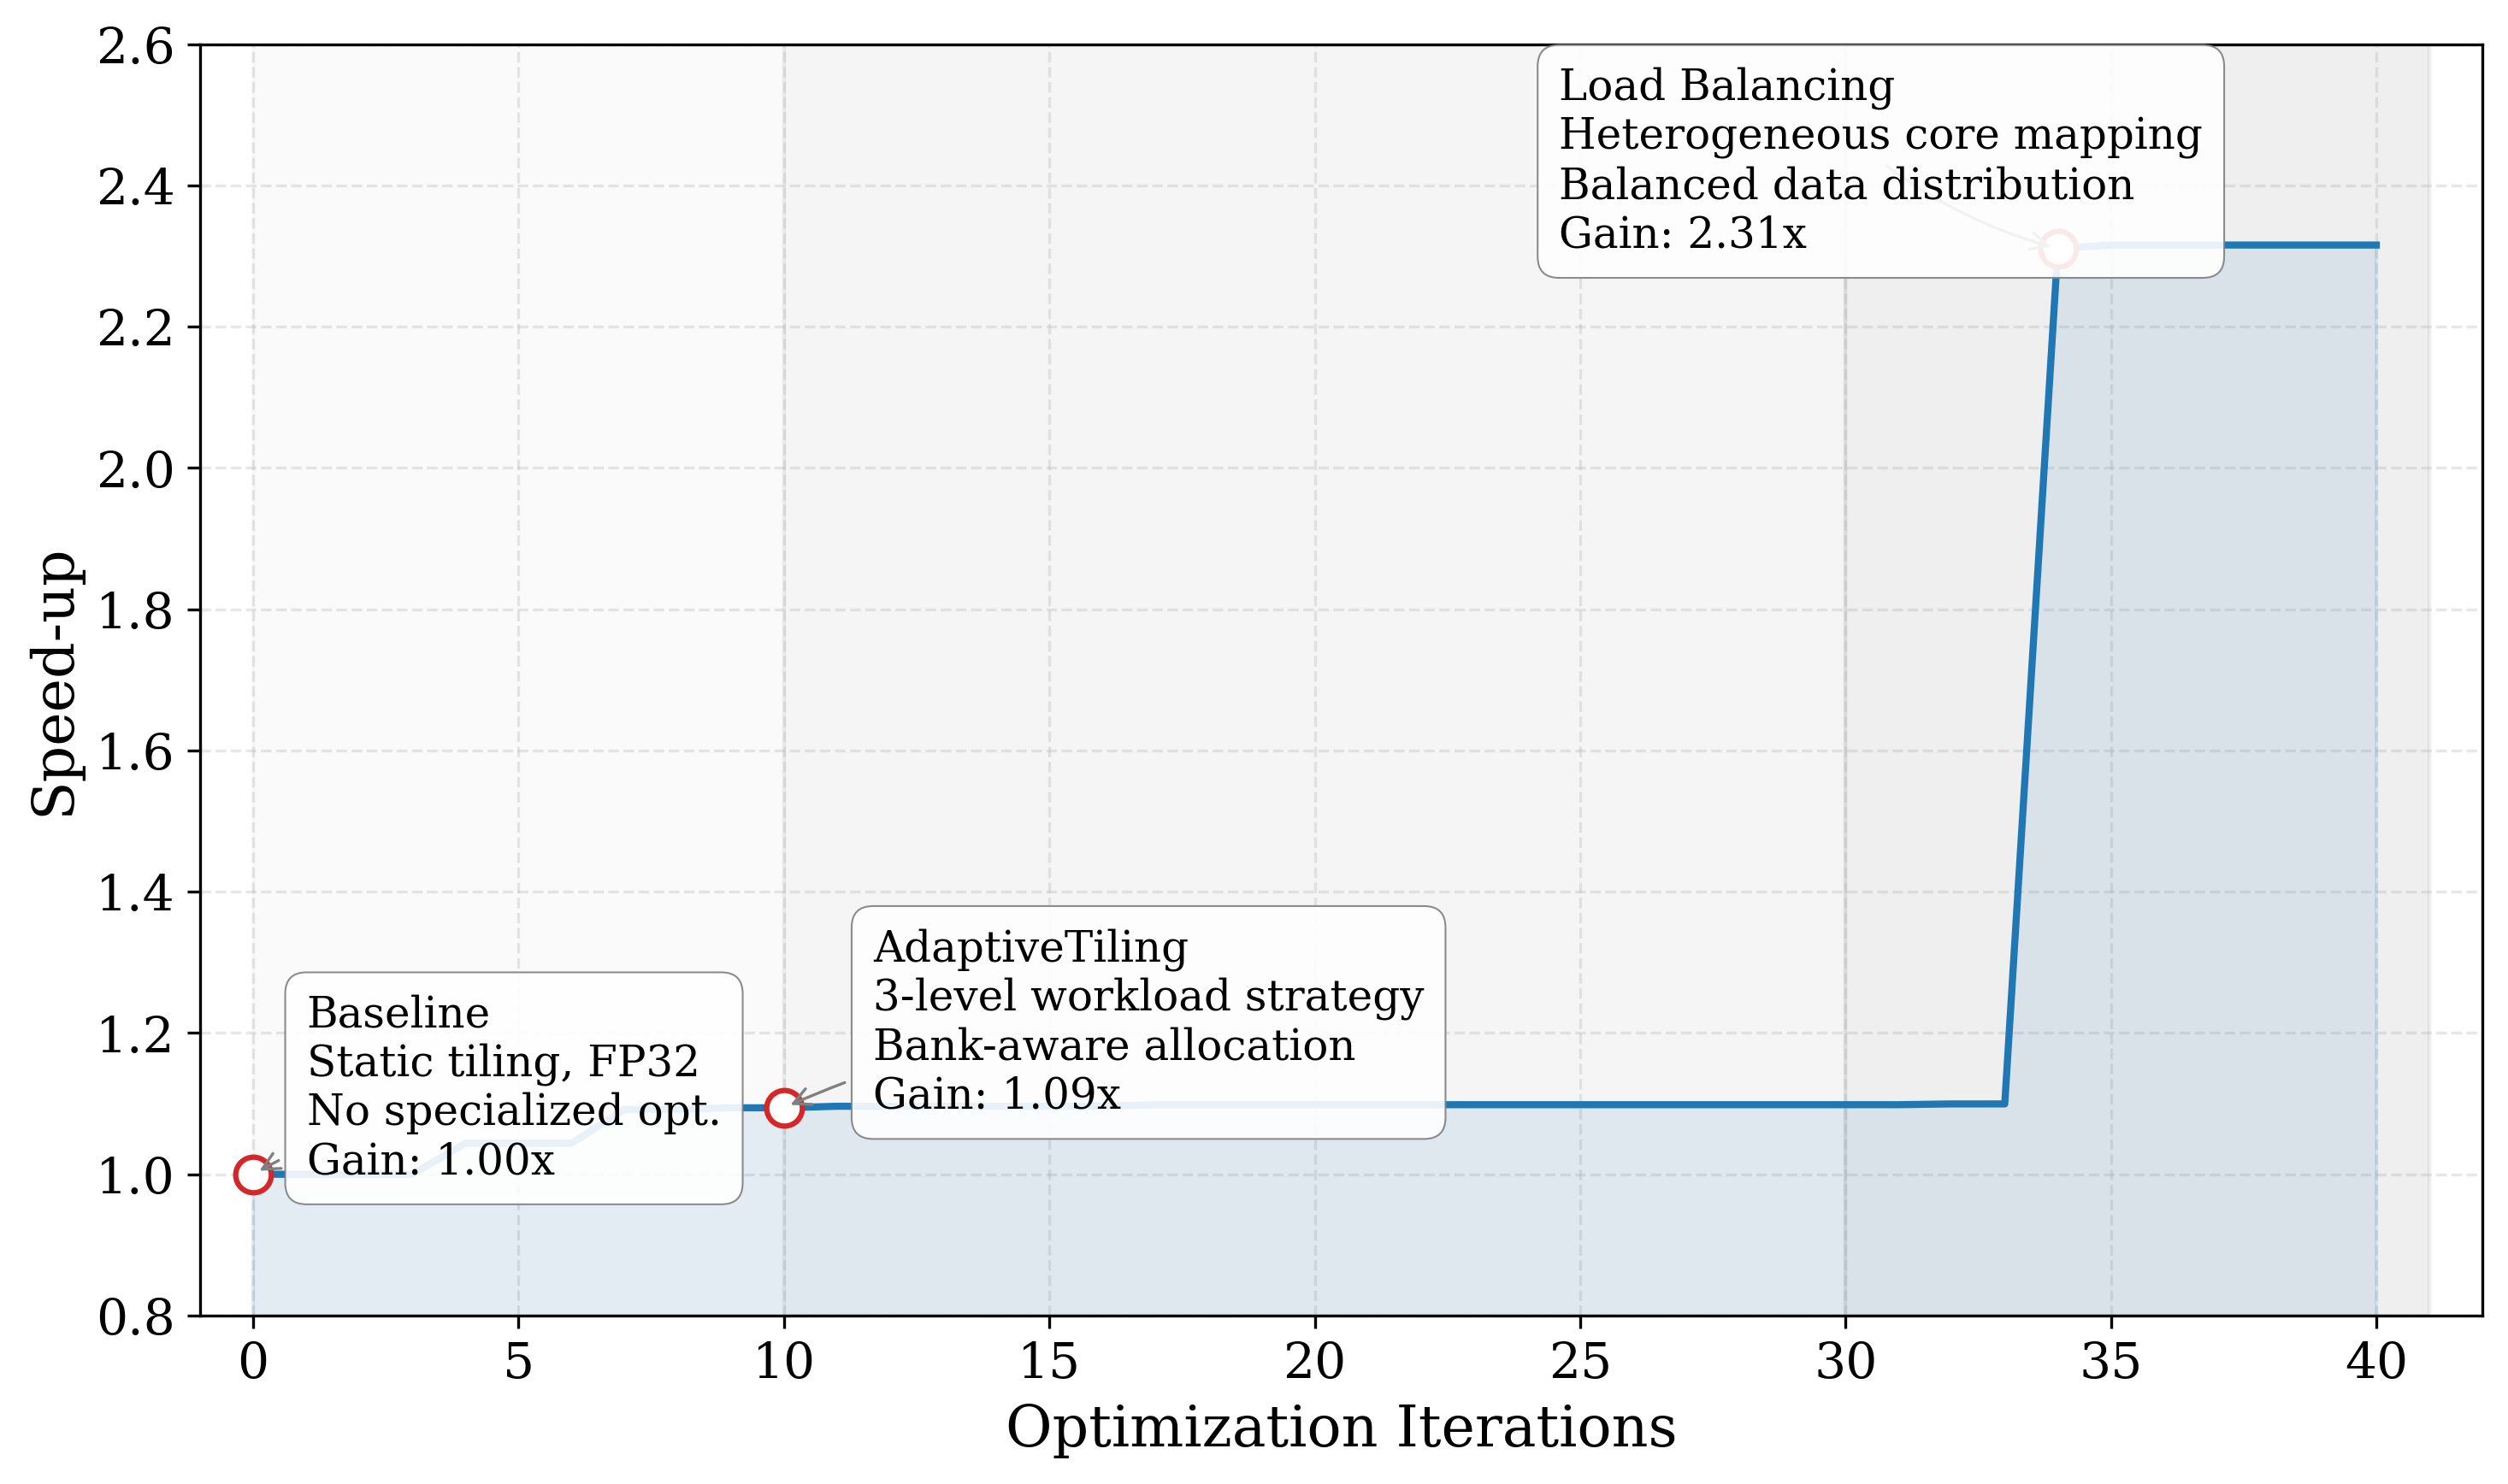
\includegraphics[width=0.62\linewidth]{fig/single_ops_curve.png}
  \caption{Optimization trajectory of the "foreach\_pow\_scalar\_and\_tensor" operator.}
  \label{fig:single_op_curve}
\end{figure}


\lstset{
  basicstyle=\ttfamily\small,
  columns=fullflexible,
  keepspaces=true,
  showstringspaces=false,
  frame=none,
  breaklines=true,
  breakatwhitespace=true,
  escapeinside={(*@}{@*)}
}

% \begin{figure}[t]
% \centering
% {\lstset{basicstyle=\ttfamily\scriptsize,
%   columns=fullflexible,
%   keepspaces=true,
%   showstringspaces=false,
%   frame=none,
%   breaklines=true,
%   breakatwhitespace=true,
%   escapeinside={(*@}{@*)}}
% \begin{tikzpicture}[
%   box/.style={
%     draw=black!50,
%     rounded corners=2pt,
%     inner sep=5pt,
%     align=left,
%     text width=0.43\linewidth,
%     fill=black!1
%   },
%   >={Stealth[length=2.2mm]}
% ]

% % ---------- (a) Original ----------
% \node[box] (A) {
% \textbf{(a) Original: remainder-based per-core quota}\par\medskip
% \begin{lstlisting}
% blockCount = ceil(totalData / elemsPerBlock)
% baseElems  = (blockCount / nCores) * elemsPerBlock
% remBlocks  =  blockCount % nCores

% for core in [0 .. nCores-1]:
%   quota[core] = baseElems
%   if core < remBlocks:
%     quota[core] += elemsPerBlock   // +1 block

% // assign contiguous ranges to each core
% scan tensors and cut when used == quota[core]
% \end{lstlisting}
% };

% % ---------- (b) Optimized ----------
% \node[box, right=10pt of A] (B) {
% \textbf{(b) Optimized: block-level load balancing (big/small cores)}\par\medskip
% \begin{lstlisting}
% blockCount = ceil(totalData / elemsPerBlock)

% (*@\textcolor{red}{blocksPerCore = blockCount / nCores}@*)
% (*@\textcolor{red}{tailBlocks    = blockCount % nCores}@*)

% for core in [0 .. nCores-1]:
%   (*@\textcolor{red}{coreBlocks = blocksPerCore + (core < tailBlocks)}@*)quota[core] = (*@\textcolor{red}{coreBlocks}@*) * elemsPerBlock

% (*@\textcolor{red}{// nested scan: fill each core's quota across tensors}@*)
% for core in [0 .. nCores-1]:
%   while quota[core] > 0:
%     take = min(quota[core], remaining(tensor))
%     assign(core, tensor, take)
%     quota[core] -= take
% \end{lstlisting}
% };

% ---------- Arrow ----------
% \draw[->, thick] (A.east) -- (B.west);

% \end{tikzpicture}
% }

% \captionsetup{justification=raggedright,singlelinecheck=false}
% \caption{Illustration of a key scheduling rewrite in \texttt{foreach\_\allowbreak pow\_\allowbreak scalar\_\allowbreak and\_\allowbreak tensor}: (a) the original remainder-based per-core quota assignment; (b) the optimized block-level load balancing with a nested scan across tensors (changes highlighted in red).}
% \label{fig:code_diff}
% \end{figure}







% \begin{figure}[htbp]
%   \centering
%   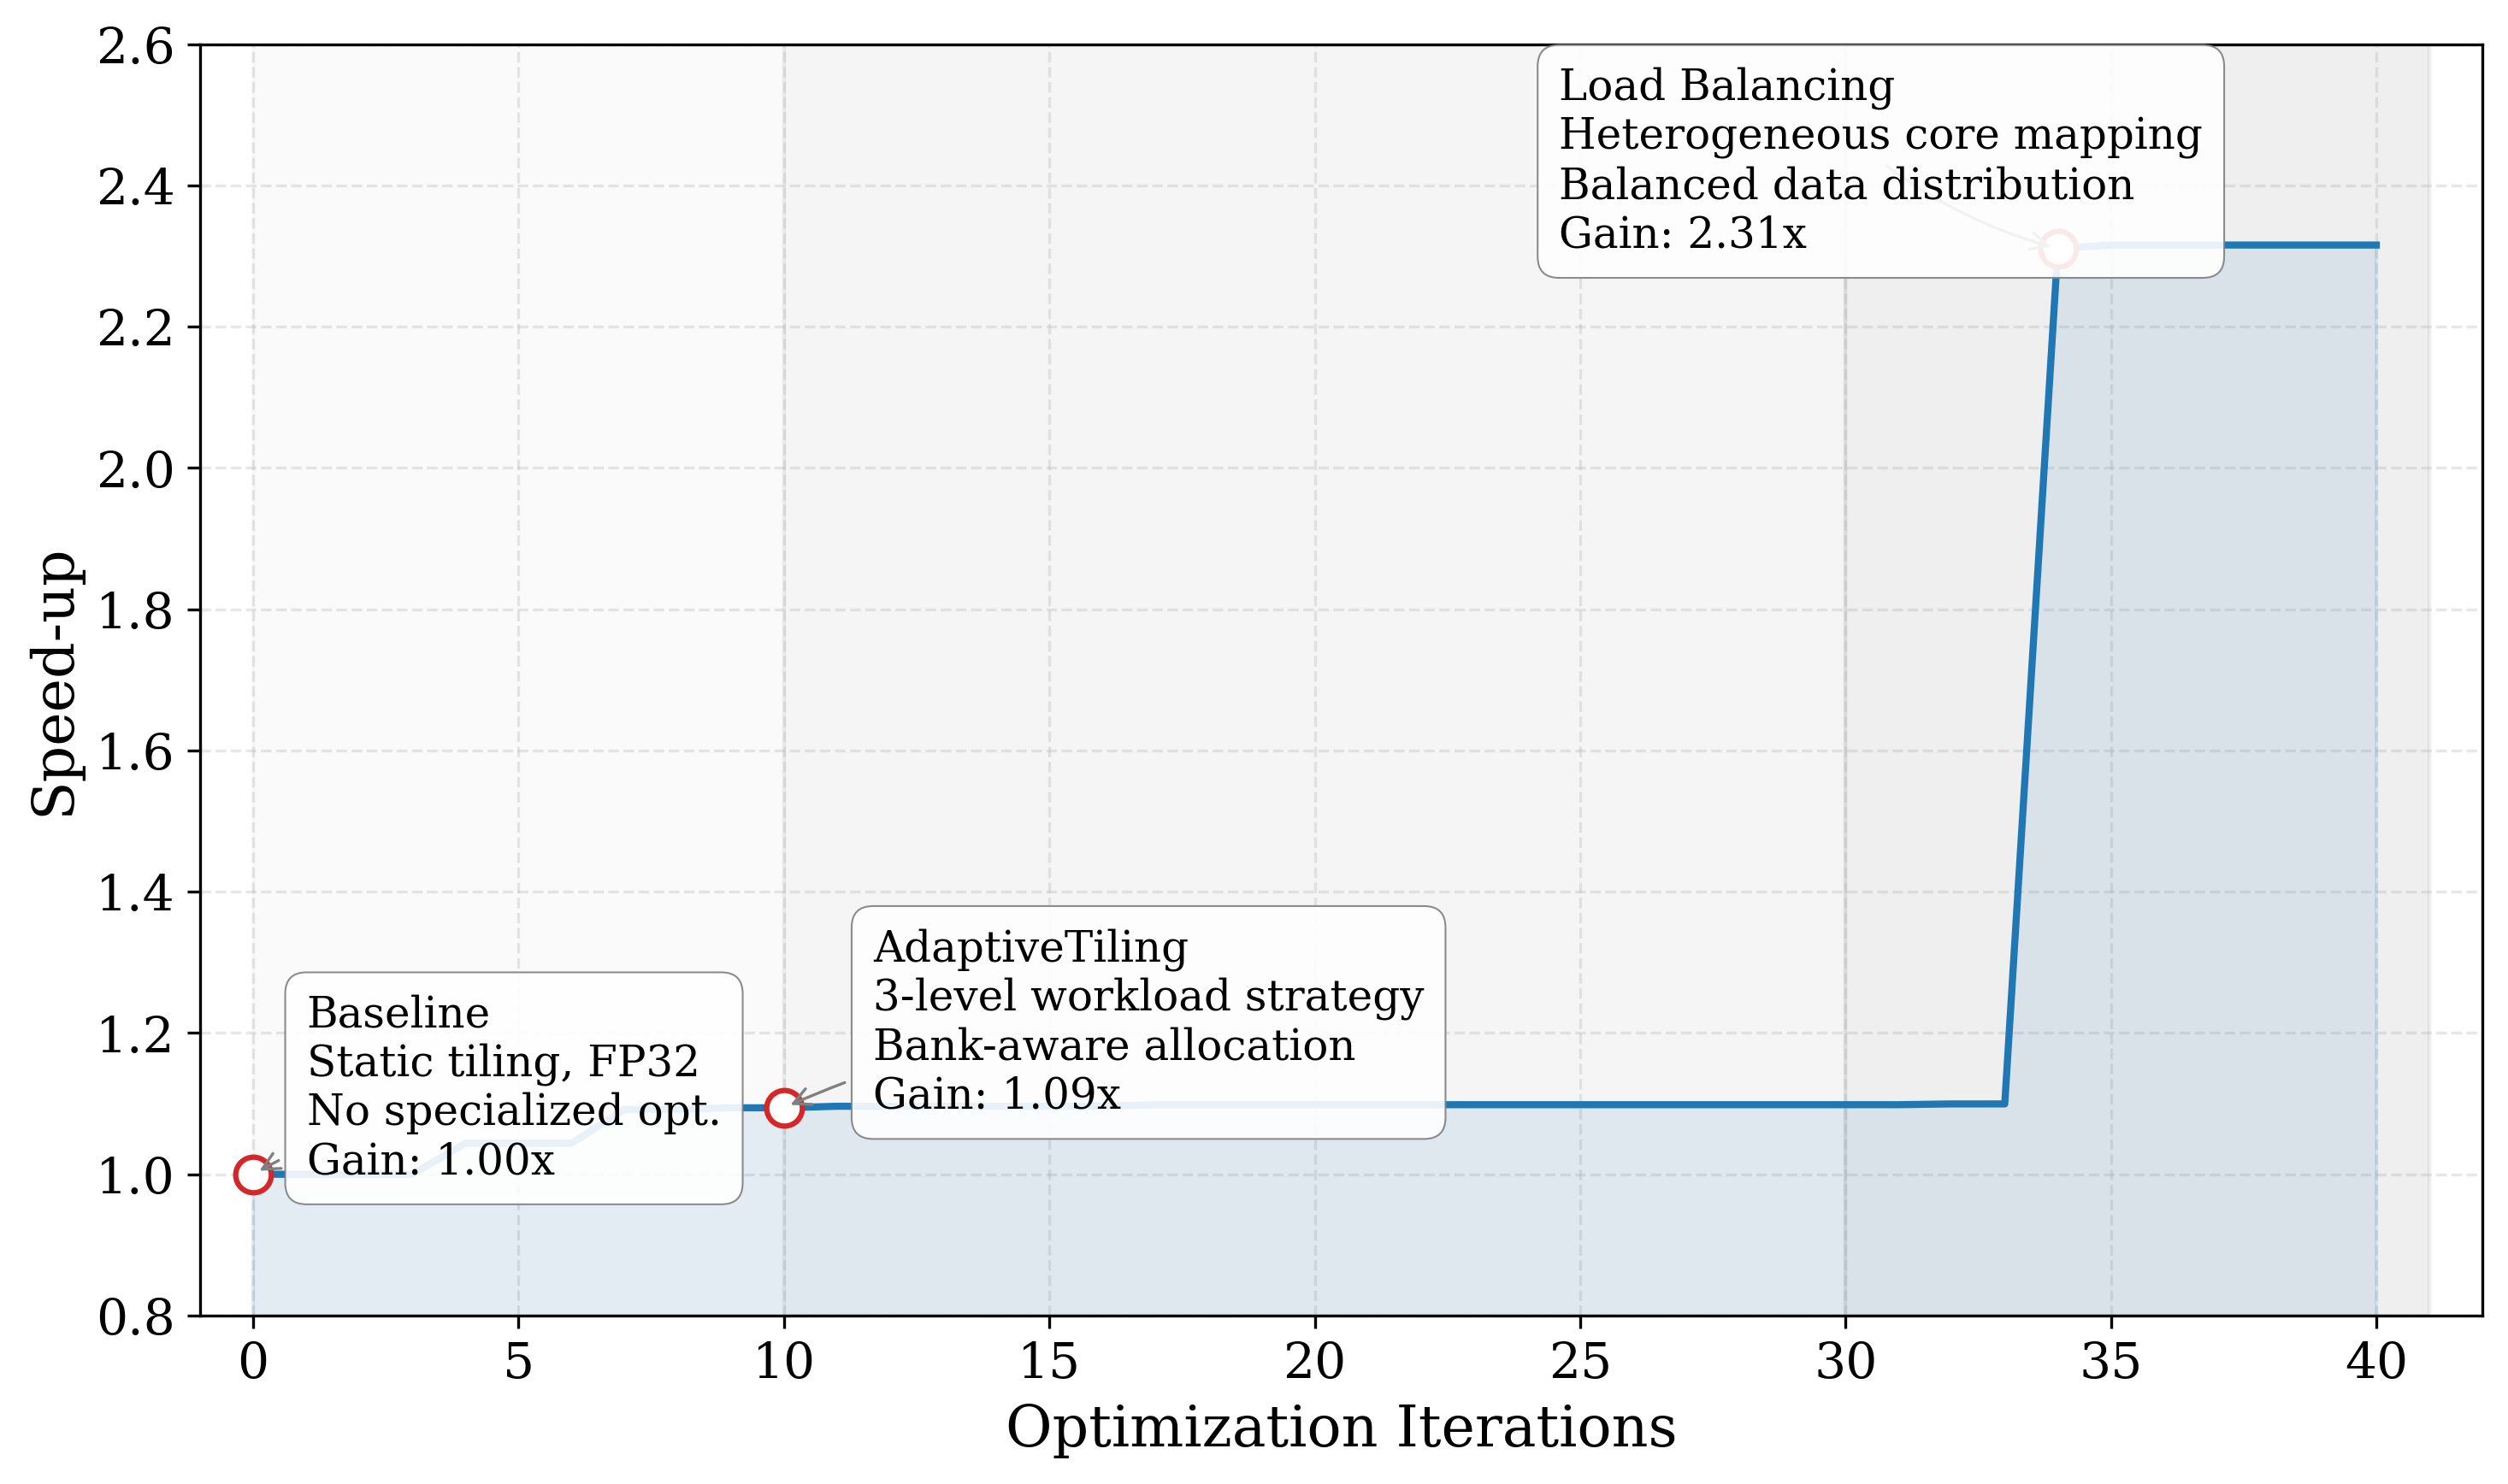
\includegraphics[width=0.45\textwidth]{fig/single_ops_curve.png}
%   \caption{Optimization trajectory of the "foreach\_pow\_scalar \\  
%   \_and\_tensor" operator.}
%   \label{fig:single_op_curve}
% \end{figure}


Figure~\ref{fig:single_op_curve} shows the optimization trajectory of "foreach\_pow\_scalar\_and\_tensor", illustrating how AscendOptimizer mitigates domain experience scarcity via an alternating two-stage loop.
The system switches every 10 iterations between Stage \Rmnum{1} (evolutionary tiling/execution tuning) and Stage \Rmnum{2} (experience-bank-driven semantic kernel rewriting).

On this operator, Stage \Rmnum{1} quickly delivers up to a $\num{1.09}\times$ speedup but then plateaus, indicating that further gains are bounded by the original kernel structure.In Stage \Rmnum{2}, the system diagnoses bottlenecks, retrieves relevant patterns, and applies semantic rewrites (e.g., pipelining/synchronization and mapping changes). \Cref{fig:code_diff} illustrates a representative rewrite: we replace the remainder-based per-core quota assignment with block-level load balancing and a nested scan across tensors, which reduces tail imbalance and improves core utilization. Correspondingly, a major jump at iteration 33 (within a Stage \Rmnum{2} period) introduces a more effective heterogeneous core mapping and reaches $\num{2.31}\times$.
Overall, Stage \Rmnum{1} exploits the remaining tuning headroom, while Stage \Rmnum{2} injects reusable experience to break structural bottlenecks.
\begin{figure}[H]
\centering
{\lstset{basicstyle=\ttfamily\scriptsize,
  columns=fullflexible,
  keepspaces=true,
  showstringspaces=false,
  frame=none,
  breaklines=true,
  breakatwhitespace=true,
  escapeinside={(*@}{@*)}}
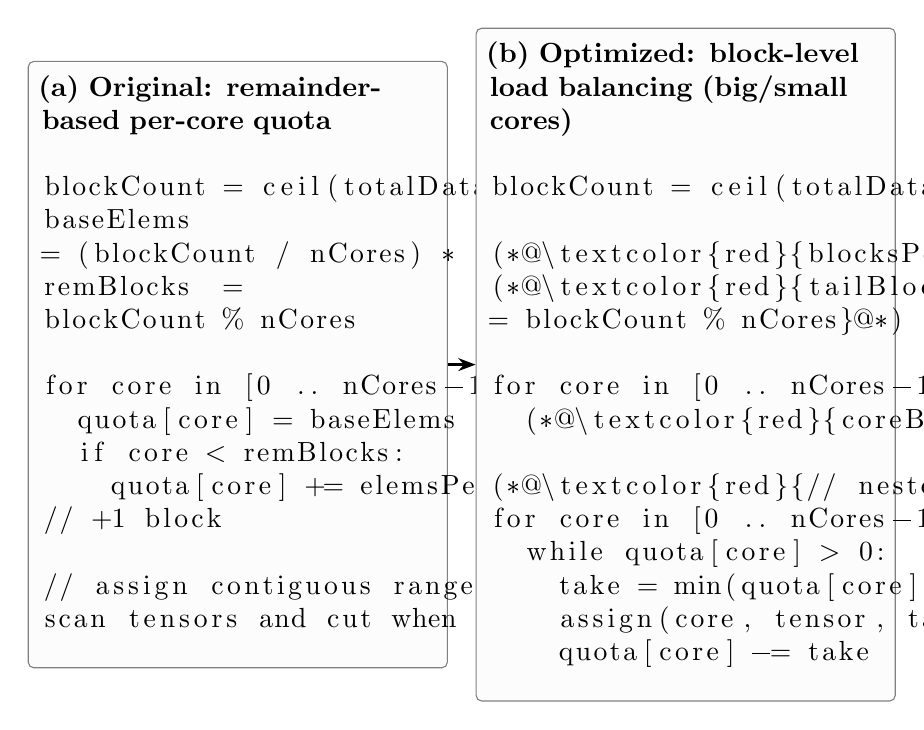
\begin{tikzpicture}[
  box/.style={
    draw=black!50,
    rounded corners=2pt,
    inner sep=5pt,
    align=left,
    text width=0.41\linewidth,
    fill=black!1
  },
  >={Stealth[length=2.2mm]}
]

% ---------- (a) Original ----------
\node[box] (A) {
\textbf{(a) Original: remainder-based per-core quota}\par\medskip
\begin{lstlisting}
blockCount = ceil(totalData / elemsPerBlock)
baseElems  = (blockCount / nCores) * elemsPerBlock
remBlocks  =  blockCount % nCores

for core in [0 .. nCores-1]:
  quota[core] = baseElems
  if core < remBlocks:
    quota[core] += elemsPerBlock   // +1 block

// assign contiguous ranges to each core
scan tensors and cut when used == quota[core]
\end{lstlisting}
};

% ---------- (b) Optimized ----------
\node[box, right=10pt of A] (B) {
\textbf{(b) Optimized: block-level load balancing (big/small cores)}\par\medskip
\begin{lstlisting}
blockCount = ceil(totalData / elemsPerBlock)

(*@\textcolor{red}{blocksPerCore = blockCount / nCores}@*)
(*@\textcolor{red}{tailBlocks    = blockCount % nCores}@*)

for core in [0 .. nCores-1]:
  (*@\textcolor{red}{coreBlocks = blocksPerCore + (core < tailBlocks)}@*)quota[core] = (*@\textcolor{red}{coreBlocks}@*) * elemsPerBlock

(*@\textcolor{red}{// nested scan: fill each core's quota across tensors}@*)
for core in [0 .. nCores-1]:
  while quota[core] > 0:
    take = min(quota[core], remaining(tensor))
    assign(core, tensor, take)
    quota[core] -= take
\end{lstlisting}
};

% ---------- Arrow ----------
\draw[->, thick] (A.east) -- (B.west);

\end{tikzpicture}
}

\captionsetup{justification=raggedright,singlelinecheck=false}
\caption{Illustration of a key scheduling rewrite in \texttt{foreach\_\allowbreak pow\_\allowbreak scalar\_\allowbreak and\_\allowbreak tensor}: (a) the original remainder-based per-core quota assignment; (b) the optimized block-level load balancing with a nested scan across tensors (changes highlighted in red).}
\label{fig:code_diff}
\end{figure}
% On this operator, Stage \Rmnum{1} quickly delivers up to a $\num{1.09}\times$ speedup but then plateaus, indicating that further gains are bounded by the original kernel structure.
%
%
% ====== Required packages ======
% \usepackage{tikz}
% \usepackage{xcolor}
% \usepackage{listings}
% \usetikzlibrary{arrows.meta,positioning}
%
% \lstset{
%   basicstyle=\ttfamily\small,
%   columns=fullflexible,
%   keepspaces=true,
%   showstringspaces=false,
%   frame=none,
%   breaklines=true,
%   breakatwhitespace=true,
%   escapeinside={(*@}{@*)}
% }
%
% \begin{figure*}[htbp]
% \centering
% \begin{tikzpicture}[
%   box/.style={
%     draw=black!50,
%     rounded corners=1.5pt,
%     inner sep=6pt,
%     align=left,
%     text width=0.46\linewidth
%   },
%   >={Stealth[length=2.2mm]}
% ]
%
% % ---------- (a) Original ----------
% \node[box] (A) {
% \textbf{(a) Original: remainder-based per-core quota}\par\medskip
% \begin{lstlisting}
% blockCount = ceil(totalData / elemsPerBlock)
% baseElems  = (blockCount / nCores) * elemsPerBlock
% remBlocks  =  blockCount % nCores
%
% for core in [0 .. nCores-1]:
%   quota[core] = baseElems
%   if core < remBlocks:
%     quota[core] += elemsPerBlock   // +1 block
%
% // assign contiguous ranges to each core
% scan tensors and cut when used == quota[core]
% \end{lstlisting}
% };
%
% % ---------- (b) Optimized ----------
% \node[box, right=12pt of A] (B) {
% \textbf{(b) Optimized: block-level load balancing (big/small cores)}\par\medskip
% \begin{lstlisting}
% blockCount = ceil(totalData / elemsPerBlock)
%
% (*@\textcolor{red}{blocksPerCore = blockCount / nCores}@*)
% (*@\textcolor{red}{tailBlocks    = blockCount % nCores}@*)
%
% for core in [0 .. nCores-1]:
%   (*@\textcolor{red}{coreBlocks = blocksPerCore + (core < tailBlocks)}@*)
%   quota[core] = (*@\textcolor{red}{coreBlocks}@*) * elemsPerBlock
%
% (*@\textcolor{red}{// nested scan: fill each core's quota across tensors}@*)
% for core in [0 .. nCores-1]:
%   while quota[core] > 0:
%     take = min(quota[core], remaining(tensor))
%     assign(core, tensor, take)
%     quota[core] -= take
% \end{lstlisting}
% };
%
% % ---------- Arrow ----------
% \draw[->, thick] (A.east) -- (B.west);
%
% \end{tikzpicture}
%
% \captionsetup{justification=raggedright,singlelinecheck=false}
% % \caption{Illustration of a key scheduling rewrite in \texttt{foreach\_\allowbreak pow\_\allowbreak scalar\_\allowbreak and\_\allowbreak tensor}: (a) the original remainder-based per-core quota assignment; (b) the optimized block-level load balancing with a nested scan across tensors (changes highlighted in red).}
% \label{fig:code_diff}
% \end{figure*}
%
%
% \begin{figure}[htbp]
%   \centering
%   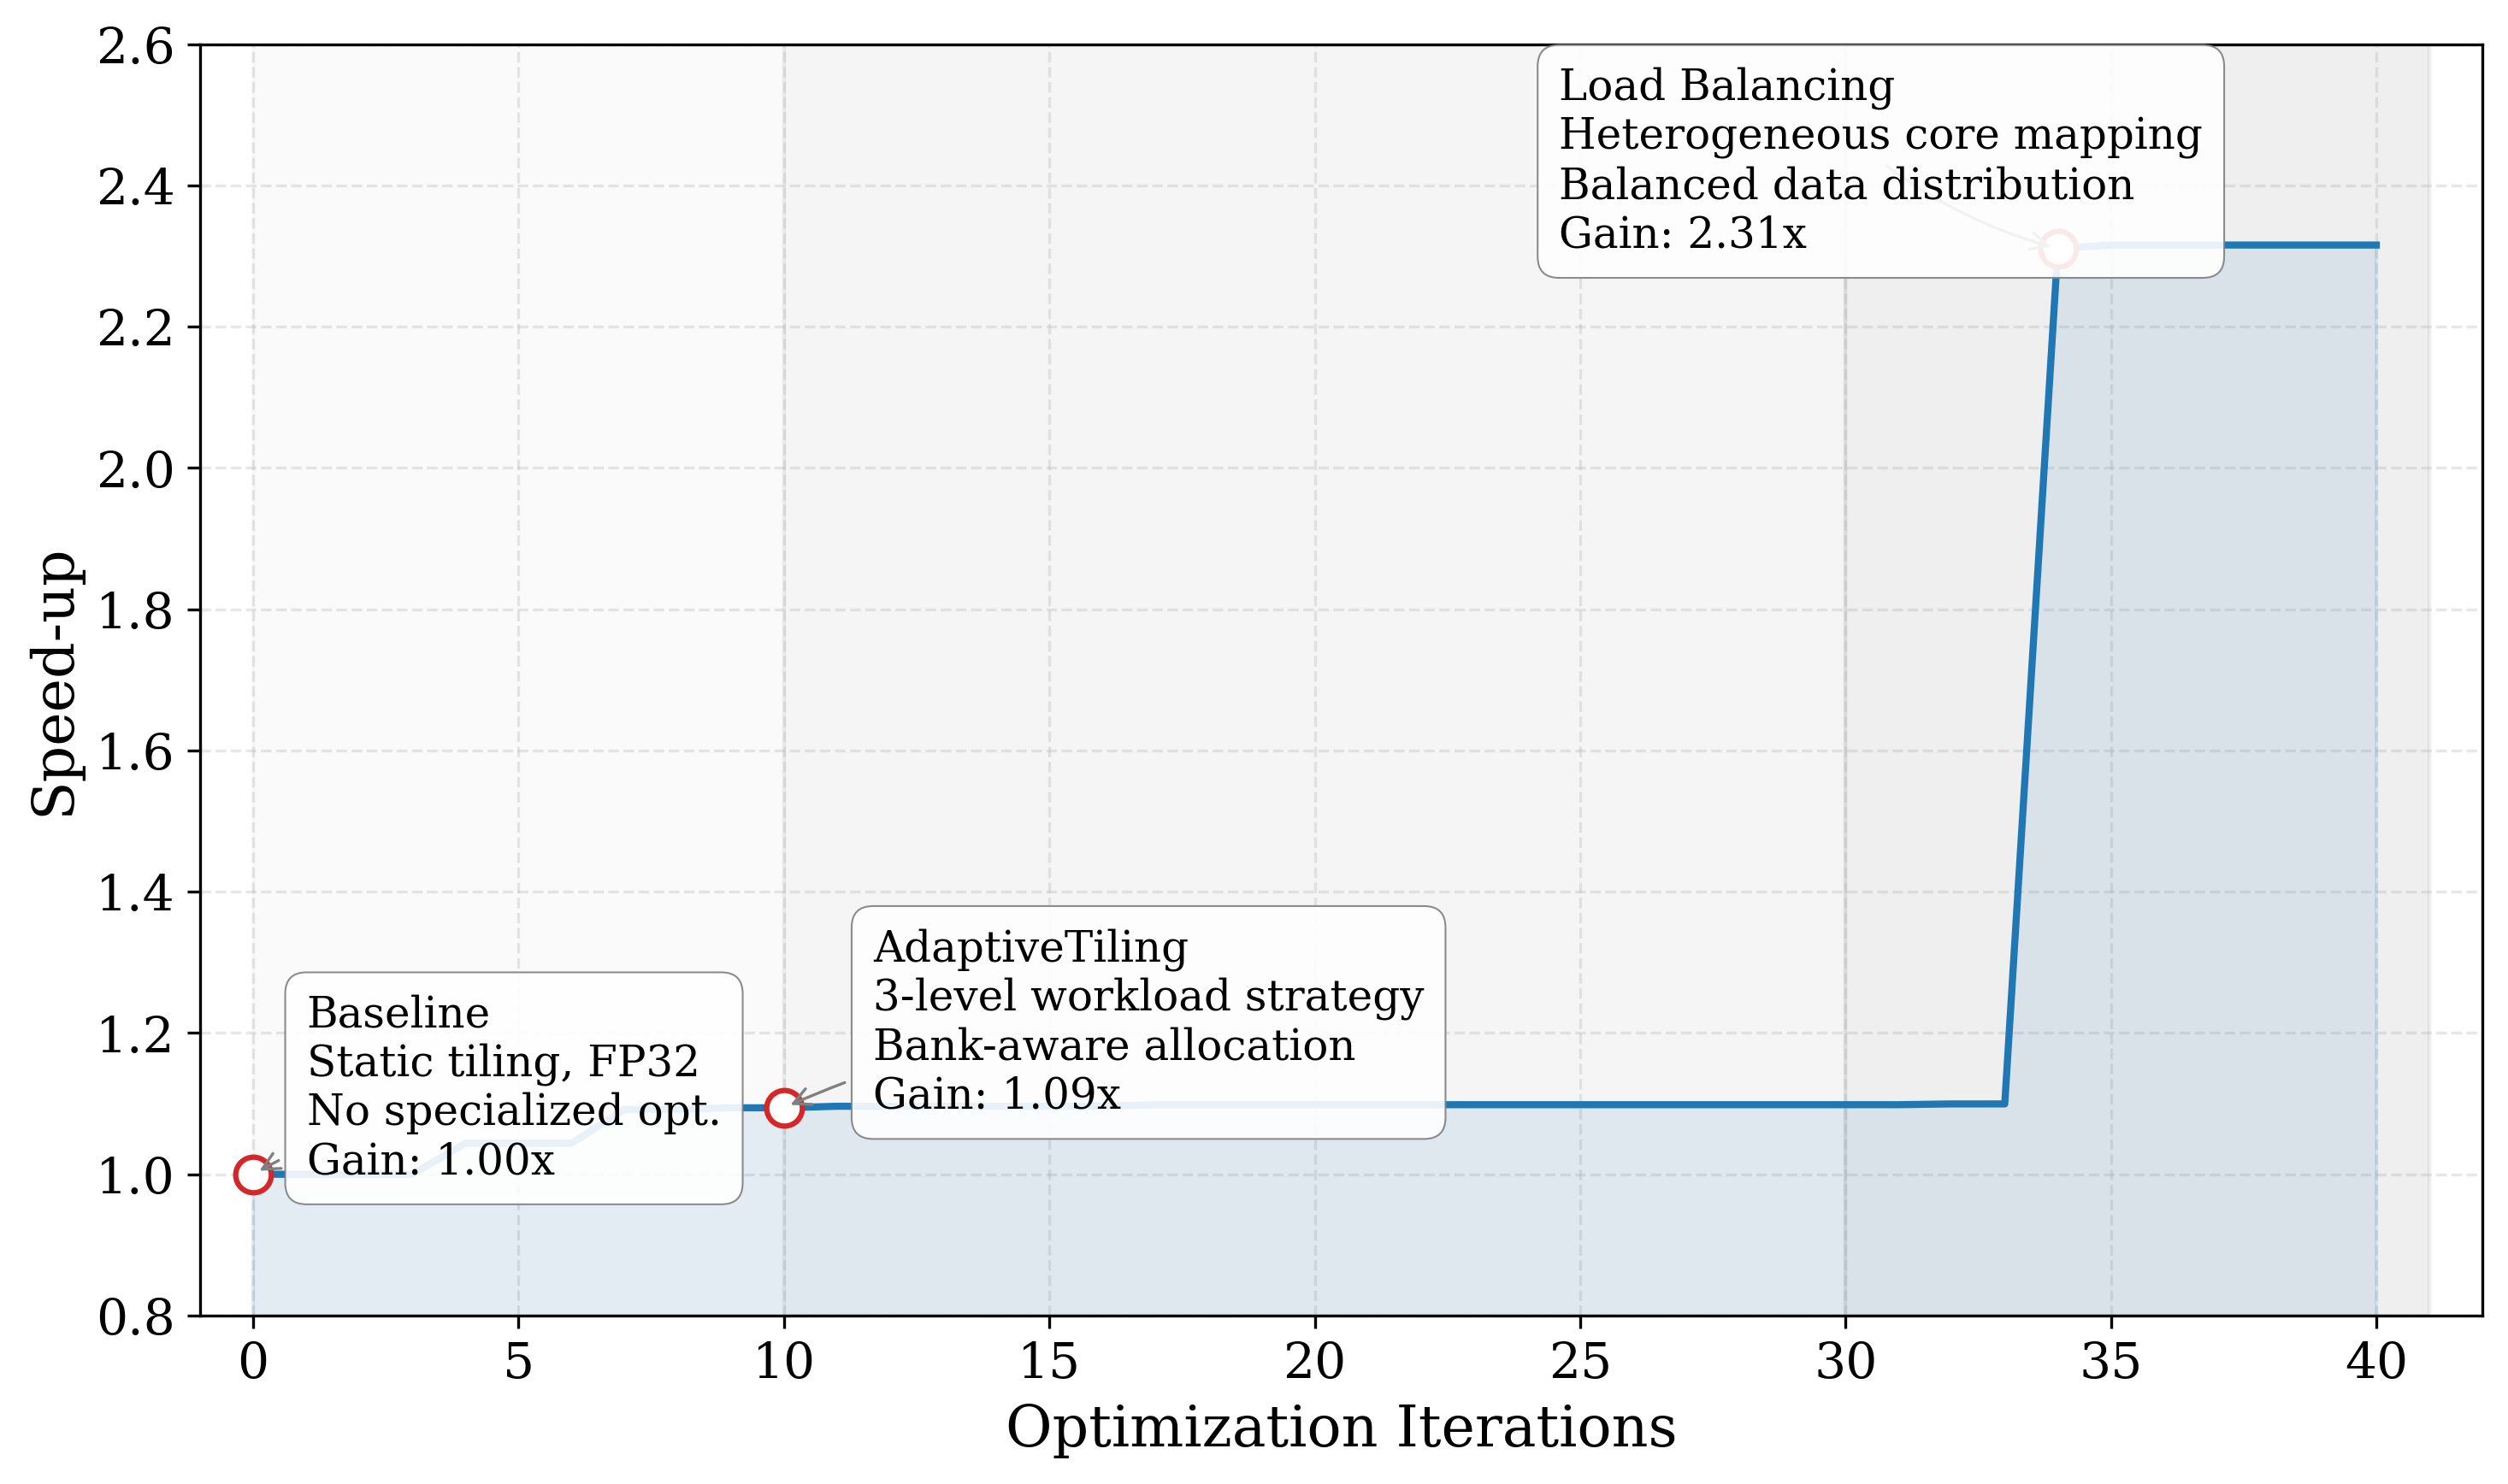
\includegraphics[width=0.45\textwidth]{fig/single_ops_curve.png}
%   \caption{Optimization trajectory of the "foreach\_pow\_scalar \\  
%   \_and\_tensor" operator.}
%   \label{fig:single_op_curve}
% \end{figure}
% In Stage \Rmnum{2}, the system diagnoses bottlenecks, retrieves relevant patterns, and applies semantic rewrites (e.g., pipelining/synchronization and mapping changes). \Cref{fig:code_diff} illustrates a representative rewrite: we replace the remainder-based per-core quota assignment with block-level load balancing and a nested scan across tensors, which reduces tail imbalance and improves core utilization. Correspondingly, a major jump at iteration 33 (within a Stage \Rmnum{2} period) introduces a more effective heterogeneous core mapping and reaches $\num{2.31}\times$.
% Overall, Stage \Rmnum{1} exploits the remaining tuning headroom, while Stage \Rmnum{2} injects reusable experience to break structural bottlenecks.
% Figure~\ref{fig:single_op_curve} illustrates the optimization trajectory of the \texttt{foreach\_pow} operator, serving as a representative case to demonstrate how the proposed framework addresses domain experience scarcity through two distinct stages. Notably, this trajectory closely mirrors the optimization process typically followed by experienced human developers.

% As shown in Figure~\ref{fig:single_op_curve}, the optimization of \texttt{foreach\_pow} exhibits a typical \emph{two-stage alternating} trajectory: the system switches every \textbf{10 iterations} between Stage \Rmnum{1} (tiling/execution configuration exploration) and Stage \Rmnum{2} (experience-bank-driven semantic kernel rewriting). This case indicates that, for \texttt{foreach\_pow}, parameter search delivers early gains but soon enters a clear plateau; once experience-bank-based retrieval and semantic rewriting are introduced, the curve shows a structural jump, suggesting that experience injection helps overcome bottlenecks that are difficult to surpass by tuning alone.

% \paragraph{Stage I: Rapid gains and periodic saturation of parameter exploration (executed every 10 iterations).}
% During each Stage \Rmnum{1} period, AscendOptimizer performs an evolutionary search over tiling decisions and execution parameters, and leverages real NPU performance feedback to obtain up to a $1.09\times$ speedup in the tiling search phase. As multiple Stage \Rmnum{1} periods proceed, the curve gradually enters a plateau: further expanding the parameter exploration yields diminishing or no improvements, indicating that the bottleneck has shifted from \emph{tunable parameters} to \emph{structural limitations} of the existing kernel logic and mapping, where tuning alone becomes insufficient.

% \paragraph{Stage II: experience-driven semantic rewriting and performance leap (executed every 10 iterations).}
% During each Stage \Rmnum{2} period, the system first diagnoses performance bottlenecks in the current kernel, then retrieves similar optimization patterns from the experience bank, and finally applies them via a rewriting module as semantic-level code transformations (e.g., improved pipelining/synchronization strategies and execution mapping). The pronounced jump at iteration 33 occurs within the corresponding Stage \Rmnum{2} period: the retrieved pattern matches the operator’s bottleneck well, enabling a structural rewrite that successfully introduces a more effective heterogeneous core mapping strategy, pushing the speedup to $2.31\times$. In essence, Stage \Rmnum{2} provides the capability to reorganize the AscendC computation pipeline, whose benefits are typically unattainable by further extending Stage \Rmnum{1} parameter search.

% \paragraph{Takeaway.}
% This case highlights the complementarity of the alternating two-stage design. Stage \Rmnum{1} efficiently exploits the available tuning space under implicit hardware constraints and reliably identifies the boundary of tuning gains, whereas Stage \Rmnum{2} periodically injects reusable optimization experience to enable larger-granularity semantic rewrites of the kernel. Together, they form an “exploration--experience-driven breakthrough” loop, allowing AscendOptimizer to achieve sustained and transferable improvements even in the absence of hand-crafted expert rules and supervised optimization data.

\FloatBarrier
\section{Conclusion}
\label{sec:conclusion}
This work targets the challenge of automatic generation and optimization of AscendC operators on Ascend NPUs under severe scarcity of expert knowledge and training data. We propose AscendOptimizer, a two-stage self-bootstrapped framework that enables end-to-end optimization without hand-crafted rules or additional model training. We cast optimization as a joint search over host-side tiling configurations and AI Core kernel logic, and exploit their distinct search-space characteristics via a divide-and-conquer design: Stage \Rmnum{1} leverages hardware-in-the-loop compilation and on-device performance feedback to synthesize high-performance feasible tiling configurations through evolutionary search; Stage \Rmnum{2} constructs a retrievable, structured optimization memory via rewind and applies retrieval-augmented semantic kernel rewriting to overcome structural bottlenecks beyond parameter tuning. Experimental results demonstrate that the proposed framework yields consistent performance improvements and outperforms strong baselines. Future work will improve robustness to dynamic shapes and cross-stack variability, reduce hardware-in-the-loop overhead, and strengthen noise tolerance and correctness assurance.


% \clearpage
% \newpage

% TODO:limitation,没有适配动态shape
% In the unusual situation where you want a paper to appear in the
% references without citing it in the main text, use \nocite
\nocite{langley00}

\bibliography{example_paper}
\bibliographystyle{plain}

%%%%%%%%%%%%%%%%%%%%%%%%%%%%%%%%%%%%%%%%%%%%%%%%%%%%%%%%%%%%%%%%%%%%%%%%%%%%%%%
%%%%%%%%%%%%%%%%%%%%%%%%%%%%%%%%%%%%%%%%%%%%%%%%%%%%%%%%%%%%%%%%%%%%%%%%%%%%%%%
% APPENDIX
%%%%%%%%%%%%%%%%%%%%%%%%%%%%%%%%%%%%%%%%%%%%%%%%%%%%%%%%%%%%%%%%%%%%%%%%%%%%%%%
%%%%%%%%%%%%%%%%%%%%%%%%%%%%%%%%%%%%%%%%%%%%%%%%%%%%%%%%%%%%%%%%%%%%%%%%%%%%%%%
\newpage
\appendix
\onecolumn

\section{Additional Experimental Details}
\label{app:exp_details}

% \paragraph{Benchmark construction and filtering.}
% We start from the \texttt{cann-ops} AscendC operator repository and use the provided implementations as our baseline.
% During preparation, we (i) verify compilability, (ii) check numerical correctness against a CPU reference, and (iii) remove operators that fail compilation/execution or violate correctness.

% \paragraph{Input-shape adjustment (noise reduction).}
% Because hardware-level timing can be noisy for small workloads, we moderately increase the input shapes for a subset of operators to improve runtime stability and make performance differences more observable. To minimize threats to validity, we follow three safeguards: (i) we only apply shape changes that preserve operator semantics (e.g., scaling batch/sequence/spatial dimensions without changing the computation type); (ii) for each affected operator, we evaluate \emph{both} the baseline and all optimized variants under the \emph{same} adjusted shape (so reported speedups remain comparable); and (iii) we keep the scaling factor small and report the original and adjusted shapes in this appendix.

\paragraph{Final benchmark size.}
After these checks and adjustments, we retain 127 operators for all reported experiments.
% 更紧凑的 LaTeX 表格：同一模块的算子合并到一行里
% 如需自动换行可用 p{<width>}，这里用 p{0.78\linewidth} 让第二列自动折行
% \usepackage{array}

\begin{tabular}{@{}l p{0.78\linewidth}@{}}
\hline
\textbf{Category} & \textbf{Operator} \\
\hline
level1 (43) &  add\_custom, addcdiv, addcmul, angle\_v2, arange, cast, ccopy, clip\_by\_value\_v2, complex\_mat\_dot, cos, equal, eye, eye\_fp64, fill, gcd, greater\_equal, heaviside, icamax, icamin, is\_inf, isamax, isamin, lerp, less, less\_equal, lin\_space, logical\_not, logical\_or, muls, neg, non\_finite\_check, reciprocal, reshape, rsqrt, sasum, scasum, scnrm2, scopy, snrm2, sqrt, sscal, strideslice\_neg\_concat\_v2, trunc \\
level2 (77) & ge\_glu\_grad\_v2, ge\_glu\_v2, ge\_glu\_v3, gelu\_quant, swi\_glu, swi\_glu\_grad, circular\_pad, pad\_v3\_grad\_replication, reflection\_pad3d\_grad, strided\_slice\_assign\_v2, foreach\_acos, foreach\_add\_list, foreach\_add\_scalar, foreach\_add\_scalar\_list, foreach\_addcdiv\_scalar, foreach\_addcmul\_scalar, foreach\_addcmul\_scalar\_list, foreach\_asin, foreach\_copy, foreach\_cos, foreach\_div\_list, foreach\_div\_scalar, foreach\_erf, foreach\_erfc, foreach\_exp, foreach\_expm1, foreach\_lerp\_scalar, foreach\_log2, foreach\_maximum\_scalar, foreach\_minimum\_scalar, foreach\_mul\_list, foreach\_mul\_scalar, foreach\_neg, foreach\_non\_finite\_check\_and\_unscale, foreach\_pow\_scalar, foreach\_pow\_scalar\_and\_tensor, foreach\_reciprocal, foreach\_round\_off\_number, foreach\_sigmoid, foreach\_sign, foreach\_sinh, foreach\_sqrt, foreach\_sub\_scalar, foreach\_tan, foreach\_tanh, foreach\_zero\_inplace, motion\_compensation, upsample\_bicubic2d\_aa\_grad, upsample\_bilinear2d\_aa, upsample\_bilinear2d\_aa\_backward, upsample\_bilinear2d\_grad, upsample\_nearest\_exact3d, upsample\_trilinear3d\_backward, feeds\_repeat, cross\_entropy\_loss, add\_sigmoid\_mul\_reduce\_sum\_d, cross, expand\_v2, fast\_gelu\_grad, gelu, gelu\_grad, inplace\_fused\_matmul\_softmax\_grad, kl\_div\_target\_backward, mul\_sigmoid, swish, tril, triu, add\_layer\_norm, add\_layer\_norm\_grad, add\_rms\_norm\_dynamic\_quant, add\_rms\_norm\_quant, deep\_norm, group\_norm\_swish, rms\_norm, rms\_norm\_grad, adaptive\_avg\_pool3d\_grad, avg\_pool3\_d \\
level3 (7) & bev\_pool, flash\_attention\_score\_with\_large\_head\_dim, matmul\_all\_reduce, matmul\_api\_constant, matmul\_leakyrelu, matmul\_reduce\_scatter, complex\_mat\_mul \\
\hline
\end{tabular}

\section{Method Details and Experience Bank Analysis}
\label{app:method_experience}
This section provides additional analyses of the optimization experience bank and detailed method snippets.

% A consistent style for appendix code blocks.
% If you want syntax highlighting, change language=C++ to the actual language.
\lstdefinestyle{appendixcode}{
  basicstyle=\ttfamily\footnotesize,
  columns=fullflexible,
  keepspaces=true,
  showstringspaces=false,
  breaklines=true,
  breakatwhitespace=true,
  frame=single,
  framerule=0.3pt,
  rulecolor=\color{black!30},
  xleftmargin=0.5em,
  xrightmargin=0.5em,
  aboveskip=0.6em,
  belowskip=0.6em,
  numbers=left,
  numberstyle=\tiny\color{black!50},
  numbersep=6pt,
  tabsize=2,
  captionpos=b,
  language=C++
}

% \begin{figure}[t]
% \centering
% \begin{minipage}{\linewidth}
% \lstset{style=appendixcode}
% \begin{lstlisting}
% // TODO: paste code snippet here.
% // Suggested: include a short comment describing what this code demonstrates.
% \end{lstlisting}
% \end{minipage}
% \caption{Example code listing (replace with the actual kernel/tiling code).}
% \label{fig:appendix_code_placeholder}
% \end{figure}

\subsection{Experience Bank Analysis}
\paragraph{Methodological Comparison of Optimization Experience Sources.}
Table~\ref{tab:experience_comparison} compares the official Ascend C best practices with the optimization experience bank constructed in this work from a experience representation perspective.



The comparison shows that while official documentation provides stable and interpretable optimization rules for human developers, the proposed experience bank captures optimization experience in a machine-consumable form, enabling direct integration with automated code generation and optimization pipelines.

\paragraph{Validation and extension beyond documented best practices.}
Based on the observed semantic structure, Table~\ref{tab:validation_extension} summarizes how the automatically constructed experience bank relates to the official Ascend C best practices at the optimization semantics level.
This case study demonstrates that the proposed optimization experience bank not only reproduces and refines optimization principles explicitly documented in official Ascend C best practices, but also systematically uncovers implicit optimization behaviors that are not formally documented. By organizing such experience in a retrieval-augmented and machine-consumable form, the experience bank provides effective support for automated operator-level code optimization.

% \begin{figure*}[htbp]
% \centering
% 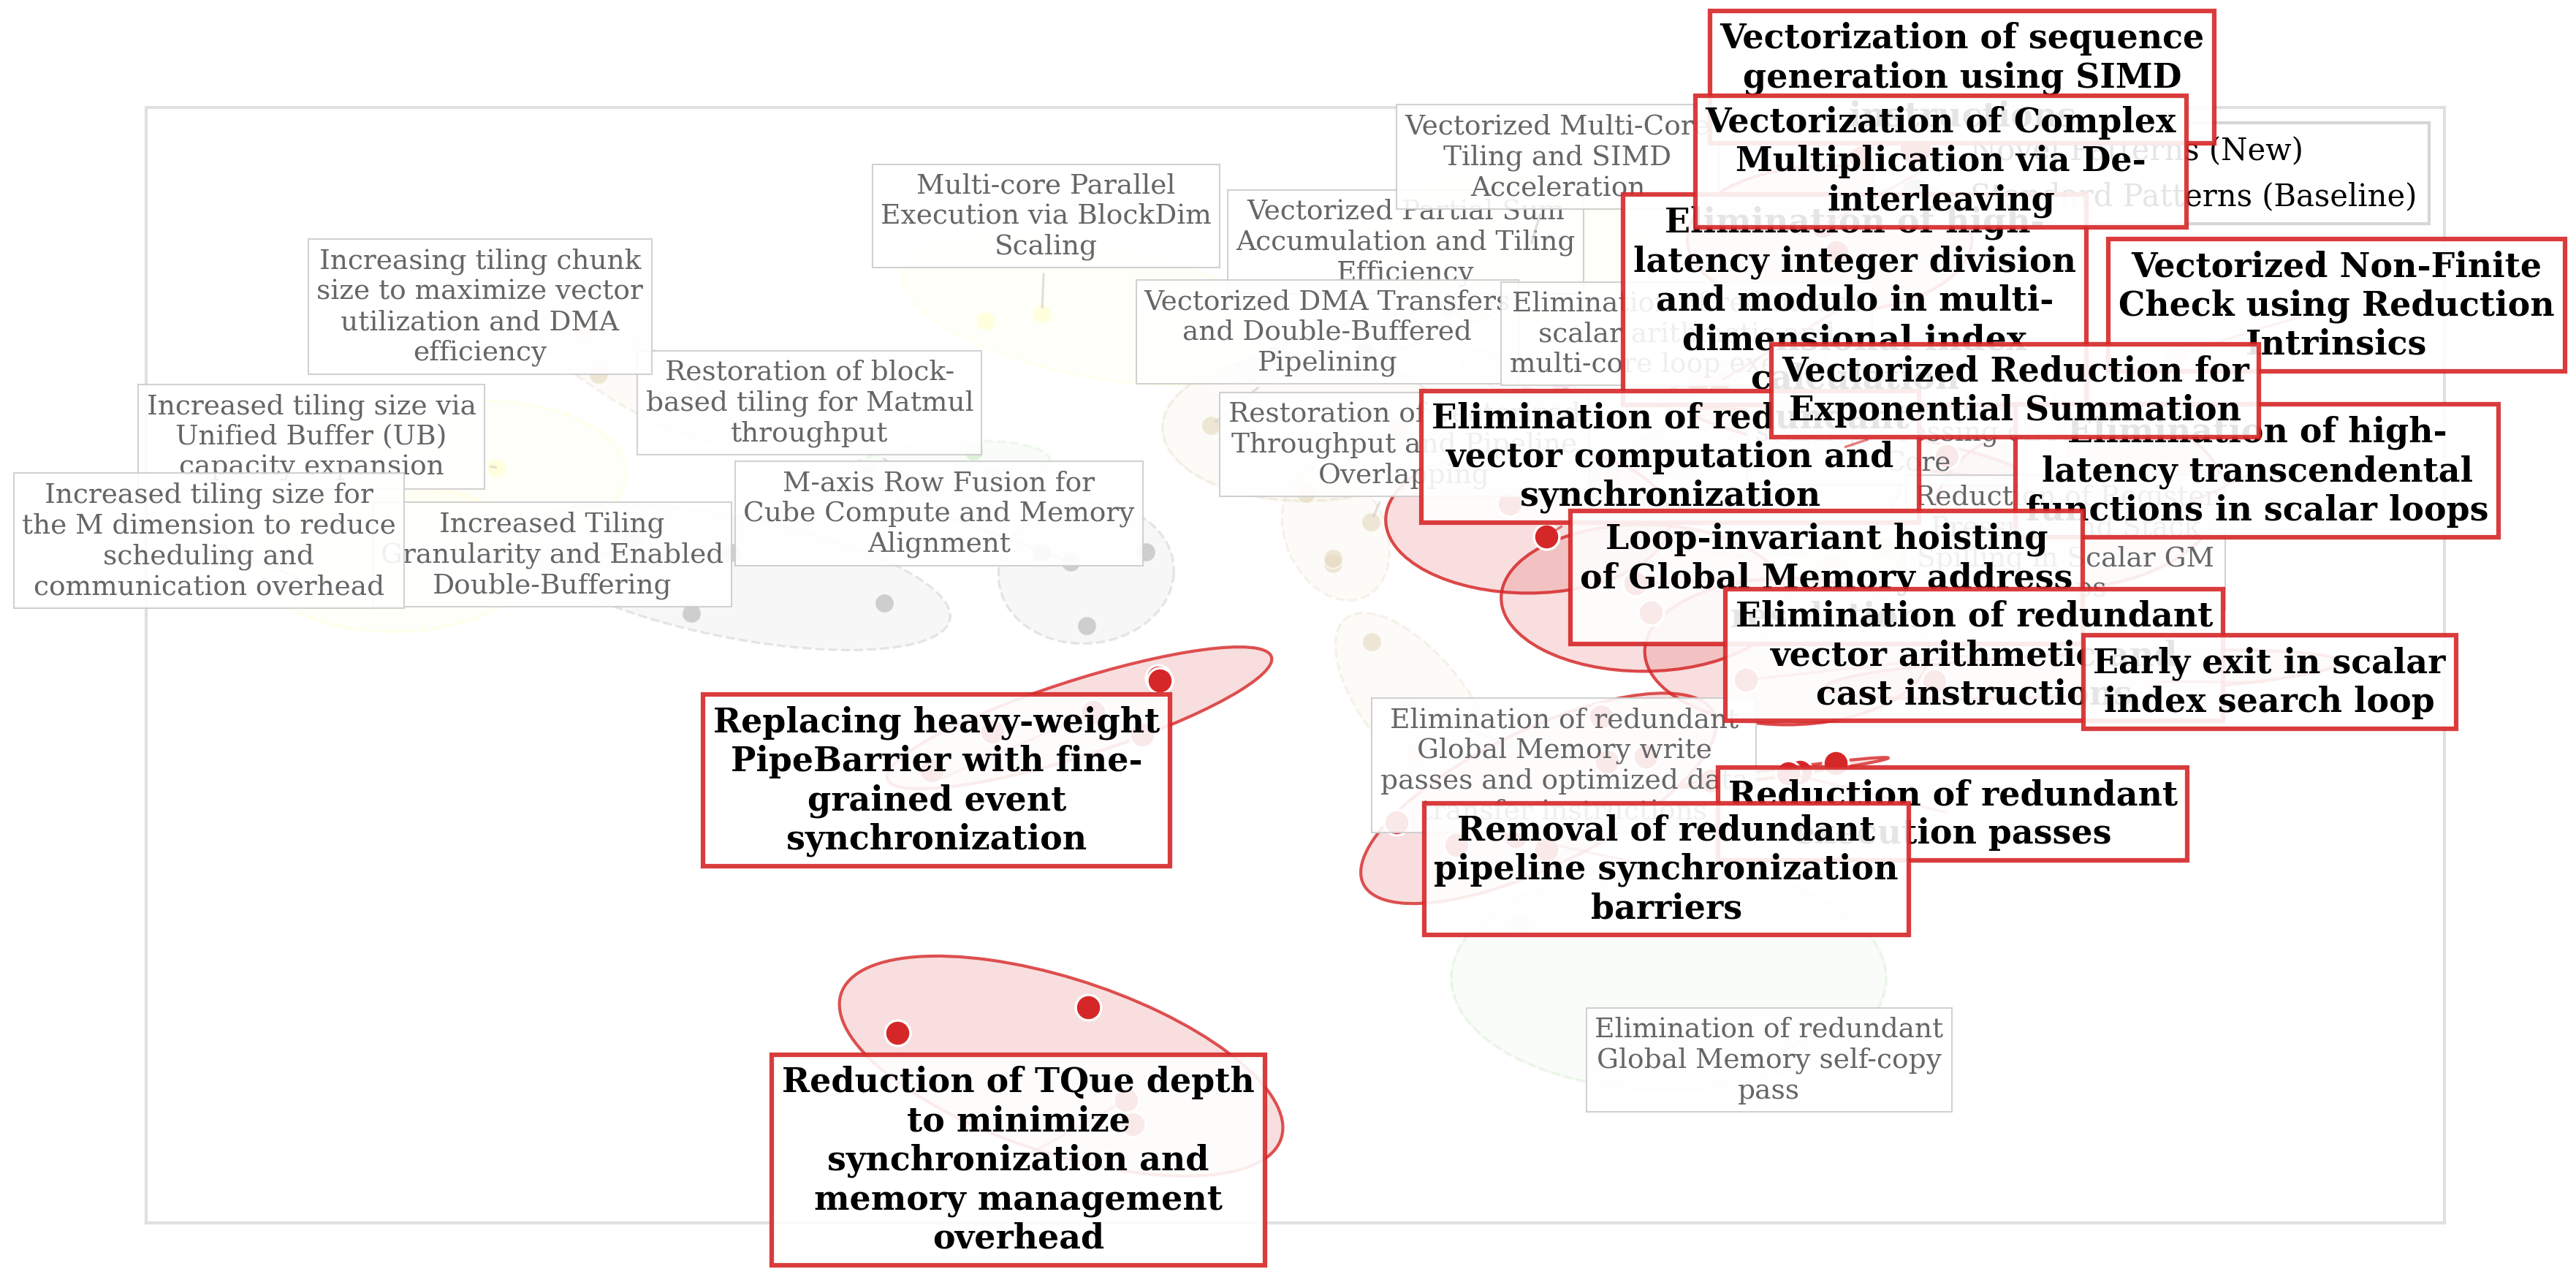
\includegraphics[width=0.65\textwidth]{fig/cluster_scatter_llm.png}
% \caption{Semantic landscape of optimization strategies via embedding clustering.
% Each optimization record (Title \& Description) is embedded using an embedding model, projected to 2D for visualization with PCA, and clustered with K-Means.
% Grey/light regions denote clusters aligned with categories described in the official documentation, while red regions denote clusters that do not directly correspond to the documentation’s explicit taxonomy.}
% \label{fig:semantic_landscape}
% \end{figure*}


\begin{table*}[htb!]
\centering
\caption{Comparison between official Ascend C best practices and the automatically constructed optimization experience bank}
\label{tab:experience_comparison}
\resizebox{\linewidth}{!}{%
\begin{tabular}{p{3.2cm} p{5.2cm} p{5.6cm}}
\toprule

\textbf{Dimension} & \textbf{Official Ascend C Best Practices} & \textbf{Automatically Constructed Experience Bank} \\
\midrule
Experience acquisition
& Manual summarization of long-term expert engineering experience
& Automatic mining via self-supervised rewind on benchmarks \\

Experience form
& Explicit rules and guidelines (rule-based)
& Implicit optimization patterns distilled from code differences \\

Granularity
& Coarse-grained, principle-level (e.g., ``increase tiling'', ``reduce GM access'')
& Fine-grained, statement-, instruction-, and pipeline-level rewrite patterns \\

Coverage scope
& Common and generalizable optimization scenarios
& Long-tail operator shapes, non-typical control flow, and special data paths \\

Extensibility
& Static, requires continuous manual maintenance
& Automatically extensible with new benchmarks and operators \\

Support for automation
& No (primarily serves human developers)
& Yes (directly usable as RAG context for LLM-driven code rewriting) \\
\bottomrule
\end{tabular}%
}
\end{table*}


\begin{table*}[t]
\centering
\caption{Validation and extension of official Ascend C best practices by the optimization experience bank (selected examples)}
\label{tab:validation_extension}
\resizebox{\linewidth}{!}{%
\begin{tabular}{p{3.6cm} p{2.6cm} p{2.6cm} p{5.0cm} p{2.4cm}}
\toprule
\textbf{Optimization Category}
& \textbf{Covered in Docs}
& \textbf{Doc Granularity}
& \textbf{Observed Optimization Behavior (Representative Tags)}
& \textbf{Relation} \\
\midrule


Tiling size under UB capacity (arithmetic intensity)
& Yes
& Principle / case-level
& Increase tile size or restore block-tiling to raise compute intensity under UB constraints
& Validation + refinement \\

DMA efficiency and transfer consolidation
& Yes
& Mechanism-level
& Consolidate fragmented transfers and increase chunk size for better DMA startup amortization
& Validation + structuring \\

Double buffering and pipeline overlapping
& Yes
& Mechanism-level
& Enable/disable double buffering conditionally based on micro-tile size and sync cost
& Validation + conditionalization \\

Reduction intrinsics / vectorized reduction path
& Yes
& Guideline-level
& Choose vectorized reduction paths and hierarchical reduction for throughput scaling
& Validation + extension \\

Fine-grained synchronization and queue-depth tuning
& Partial
& Scattered / implicit
& Replace coarse barriers with finer events and tune internal queue depth to reduce management overhead
& Supplementing implicit experience \\

Scalar arithmetic and index computation simplification
& No
& --
& Remove high-latency div/mod and simplify multi-dimensional index computation in scalar loops
& Undocumented \\

Scalar-loop algorithmic shortcuts (early-exit / search pruning)
& No
& --
& Add early termination conditions to scalar search loops to cut worst-case latency
& Undocumented \\

Specialized SIMD algorithm paths beyond generic best practices
& No
& --
& Domain-specific SIMD implementations not described as a general best practice
& Undocumented \\

\bottomrule
\end{tabular}%
}
\end{table*}
% Prevent this table from floating past the following section.
\FloatBarrier
% \begin{figure*}[htbp]
% \centering
% 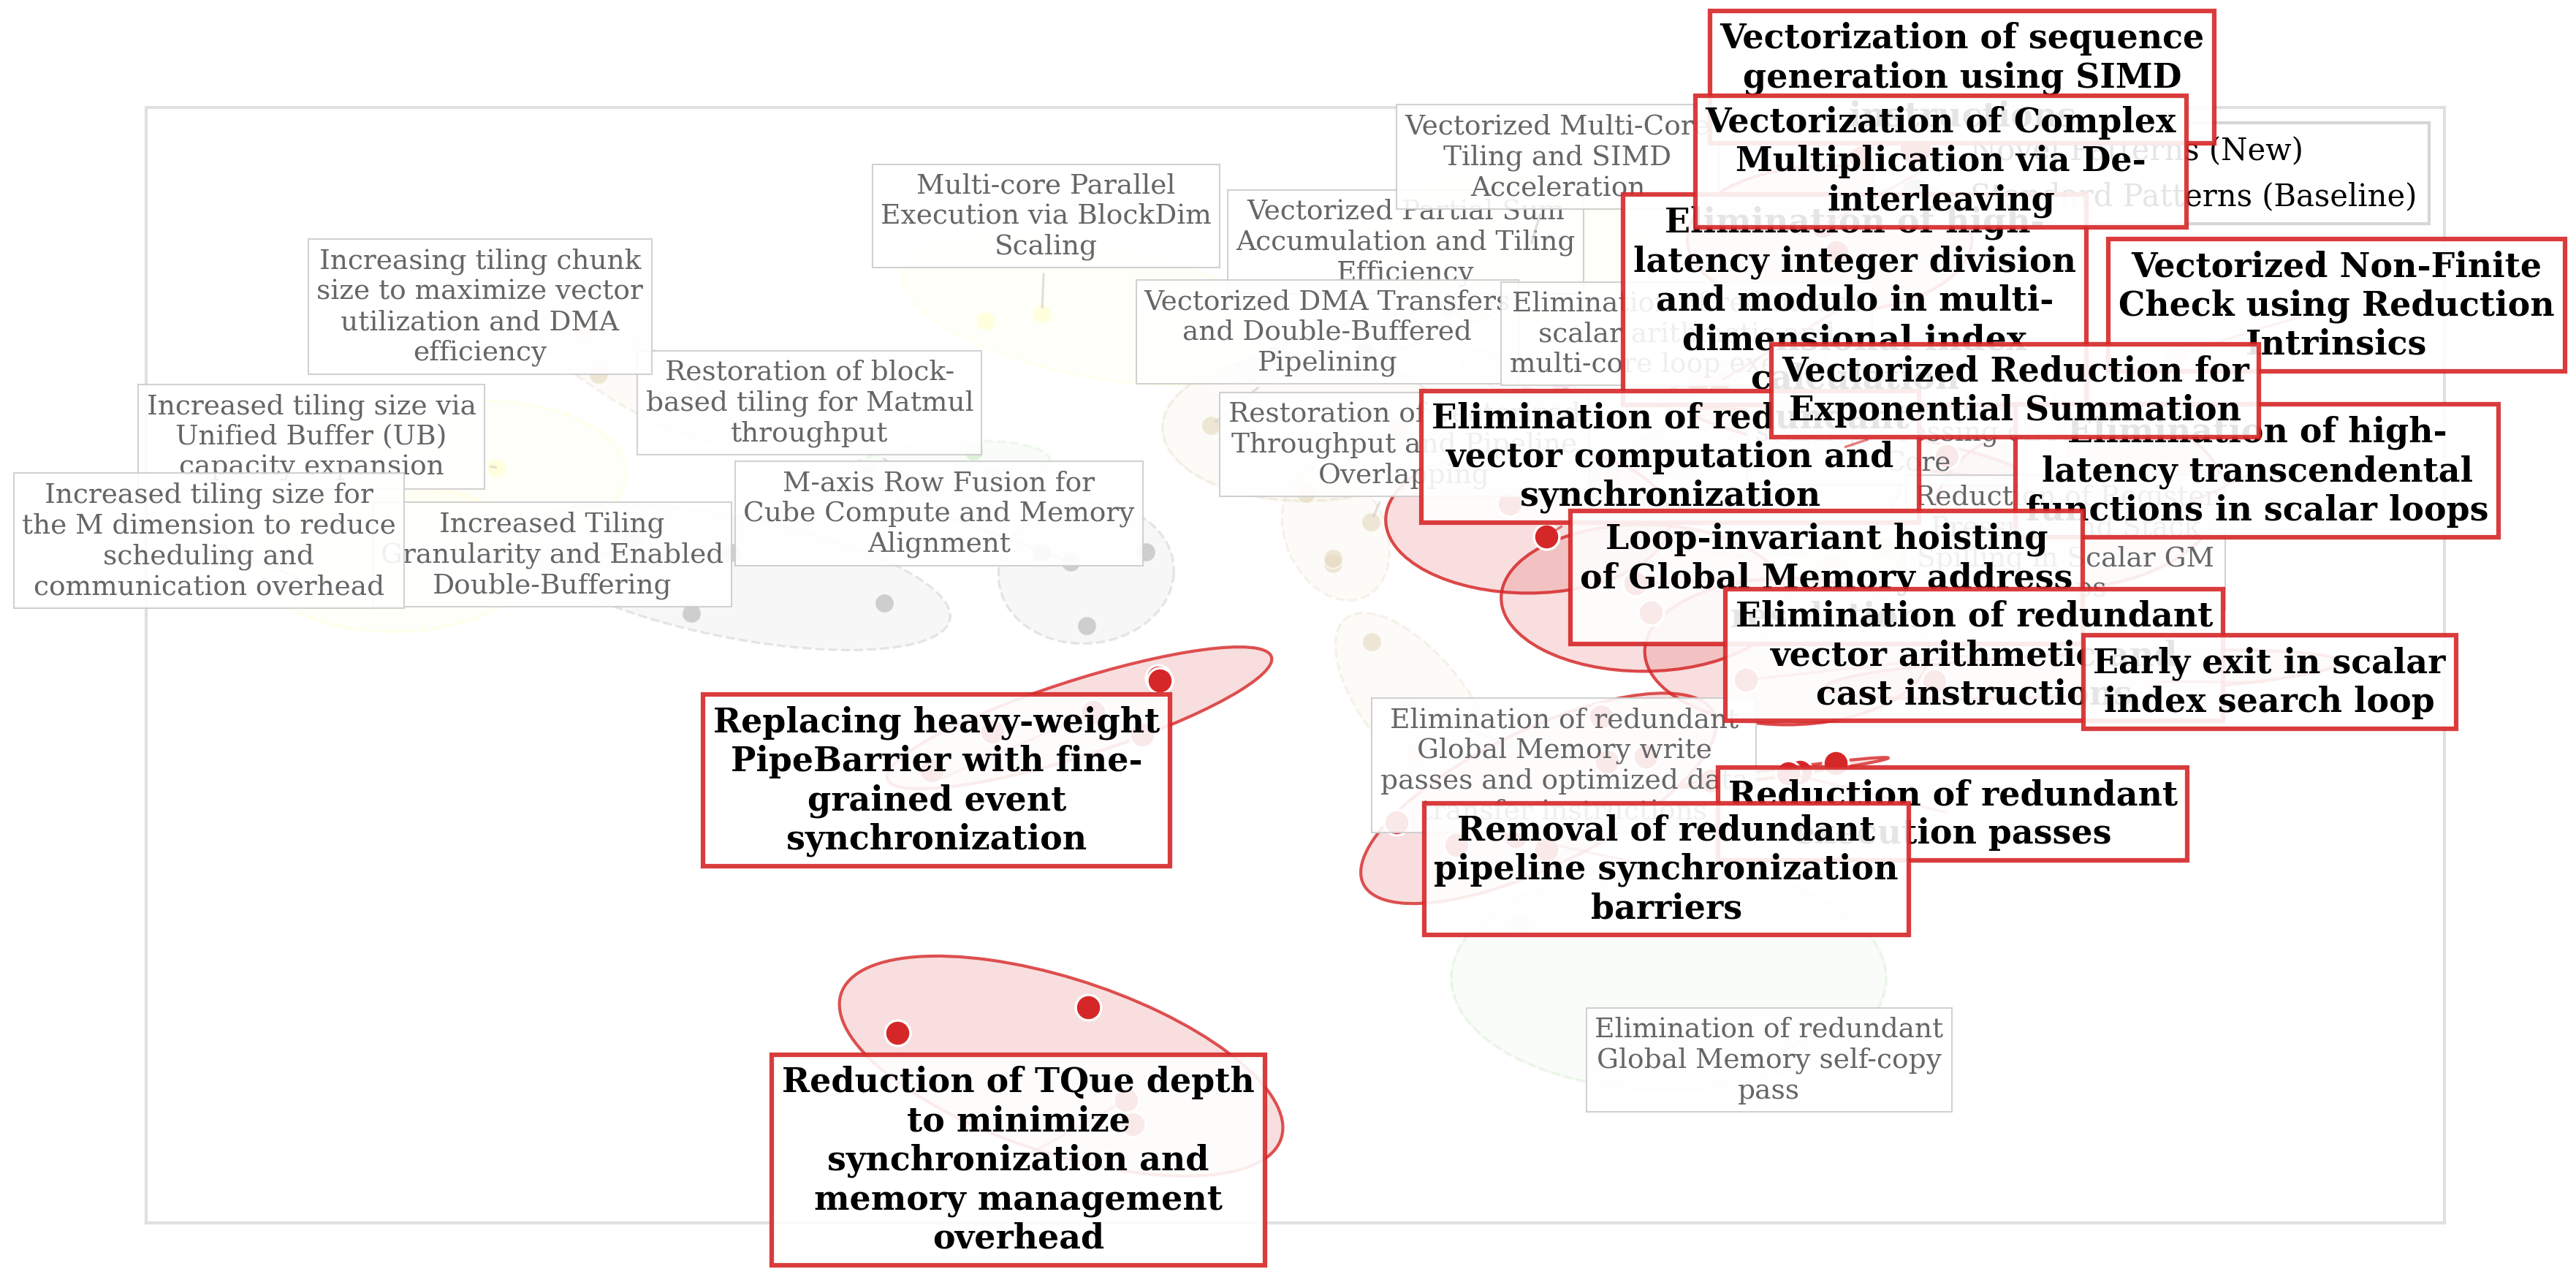
\includegraphics[width=0.65\textwidth]{fig/cluster_scatter_llm.png}
% \caption{Semantic landscape of optimization strategies via embedding clustering.
% Each optimization record (Title \& Description) is embedded using an embedding model, projected to 2D for visualization with PCA, and clustered with K-Means.
% Grey/light regions denote clusters aligned with categories described in the official documentation, while red regions denote clusters that do not directly correspond to the documentation’s explicit taxonomy.}
% \label{fig:semantic_landscape}
% \end{figure*}
% \section{Optimization Trajectory}
% \label{case_2}
% \subsection{Baseline}
% \begin{promptbox}{Baseline}
% ...
%     int64_t tempPerCoreCount = blockCount / needCoreNum * elementsPerBlock;
%     int64_t remainderCount = blockCount % needCoreNum;
%     uint16_t coreIndex = 0;
%     int64_t dataCount = 0;
%     int64_t curCmpCount = 0;
%     int64_t cursorPosition = 0;
%     tensorStartList[coreIndex] = 0;
%     tensorStartOffsetList[coreIndex] = 0;
%     for (uint16_t i = 0; i < totalTensorCount; i++) {
%         curCmpCount = (remainderCount && coreIndex < remainderCount) ? (tempPerCoreCount + elementsPerBlock)
%                                                                      : tempPerCoreCount;
%         int64_t tempCount = tensorDataCountList[i] - cursorPosition;

%         if (dataCount + tempCount < curCmpCount) {
%             dataCount += tempCount;
%             cursorPosition = 0;
%             continue;
%         }

%         tensorEndList[coreIndex] = i;
%         cursorPosition = cursorPosition + curCmpCount - dataCount;
%         tensorEndOffsetList[coreIndex] = cursorPosition - 1;
%         dataCount = 0;
%         coreIndex++;
%         if (cursorPosition < tensorDataCountList[i]) {
%             tensorStartList[coreIndex] = i;
%             tensorStartOffsetList[coreIndex] = cursorPosition;
%             --i;
%         } else if (coreIndex != needCoreNum) {
%             tensorStartList[coreIndex] = i + 1;
%             tensorStartOffsetList[coreIndex] = 0;
%             cursorPosition = 0;
%         }
%     }

%     if (dataCount) {
%         tensorEndList[coreIndex] = totalTensorCount - 1;
% ...
% \end{promptbox}


\subsection{Method Details}\label{app:methodDet}
\begin{tcolorbox}[
  enhanced,
  breakable,
  colback=white,
  colframe=black!30,
  boxrule=0.3pt,
  arc=1.2pt,
  left=0.5em,right=0.5em,top=0.5em,bottom=0.5em,
  title={Method details: base tiling function $\mathcal{T}_{\text{base}}$},
  fonttitle=\bfseries,
]
\lstset{style=appendixcode}
\begin{lstlisting}

// # evolve_tiling_block_start
std::map<std::string, int64_t> AdaptiveTilingStrategy(const std::vector<int64_t>& xShape,
                                                      const std::vector<int64_t>& srcShape,
                                                      int64_t dim,
                                                      const std::string& reduceType,
                                                      bool includeSelf,
                                                      int64_t inputBytes)
{
    constexpr int64_t CORENUM = 1;
    constexpr int64_t BLOCK_BYTES_SIZE = 32;

    std::map<std::string, int64_t> params;
    if (xShape.empty() || srcShape.empty()) {
        return params;
    }

    if (dim < 0 || dim >= static_cast<int64_t>(xShape.size()) ||
        dim >= static_cast<int64_t>(srcShape.size())) {
        return params;
    }

    int64_t batchSize = 1;
    for (int64_t i = 0; i < dim; ++i) {
        batchSize *= xShape[i];
    }

    const int64_t dimSizeX = xShape[dim];
    const int64_t dimSizeSrc = srcShape[dim];

    int64_t strideSize = 1;
    for (int64_t i = dim + 1; i < static_cast<int64_t>(xShape.size()); ++i) {
        strideSize *= xShape[i];
    }

    int64_t reduction = 0;
    if (reduceType == "sum") {
        reduction = 0;
    } else if (reduceType == "prod") {
        reduction = 1;
    } else if (reduceType == "mean") {
        reduction = 2;
    } else if (reduceType == "amax") {
        reduction = 3;
    } else if (reduceType == "amin") {
        reduction = 4;
    }

    int64_t blockSize = (inputBytes > 0) ? (BLOCK_BYTES_SIZE / inputBytes) : BLOCK_BYTES_SIZE;
    if (blockSize <= 0) {
        blockSize = 1;
    }

    const int64_t blockNum = (strideSize + blockSize - 1) / blockSize;
    const int64_t coreNum = std::min<int64_t>(CORENUM, blockNum == 0 ? CORENUM : blockNum);

    const bool specialCase = (batchSize == 1 && dimSizeX == dimSizeSrc && !includeSelf &&
                              reduction == 4 && inputBytes == 4);
    const int64_t blockDim = specialCase ? coreNum : 0;

    params["batchSize"] = batchSize;
    params["dimSizeX"] = dimSizeX;
    params["dimSizeSrc"] = dimSizeSrc;
    params["strideSize"] = strideSize;
    params["reduction"] = reduction;
    params["includeSelf"] = includeSelf ? 1 : 0;
    params["blockSize"] = blockSize;
    params["blockNum"] = blockNum;
    params["blockDim"] = blockDim;
    params["specialCaseFlag"] = specialCase ? 1 : 0;

    return params;
}
// # evolve_tiling_block_end

\end{lstlisting}
\end{tcolorbox}
\captionof{figure}{Base tiling function $\mathcal{T}_{\text{base}}$ with evolution markers, synthesized from the operator code and attributes $\mathcal{S}$.}
\label{fig:appendix_tiling_code}

\begin{tcolorbox}[
  enhanced,
  breakable,
  colback=white,
  colframe=black!30,
  boxrule=0.3pt,
  arc=1.2pt,
  left=0.5em,right=0.5em,top=0.5em,bottom=0.5em,
  title={Method details: optimization thought from rewind},
  fonttitle=\bfseries,
]
\lstset{style=appendixcode}
\begin{lstlisting}
"optimization_point": {
      "title": "Elimination of Pipeline Serialization and Enhancement of DMA Transfer Efficiency",
      "description": "The Fast Version achieves significantly higher performance by addressing three critical architectural inefficiencies present in the Slow Version:

1) Pipeline pipelining:
   - The Slow Version invokes `PipeBarrier<PIPE_ALL>()` inside the inner loop for every complex element.
   - On the Ascend AI Core, this forces a full stall across MTE1/MTE2/MTE3 and the Vector units, preventing overlap between data movement and computation.
   - Removing these barriers restores the intended decoupled pipeline and enables instruction-level parallelism.

2) DMA burst efficiency:
   - The Slow Version sets `maxDataCount = 2` (1 complex float = 8 bytes), far below the typical 32B/64B-efficient burst sizes on MTE.
   - Increasing it to `maxDataCount = 8` (32 bytes) improves the payload-to-overhead ratio for DMA commands.

3) Optimized data paths:
   - Switching from `CopyInPad` (via `DataCopyPad`) to `CopyIn` (via `DataCopy`), and enabling aligned mode in `CopyOut`, allows the operator to take the high-performance aligned DMA path.
   - `DataCopyPad` is generally slower due to extra handling for non-contiguous or unaligned accesses, while `DataCopy` maps more directly to efficient hardware move instructions when alignment is satisfied.",
      "bottleneck": "The primary bottleneck is the intentional serialization of the execution pipeline caused by excessive synchronization barriers and extremely small tiling sizes, which prevents the overlapping of memory transfers and vector computations.",
      "code_diff": "
      --- Changes in op_kernel ---
--- Slow/op_kernel
+++ Fast/op_kernel
@@ -62,8 +62,8 @@
     calNum = kernelParam.calNumPerCore;
 
     startOffset = kernelParam.offset;
-    // Shrink tile size even further so each iteration processes just one complex value.
-    maxDataCount = 2;  // elements (1 complex number)
+    // Shrink tile size aggressively so each iteration only handles a few elements, killing burst efficiency.
+    maxDataCount = 8;  // elements (4 complex numbers)
 
     // ub 192kb
     pipe.InitBuffer(xMatQueue, 2, maxDataCount * sizeof(T));    // 54kb
@@ -123,10 +123,9 @@
 __aicore__ inline void ComplexMatDotAIV<T>::SingleIteration(uint64_t offset, uint64_t dataCount,
                                                             LocalTensor<uint32_t> offsetLocal)
 {
-    // Use padded copies even for aligned lengths to avoid the fast aligned DMA path.
-    CopyInPad(offset, dataCount);
+    CopyIn(offset, dataCount);
     Compute(dataCount, offsetLocal);
-    CopyOut(offset, dataCount, 0);
+    CopyOut(offset, dataCount, 1);
 }
 
 template <typename T>
@@ -181,15 +180,8 @@
         T yr = yMatLocal.GetValue(base);
         T yi = yMatLocal.GetValue(base + 1);
 
-        T outReal = xr * yr - xi * yi;
-        T outImag = xr * yi + xi * yr;
-
-        // Force a pipe-wide barrier on every complex element so the loop cannot be pipelined,
-        // intentionally serializing read/compute/write for each value.
-        PipeBarrier<PIPE_ALL>();
-        outMatLocal.SetValue(base, outReal);
-        outMatLocal.SetValue(base + 1, outImag);
-        PipeBarrier<PIPE_ALL>();
+        outMatLocal.SetValue(base, xr * yr - xi * yi);
+        outMatLocal.SetValue(base + 1, xr * yi + xi * yr);
     }
 
     outMatQueue.EnQue<T>(outMatLocal);
      "
    }
\end{lstlisting}
\end{tcolorbox}
\captionof{figure}{optimization thought example: key changes from a slow to a fast implementation. The figure shows a diff for \texttt{ComplexMatDotAIV}, illustrating how (i) adjusting the tiling granularity, (ii) using the aligned \texttt{DataCopy} path, and (iii) removing per-element \texttt{PipeBarrier} synchronizations improve burst efficiency and restore pipelined execution.}
\label{fig:appendix_optimization_thought}

\section{Use of LLMs}\label{sec:llm}
We use LLMs for polish writing. 
Specifically, LLMs assist in refining the grammar, clarity, and overall presentation of the paper, ensuring that the text is clear and professionally written. 
No experimental results or core content were generated by LLMs.


\end{document}

% This document was modified from the file originally made available by
% Pat Langley and Andrea Danyluk for ICML-2K. This version was created
% by Iain Murray in 2018, and modified by Alexandre Bouchard in
% 2019 and 2021 and by Csaba Szepesvari, Gang Niu and Sivan Sabato in 2022.
% Modified again in 2023 and 2024 by Sivan Sabato and Jonathan Scarlett.
% Previous contributors include Dan Roy, Lise Getoor and Tobias
% Scheffer, which was slightly modified from the 2010 version by
% Thorsten Joachims & Johannes Fuernkranz, slightly modified from the
% 2009 version by Kiri Wagstaff and Sam Roweis's 2008 version, which is
% slightly modified from Prasad Tadepalli's 2007 version which is a
% lightly changed version of the previous year's version by Andrew
% Moore, which was in turn edited from those of Kristian Kersting and
% Codrina Lauth. Alex Smola contributed to the algorithmic style files.
